%==============================================================================
% DOKUMEN UTAMA - SKRIPSI/TUGAS AKHIR
%==============================================================================
\documentclass[12pt, a4paper, oneside]{report}

%------------------------------------------------------------------------------
% PAKET-PAKET
%------------------------------------------------------------------------------
\usepackage[T1]{fontenc}
\usepackage[utf8]{inputenc}
\usepackage[indonesian]{babel}
\usepackage{geometry}
\usepackage{graphicx}
\usepackage{amsmath, amssymb, amsthm}
\usepackage{hyperref}
\usepackage{setspace}
\usepackage{parskip}
\usepackage{fancyhdr}
\usepackage{titlesec}
\usepackage{tocloft}
\usepackage{caption}
\usepackage{subcaption}
\usepackage{booktabs}
\usepackage{longtable}
\usepackage{multirow}
\usepackage{xcolor}
\usepackage{listings}
\usepackage{algorithm}
\usepackage{algpseudocode}
\usepackage{natbib}
\usepackage{lipsum} % placeholder text, hapus saat selesai

%------------------------------------------------------------------------------
% PENGATURAN HALAMAN
%------------------------------------------------------------------------------
\geometry{
  top    = 3cm,
  bottom = 3cm,
  left   = 4cm,
  right  = 3cm
}

\doublespacing % spasi 2

%------------------------------------------------------------------------------
% PENGATURAN HYPERREF
%------------------------------------------------------------------------------
\hypersetup{
  colorlinks = true,
  linkcolor  = black,
  citecolor  = black,
  urlcolor   = blue,
  pdftitle   = {Judul Skripsi},
  pdfauthor  = {Nama Penulis},
}

%------------------------------------------------------------------------------
% PENGATURAN HEADER/FOOTER
%------------------------------------------------------------------------------
\setlength{\headheight}{14.5pt}
\pagestyle{fancy}
\fancyhf{}
\fancyhead[R]{\thepage}
\renewcommand{\headrulewidth}{0pt}

%------------------------------------------------------------------------------
% PENGATURAN LISTINGS (KODE PROGRAM)
%------------------------------------------------------------------------------
\lstset{
  basicstyle    = \ttfamily\small,
  keywordstyle  = \color{blue}\bfseries,
  commentstyle  = \color{gray}\itshape,
  stringstyle   = \color{red},
  numbers       = left,
  numberstyle   = \tiny\color{gray},
  stepnumber    = 1,
  breaklines    = true,
  frame         = single,
  captionpos    = b,
}

%==============================================================================
% DOKUMEN MULAI
%==============================================================================
\begin{document}

%------------------------------------------------------------------------------
% HALAMAN JUDUL
%------------------------------------------------------------------------------
\begin{titlepage}
  \centering
  \vspace*{1cm}

  {\Large\bfseries JUDUL SKRIPSI DITULIS DI SINI\\BISA DUA BARIS JIKA PANJANG\par}

  \vspace{1.5cm}

  {\large SKRIPSI\par}

  \vspace{0.5cm}

  {\normalsize
    Diajukan untuk memenuhi salah satu syarat memperoleh gelar\\
    Sarjana \ldots{} pada Program Studi \ldots{}
  \par}

  \vspace{2cm}

  
\includegraphics[width=4cm]{assets/logo_universitas.png}

  \vspace{2cm}

  {\normalsize Disusun oleh:\par}
  \vspace{0.3cm}
  {\large\bfseries NAMA LENGKAP\par}
  {\normalsize NIM: 000000000\par}

  \vfill

  {\normalsize
    PROGRAM STUDI \ldots{}\\
    FAKULTAS \ldots{}\\
    UNIVERSITAS \ldots{}\\
    \the\year{}
  \par}
\end{titlepage}


%------------------------------------------------------------------------------
% HALAMAN ROMAWI (PRAKATA, ABSTRAK, DAFTAR ISI, DSB.)
%------------------------------------------------------------------------------
\pagenumbering{roman}
\setcounter{page}{2}

\chapter*{LEMBAR PENGESAHAN}
\addcontentsline{toc}{chapter}{LEMBAR PENGESAHAN}

\begin{singlespacing}

\begin{center}
  {\large\bfseries
    Perancangan Arsitektur Multitenant Berbasis \textit{Shared Database} dan \textit{Shared Schema}
    sebagai Solusi Efisiensi Infrastruktur dan \textit{Provisioning Tenant}
    pada Platform Manajemen Aset, Inventori, dan Rental
  \par}

  \vspace{0.3cm}

  {\normalsize\itshape
    Design of a Multitenant Architecture Based on Shared Database and Shared Schema
    as a Solution for Infrastructure Efficiency and Tenant Provisioning
    in an Asset, Inventory, and Rental Management Platform
  \par}
\end{center}

\vspace{0.3cm}

\begin{center}
  {\normalsize 1302220067\par}
  {\large\bfseries Indra Mahesa\par}
\end{center}

\vspace{0.3cm}

\begin{center}
  Tugas akhir ini telah diterima dan disahkan untuk memenuhi sebagai syarat memperoleh
  gelar pada Program Studi Sarjana Rekayasa Perangkat Lunak\\
  Fakultas Informatika\\
  \vspace{0.2cm}
  Universitas Telkom
\end{center}

\vspace{0.3cm}

\begin{center}
  Bandung, 07 April 2026
\end{center}

\vspace{0.2cm}
\begin{center}
  Menyetujui,
\end{center}

\vspace{1.0cm}

\begin{tabular}{>{\centering\arraybackslash}p{7cm} >{\centering\arraybackslash}p{7cm}}
  Pembimbing I, & Pembimbing II, \\[2.0cm]
  \textbf{Dr.~Eng.~Jati H.~Husen, S.T., M.Eng.} & \textbf{Muhammad, S.T.} \\
  NIP: 20920040 & NIK: 3311041509920001 \\
\end{tabular}

\vspace{1.0cm}

\begin{center}
  Ketua Program Studi Sarjana Rekayasa Perangkat\\
  Lunak,\\[2.0cm]
  \textbf{Dr.~Eng.~Jati H.~Husen, S.T., M.Eng.}\\
  NIP: 20920040
\end{center}

\end{singlespacing}

\chapter*{LEMBAR ORISINALITAS}
\addcontentsline{toc}{chapter}{LEMBAR ORISINALITAS}

Dengan ini saya, Indra Mahesa, menyatakan sesungguhnya bahwa Tugas Akhir saya dengan judul
\textbf{Perancangan Arsitektur Multitenant Berbasis \textit{Shared Database} dan \textit{Shared Schema}
sebagai Solusi Efisiensi Infrastruktur dan \textit{Provisioning Tenant} pada Platform Manajemen Aset,
Inventori, dan Rental} beserta dengan seluruh isinya merupakan hasil karya saya sendiri, dengan tidak
melakukan penjiplakan yang tidak sesuai dengan etika keilmuan yang berlaku dengan masyarakat keilmuan,
serta produk dari tugas akhir ini bukan merupakan hasil dari Generative AI. Saya siap menanggung
risiko/sanksi yang diberikan jika di kemudian hari ditemukan pelanggaran terhadap etika keilmuan dalam
Laporan Tugas Akhir, atau jika ada klaim dari pihak lain terhadap keaslian karya.

\vspace{2cm}

\begin{flushright}
  Bandung, 07 April 2026 \\[2cm]
  \textbf{Indra Mahesa} \\
  NIM. 1302220067
\end{flushright}

\chapter*{Abstrak}
\addcontentsline{toc}{chapter}{Abstrak}

\noindent\textbf{JUDUL SKRIPSI DITULIS DI SINI}

\vspace{0.5cm}

\noindent\textbf{Nama Lengkap}\\
NIM. 1302220067

\vspace{1cm}

\lipsum[1] % Ganti dengan abstrak Bahasa Indonesia (150--250 kata)

\vspace{1cm}

\noindent\textbf{Kata kunci:} kata kunci satu, kata kunci dua, kata kunci tiga

\chapter*{Abstract}
\addcontentsline{toc}{chapter}{Abstract}

\noindent\textbf{THESIS TITLE WRITTEN HERE}

\vspace{0.5cm}

\noindent\textbf{Full Name}\\
Student ID. 000000000

\vspace{1cm}

\lipsum[2] % Replace with English abstract (150--250 words)

\vspace{1cm}

\noindent\textbf{Keywords:} keyword one, keyword two, keyword three

\chapter*{Kata Pengantar}
\addcontentsline{toc}{chapter}{Kata Pengantar}

Puji syukur penulis panjatkan kepada Tuhan Yang Maha Esa atas segala rahmat dan
karunia-Nya sehingga penulis dapat menyelesaikan skripsi yang berjudul
\textbf{``Judul Skripsi Ditulis di Sini''} dengan baik.

Skripsi ini disusun sebagai salah satu syarat untuk memperoleh gelar Sarjana \ldots{}
pada Program Studi \ldots{}, Fakultas \ldots{}, Universitas \ldots{}.

Penulis mengucapkan terima kasih kepada:
\begin{enumerate}
  \item Bapak/Ibu \ldots{} selaku Pembimbing I atas bimbingan dan arahannya.
  \item Bapak/Ibu \ldots{} selaku Pembimbing II atas bimbingan dan arahannya.
  \item Kedua orang tua dan keluarga atas dukungan dan doa yang selalu diberikan.
  \item Seluruh teman-teman yang telah memberikan semangat dan bantuan.
\end{enumerate}

Penulis menyadari bahwa skripsi ini masih jauh dari sempurna. Oleh karena itu,
kritik dan saran yang membangun sangat penulis harapkan demi perbaikan di masa mendatang.

\vspace{1cm}

\begin{flushright}
  Kota, \today \\[1cm]
  Penulis
\end{flushright}


\tableofcontents
\listoffigures
\listoftables

%------------------------------------------------------------------------------
% HALAMAN ISI (ARAB)
%------------------------------------------------------------------------------
\pagenumbering{arabic}
\setcounter{page}{1}

\chapter{Pendahuluan}

\section{Latar Belakang}

Pengelolaan aset dan inventori merupakan bagian penting dalam mendukung aktivitas operasional organisasi karena berkaitan dengan proses pencatatan, pemantauan, dan pengendalian sumber daya perusahaan \cite{ref3}. Pengelolaan aset yang baik dapat mendukung aktivitas operasional organisasi, khususnya dalam proses pemeliharaan, perbaikan, dan pengadaan aset \cite{ref4}. Untuk mendukung proses tersebut, organisasi mulai memanfaatkan sistem informasi manajemen aset yang mampu membantu proses pencatatan, pendataan, serta pengelolaan aset secara lebih terstruktur dan terdokumentasi \cite{ref4}.

Perkembangan teknologi informasi juga mendorong pertumbuhan \textit{platform} digital berbasis
\textit{Software as a Service} (SaaS) yang memungkinkan satu aplikasi digunakan oleh banyak
organisasi dalam satu layanan terpusat \cite{ref3}. Model layanan \textit{SaaS} memberikan
kemudahan bagi organisasi dalam menggunakan aplikasi tanpa harus membangun dan mengelola
infrastruktur sistem secara mandiri. Selain itu, kebutuhan terhadap sistem yang \textit{scalable}
dan mampu mendukung banyak organisasi menyebabkan pendekatan \textit{multitenancy} semakin banyak
diterapkan pada pengembangan aplikasi \textit{SaaS} modern \cite{ref4}.

Pendekatan \textit{multitenancy} memungkinkan satu aplikasi digunakan secara bersama oleh banyak
\textit{tenant} dengan tetap mempertahankan isolasi data masing-masing organisasi
\cite{ref3,ref5}. Dalam implementasinya, setiap \textit{tenant} dapat memiliki pengguna, data,
dan proses operasional yang berbeda-beda sehingga sistem membutuhkan arsitektur yang mampu
mengelola banyak \textit{tenant} tanpa mencampurkan data antar organisasi. Kondisi tersebut
menyebabkan aspek pengelolaan \textit{tenant} dan isolasi data menjadi bagian penting dalam
pengembangan aplikasi berbasis \textit{SaaS}.

Penelitian ini dilakukan pada pengembangan modul \textit{Asset Management}, \textit{Inventory},
dan \textit{Rental} berbasis \textit{web} yang terintegrasi dengan \textit{platform} RTPintar.
Modul yang dikembangkan dirancang untuk dapat digunakan oleh banyak organisasi dalam satu sistem
dengan kebutuhan pengelolaan data dan proses operasional yang berbeda pada setiap \textit{tenant}.

Dalam implementasi aplikasi \textit{SaaS}, terdapat beberapa pendekatan arsitektur \textit{tenant}
yang umum digunakan, seperti \textit{separate database}, \textit{separate schema}, maupun
\textit{shared schema} \cite{ref6}. Pendekatan \textit{separate database} menawarkan tingkat
isolasi data yang tinggi karena setiap \textit{tenant} menggunakan basis data yang terpisah.
Namun, pendekatan tersebut menyebabkan setiap \textit{tenant} memerlukan pengelolaan dan
konfigurasi basis data tersendiri sehingga meningkatkan kompleksitas operasional ketika jumlah
\textit{tenant} terus bertambah \cite{ref7}. Selain itu, pendekatan \textit{database-per-tenant}
juga meningkatkan kebutuhan \textit{resource} infrastruktur dan proses \textit{maintenance} karena
setiap \textit{tenant} memiliki lingkungan penyimpanan data yang terpisah \cite{ref7}.

Sebagai solusi terhadap permasalahan tersebut, arsitektur \textit{multitenant} dengan pendekatan
\textit{shared database} dan \textit{shared schema} memungkinkan seluruh \textit{tenant}
menggunakan basis data dan struktur tabel yang sama \cite{ref6}. Dengan pendekatan tersebut,
\textit{tenant} baru dapat ditambahkan tanpa perlu membuat basis data baru untuk setiap
\textit{tenant} sehingga proses \textit{provisioning} dapat dilakukan lebih cepat \cite{ref8}.
Selain itu, penggunaan \textit{shared database} dan \textit{shared schema} lebih sesuai untuk
aplikasi \textit{SaaS} dengan jumlah \textit{tenant} yang dapat terus bertambah karena pengelolaan
\textit{tenant} dan \textit{resource} sistem dapat dilakukan secara lebih terpusat \cite{ref7}.
Oleh karena itu, pendekatan \textit{shared database} dan \textit{shared schema} dipilih pada
penelitian ini untuk mendukung kebutuhan pengelolaan banyak \textit{tenant} dalam satu
\textit{platform}.

Meskipun memiliki kelebihan dalam penggunaan \textit{resource} yang lebih efektif, implementasi
\textit{shared database} dan \textit{shared schema} memiliki tantangan pada aspek isolasi data
antar \textit{tenant} \cite{ref9}. Penggunaan struktur tabel yang sama menyebabkan seluruh data
\textit{tenant} berada dalam basis data yang sama sehingga kesalahan dalam pengelolaan
\textit{tenant context} maupun kontrol akses dapat menyebabkan terjadinya akses lintas
\textit{tenant} yang tidak sesuai \cite{ref6}. Kondisi tersebut berpotensi menimbulkan kebocoran
data dan ketidaksesuaian akses informasi antar \textit{tenant} apabila mekanisme isolasi
\textit{tenant} tidak diterapkan secara konsisten pada lapisan aplikasi maupun basis data
\cite{ref4} \cite{ref9}.

Berdasarkan kondisi tersebut, penelitian ini berfokus pada perancangan arsitektur
\textit{multitenant} berbasis \textit{shared database} dan \textit{shared schema} pada modul
\textit{Asset Management}, \textit{Inventory}, dan \textit{Rental} berbasis \textit{web} yang
terintegrasi dengan \textit{platform} RTPintar. Penelitian mencakup perancangan mekanisme
\textit{tenant identification} berbasis \textit{middleware}, implementasi \textit{tenant scoping}
pada lapisan aplikasi, perancangan model penyimpanan data \textit{multitenant}, serta proses
\textit{provisioning tenant} otomatis untuk mendukung proses \textit{onboarding tenant} baru.

\section{Rumusan Masalah}

Berdasarkan latar belakang yang telah dipaparkan, maka rumusan masalah dalam penelitian ini
adalah sebagai berikut:

\begin{enumerate}
  \item Bagaimana merancang arsitektur \textit{multitenant} berbasis \textit{shared database} dan
    \textit{shared schema} yang mampu meningkatkan efisiensi infrastruktur serta mendukung
    pengelolaan banyak organisasi dalam satu \textit{platform}?
  \item Bagaimana merancang mekanisme isolasi data dan \textit{provisioning} \textit{tenant} otomatis
    pada arsitektur \textit{multitenant} agar proses \textit{onboarding} organisasi baru dapat dilakukan
    secara konsisten, aman, dan tanpa konfigurasi manual tambahan?
\end{enumerate}

\section{Tujuan dan Manfaat}

Penelitian ini bertujuan untuk merancang arsitektur \textit{multitenant} berbasis \textit{shared database}
dan \textit{shared schema} yang mampu mendukung pengelolaan banyak organisasi dalam satu \textit{platform}
secara efisien. Perancangan arsitektur dilakukan untuk mengatasi keterbatasan pendekatan non
\textit{multitenant} yang menyebabkan kompleksitas pengelolaan sistem dan peningkatan kebutuhan
infrastruktur ketika jumlah \textit{tenant} bertambah. Selain itu, penelitian ini juga bertujuan merancang
mekanisme isolasi data antar \textit{tenant} melalui \textit{tenant scoping} pada lapisan aplikasi serta
merancang proses \textit{provisioning} \textit{tenant} otomatis agar \textit{onboarding} organisasi baru
dapat dilakukan secara konsisten, aman, dan tanpa konfigurasi manual tambahan.

Melalui penelitian ini diharapkan rancangan arsitektur yang dihasilkan dapat memberikan manfaat
praktis dalam mendukung pengembangan \textit{platform} \textit{multi organization} berbasis \textit{web}, khususnya
pada sistem manajemen aset, inventori, dan rental. Pendekatan \textit{multitenant} berbasis
\textit{shared database} dan \textit{shared schema} diharapkan mampu meningkatkan efisiensi
penggunaan \textit{resource} infrastruktur, menyederhanakan pengelolaan \textit{tenant}, serta mendukung
proses \textit{onboarding} \textit{tenant} secara lebih cepat dan terstandarisasi. Selain manfaat praktis,
penelitian ini juga diharapkan dapat menjadi referensi akademik dalam pengembangan penelitian
terkait arsitektur \textit{multitenant}, \textit{tenant isolation}, dan \textit{provisioning} \textit{tenant} pada
sistem \textit{Software as a Service} (\textit{SaaS}).

Keterkaitan antara tujuan penelitian, pengujian yang dilakukan, dan kesimpulan yang diharapkan
disajikan pada Tabel \ref{tab:tujuan_pengujian}.

\begin{table}[H]
  \caption{Tabel keterkaitan antara tujuan, pengujian dan kesimpulan.}
  \label{tab:tujuan_pengujian}
  \centering
  \fontsize{10}{12}\selectfont
  \setlength{\arrayrulewidth}{0.5pt}
  \setlength{\tabcolsep}{4pt}
  \begin{tabular}{|>{\centering\arraybackslash}p{0.5cm}|>{\raggedright\arraybackslash}p{4.3cm}|>{\raggedright\arraybackslash}p{3.5cm}|>{\raggedright\arraybackslash}p{4.3cm}|}
    \hline
    \multicolumn{1}{|>{\centering\arraybackslash}m{0.5cm}|}{\cellcolor{black}\color{white}\textbf{No.}} &
    \multicolumn{1}{>{\centering\arraybackslash}m{4.3cm}|}{\cellcolor{black}\color{white}\textbf{Tujuan}} &
    \multicolumn{1}{>{\centering\arraybackslash}m{3.5cm}|}{\cellcolor{black}\color{white}\textbf{Pengujian}} &
    \multicolumn{1}{>{\centering\arraybackslash}m{4.3cm}|}{\cellcolor{black}\color{white}\textbf{Kesimpulan}} \\
    \hline
    1 &
    Merancang arsitektur \textit{multitenant} berbasis \textit{shared database} dan \textit{shared schema} untuk mendukung pengelolaan banyak organisasi dalam satu \textit{platform} secara efisien &
    Evaluasi efisiensi infrastruktur dan struktur arsitektur \textit{multitenant} &
    Sistem mampu menggunakan satu basis data dan satu skema bersama untuk banyak \textit{tenant} tanpa memerlukan \textit{instance} terpisah \\
    \hline
    2 &
    Merancang mekanisme isolasi data antar \textit{tenant} pada arsitektur \textit{multitenant} &
    Pengujian \textit{tenant isolation} dan \textit{tenant scoping} pada lapisan aplikasi &
    Data antar \textit{tenant} tetap terisolasi dan \textit{tenant} tidak dapat mengakses data milik \textit{tenant} lain \\
    \hline
    3 &
    Merancang mekanisme \textit{provisioning} \textit{tenant} otomatis untuk mendukung \textit{onboarding} \textit{tenant} baru secara lebih efisien &
    Pengujian proses \textit{provisioning} \textit{tenant} otomatis &
    \textit{Tenant} baru dapat dibuat beserta konfigurasi awalnya tanpa proses konfigurasi manual tambahan \\
    \hline
    4 &
    Merancang arsitektur yang mendukung konsistensi pengelolaan sistem \textit{multi organization} &
    Evaluasi konsistensi struktur data dan pengelolaan \textit{tenant} &
    Setiap \textit{tenant} memiliki struktur pengelolaan data dan konfigurasi yang konsisten dalam satu \textit{platform} terpusat \\
    \hline
  \end{tabular}
\end{table}

\section{Batasan Masalah}

Penelitian ini difokuskan pada perancangan arsitektur \textit{multitenant} berbasis \textit{shared database}
dan \textit{shared schema} pada \textit{platform} manajemen aset, inventori, dan rental berbasis \textit{web}. Agar
penelitian lebih terarah dan sesuai dengan ruang lingkup tugas akhir, maka ditetapkan beberapa
batasan masalah sebagai berikut:

\begin{enumerate}
  \item Penelitian difokuskan pada perancangan arsitektur sistem \textit{multitenant} dan tidak membahas
    implementasi penuh seluruh fitur aplikasi pada \textit{platform} manajemen aset, inventori, dan rental.
  \item Model \textit{multitenancy} yang digunakan dibatasi pada pendekatan \textit{shared
    database} dan \textit{shared schema} tanpa membandingkan implementasi secara mendalam dengan
    model \textit{separate database} atau \textit{separated schema}.
  \item Mekanisme isolasi data \textit{tenant} difokuskan pada penerapan \textit{tenant scoping} pada
    lapisan aplikasi dan penggunaan \textit{tenant identifier} pada basis data.
  \item Penelitian tidak membahas mekanisme keamanan lanjutan seperti enkripsi tingkat lanjut,
    \textit{distributed security architecture}, maupun audit keamanan infrastruktur secara
    menyeluruh.
  \item Proses \textit{provisioning} \textit{tenant} dibatasi pada pembuatan \textit{tenant} baru, inisialisasi
    konfigurasi awal \textit{tenant}, serta pengelolaan data dasar yang diperlukan dalam sistem.
  \item Evaluasi penelitian difokuskan pada aspek efisiensi infrastruktur, konsistensi isolasi
    data antar \textit{tenant}, dan efektivitas \textit{provisioning} \textit{tenant} otomatis.
  \item Penelitian difokuskan pada konteks \textit{platform} \textit{multi organization} berbasis \textit{web} dan
    tidak membahas implementasi pada arsitektur \textit{distributed system} atau
    \textit{multi region infrastructure}.
  \item Rancangan arsitektur yang dihasilkan ditujukan sebagai dasar implementasi pada proyek
    \textit{capstone} dan tidak membahas \textit{deployment} sistem pada lingkungan produksi
    berskala besar secara penuh.
\end{enumerate}

\section{Metode Penelitian}

Pendekatan yang digunakan dalam penelitian ini mencakup studi literatur, perancangan sistem,
implementasi, serta pengujian sistem. Pendekatan tersebut digunakan untuk mendukung proses
perancangan arsitektur \textit{multitenant} berbasis \textit{shared database} dan \textit{shared schema}
pada modul \textit{Asset Management}, \textit{Inventory}, dan \textit{Rental} berbasis \textit{web}.

Tahapan penelitian dilakukan melalui proses analisis kebutuhan sistem, perancangan arsitektur
\textit{multitenant}, implementasi mekanisme \textit{tenant isolation} dan \textit{provisioning} \textit{tenant},
serta pengujian sistem untuk memastikan pengelolaan data antar \textit{tenant} berjalan sesuai dengan
rancangan yang telah dibuat.

\section{Jadwal Pelaksanaan}

Jadwal pelaksanaan penelitian disusun berdasarkan tahapan perancangan arsitektur \textit{multitenant} yang
meliputi studi literatur, analisis kebutuhan sistem dan identifikasi permasalahan arsitektural
pada pendekatan non \textit{multitenant}, perancangan arsitektur \textit{multitenant} berbasis \textit{shared
database} dan \textit{shared schema}, perancangan mekanisme isolasi data dan \textit{provisioning}
\textit{tenant} otomatis, implementasi prototipe arsitektur sebagai pembuktian konsep, evaluasi kesesuaian
arsitektur terhadap parameter yang telah ditetapkan, serta penyusunan laporan akhir penelitian.
Rincian waktu dan tahapan pelaksanaan penelitian disajikan pada Tabel \ref{tab:jadwal}.

\begin{table}[H]
  \caption{Jadwal Pelaksanaan Tugas Akhir.}
  \label{tab:jadwal}
  \centering
  \fontsize{10}{12}\selectfont
  \setlength{\arrayrulewidth}{0.5pt}
  \setlength{\tabcolsep}{4pt}
  \begin{tabular}{|>{\centering\arraybackslash}p{0.4cm}|>{\raggedright\arraybackslash}p{4.8cm}|>{\centering\arraybackslash}p{1.0cm}|>{\centering\arraybackslash}p{1.0cm}|>{\centering\arraybackslash}p{1.0cm}|>{\centering\arraybackslash}p{1.0cm}|>{\centering\arraybackslash}p{1.0cm}|>{\centering\arraybackslash}p{1.0cm}|}
    \hline
    \multicolumn{1}{|>{\centering\arraybackslash}m{0.4cm}|}{\cellcolor{black}\color{white}\textbf{No.}} &
    \multicolumn{1}{>{\centering\arraybackslash}m{4.8cm}|}{\cellcolor{black}\color{white}\textbf{Deskripsi Tahapan}} &
    \multicolumn{1}{>{\centering\arraybackslash}m{1.0cm}|}{\cellcolor{black}\color{white}\textbf{\shortstack{Bulan\\1}}} &
    \multicolumn{1}{>{\centering\arraybackslash}m{1.0cm}|}{\cellcolor{black}\color{white}\textbf{\shortstack{Bulan\\2}}} &
    \multicolumn{1}{>{\centering\arraybackslash}m{1.0cm}|}{\cellcolor{black}\color{white}\textbf{\shortstack{Bulan\\3}}} &
    \multicolumn{1}{>{\centering\arraybackslash}m{1.0cm}|}{\cellcolor{black}\color{white}\textbf{\shortstack{Bulan\\4}}} &
    \multicolumn{1}{>{\centering\arraybackslash}m{1.0cm}|}{\cellcolor{black}\color{white}\textbf{\shortstack{Bulan\\5}}} &
    \multicolumn{1}{>{\centering\arraybackslash}m{1.0cm}|}{\cellcolor{black}\color{white}\textbf{\shortstack{Bulan\\6}}} \\
    \hline
    1 & Studi Literatur dan Pengumpulan Referensi & \cellcolor{black} & & & & & \tabularnewline
    \hline
    2 & Analisis Kebutuhan Sistem dan Identifikasi Permasalahan & \cellcolor{black} & \cellcolor{black} & & & & \tabularnewline
    \hline
    3 & Perancangan Arsitektur Multitenant & & \cellcolor{black} & \cellcolor{black} & & & \tabularnewline
    \hline
    4 & Perancangan Mekanisme \textit{Tenant Isolation} dan \textit{Provisioning Tenant} & & & \cellcolor{black} & \cellcolor{black} & & \tabularnewline
    \hline
    5 & Implementasi Arsitektur dan Fitur \textit{Multitenancy} & & & & \cellcolor{black} & \cellcolor{black} & \tabularnewline
    \hline
    6 & Evaluasi dan Pengujian Sistem & & & & & \cellcolor{black} & \tabularnewline
    \hline
    7 & Analisis Hasil Pengujian & & & & & \cellcolor{black} & \cellcolor{black} \tabularnewline
    \hline
    8 & Penyusunan dan Revisi Laporan Tugas Akhir & & & & & & \cellcolor{black} \tabularnewline
    \hline
    9 & Persiapan Presentasi dan Sidang Tugas Akhir & & & & & & \cellcolor{black} \tabularnewline
    \hline
  \end{tabular}
\end{table}

\chapter{Tinjauan Pustaka}

\section{Penelitian Terkait}

Penelitian mengenai arsitektur multitenant pada platform berbasis web dan \textit{Software as a
Service} telah banyak dilakukan seiring meningkatnya kebutuhan sistem yang melayani banyak
organisasi dalam satu aplikasi terpusat. Fokus penelitian terdahulu umumnya mencakup perbandingan
model \textit{multitenancy}, mekanisme isolasi data, serta implikasi pemilihan arsitektur terhadap
skalabilitas dan efisiensi infrastruktur. Bagian ini merangkum beberapa penelitian relevan yang
menjadi landasan dalam perancangan arsitektur multitenant pada sistem manajemen aset, inventori,
dan rental.

Mangwani et al. (2023) \cite{ref5} melakukan evaluasi terhadap penerapan arsitektur multitenant
pada aplikasi SaaS dengan membandingkan pendekatan monolitik dan \textit{microservices}. Penelitian
tersebut menunjukkan bahwa arsitektur multitenant mampu meningkatkan efisiensi penggunaan sumber
daya dibandingkan pendekatan \textit{single tenant}, terutama ketika jumlah tenant meningkat.
Namun, studi ini lebih menekankan aspek \textit{deployment} dan performa layanan secara umum,
tanpa membahas secara spesifik implikasi pemilihan model penyimpanan data seperti \textit{shared
schema} terhadap isolasi data dan pengelolaan tenant.

Penelitian oleh Mangwani dan Tokekar (2022) \cite{ref9} menganalisis perilaku sistem SaaS dengan
pendekatan \textit{tenant shared} dan \textit{tenant specific}. Hasil penelitian menunjukkan bahwa
model \textit{tenant shared} lebih efisien dari sisi infrastruktur, tetapi memiliki risiko yang
lebih tinggi terhadap kebocoran data apabila mekanisme isolasi tidak dirancang dengan baik. Studi
ini menegaskan pentingnya pengelolaan konteks tenant dan pengendalian akses pada lapisan aplikasi,
namun tidak membahas bagaimana mekanisme tersebut dirancang secara terintegrasi dalam konteks
sistem manajemen aset dan inventori.

Levchenko dan Taratukhin (2021) \cite{ref7} mengusulkan metode adaptasi arsitektur multitenant
berbasis proses bisnis untuk mendukung fleksibilitas penggunaan sistem oleh berbagai organisasi.
Penelitian ini menyoroti pentingnya desain proses \textit{onboarding} dan pengelolaan tenant yang
terstandarisasi agar sistem dapat digunakan oleh tenant dengan karakteristik operasional yang
berbeda. Meskipun relevan, penelitian ini lebih berfokus pada adaptasi proses bisnis, bukan pada
perancangan arsitektur penyimpanan data berbasis \textit{shared database} dan \textit{shared
schema}.

Sementara itu, Pahl dan Lee (2020) \cite{ref10} membahas pola arsitektur \textit{multitenancy}
pada sistem SaaS dan mengidentifikasi \textit{trade-off} antara model \textit{separate database},
\textit{separated schema}, dan \textit{shared schema}. Penelitian ini memberikan landasan teoritis
mengenai implikasi masing-masing model terhadap isolasi data dan efisiensi infrastruktur. Namun,
kajian tersebut bersifat konseptual dan belum mengaitkan secara langsung penerapan \textit{shared
schema} dengan konteks sistem manajemen aset, inventori, dan rental pada platform multi organisasi.

Berdasarkan penelitian terdahulu tersebut, dapat disimpulkan bahwa sebagian besar studi berfokus
pada evaluasi umum arsitektur multitenant, perbandingan model \textit{deployment}, atau adaptasi
proses bisnis. Masih terbatas penelitian yang secara spesifik membahas perancangan arsitektur
multitenant berbasis \textit{shared database} dan \textit{shared schema} dengan fokus pada
efisiensi infrastruktur serta mekanisme isolasi data dalam sistem manajemen aset, inventori, dan
rental. Oleh karena itu, penelitian ini diarahkan untuk mengisi celah tersebut dengan merancang
arsitektur multitenant yang secara eksplisit mengintegrasikan pemilihan model penyimpanan data,
mekanisme isolasi tenant, dan kebutuhan pengelolaan sistem multi organisasi dalam satu platform
terpusat.

\section{Sistem Informasi Manajemen Aset dan Inventori}

Sistem informasi manajemen aset dan inventori merupakan perangkat lunak yang digunakan untuk
melakukan pencatatan, pemantauan, pengendalian, dan pelaporan aset serta barang milik organisasi
secara terstruktur. Penerapan sistem informasi pada pengelolaan aset terbukti mampu meningkatkan
akurasi data, transparansi operasional, serta efisiensi pemanfaatan sumber daya dibandingkan
pendekatan manual atau pencatatan terpisah \cite{ref1,ref3}. Dalam sistem yang terintegrasi,
informasi mengenai kepemilikan aset, kondisi barang, serta riwayat penggunaan dapat diakses
secara konsisten dan \textit{real time}.

Pada platform yang digunakan oleh banyak organisasi secara bersamaan, sistem manajemen aset dan
inventori menghadapi kompleksitas tambahan dibandingkan sistem satu organisasi. Setiap organisasi
memiliki struktur data, pengguna, dan alur operasional yang berbeda, sehingga pengelolaan data
aset tidak hanya berkaitan dengan fungsi pencatatan, tetapi juga dengan mekanisme pemisahan data
dan pengendalian akses. Tanpa dukungan arsitektur yang tepat, pengelolaan aset pada platform multi
organisasi berpotensi menimbulkan duplikasi data, inkonsistensi informasi, serta kesulitan dalam
pengelolaan sistem secara terpusat.

Oleh karena itu, integrasi sistem manajemen aset, inventori, dan layanan rental pada platform
multi organisasi tidak dapat dipisahkan dari perancangan arsitektur perangkat lunak yang mampu
mendukung pengelolaan data lintas organisasi secara efisien dan terisolasi. Aspek ini menjadikan
sistem manajemen aset dan inventori relevan untuk dikaji tidak hanya dari sisi fungsional, tetapi
juga dari perspektif arsitektur sistem.

\section{Konsep \textit{Cloud Computing} dan SaaS}

\textit{Cloud computing} menyediakan infrastruktur komputasi yang elastis, terdistribusi, dan
dapat diakses secara \textit{on demand}, sehingga memungkinkan pengembangan dan pengelolaan
aplikasi berskala besar dengan efisiensi sumber daya yang lebih baik \cite{ref2}. Dalam konteks
\textit{Software as a Service}, aplikasi disediakan sebagai layanan yang dapat diakses melalui
jaringan tanpa memerlukan instalasi lokal, dengan model penggunaan yang mendukung banyak pengguna
dan organisasi secara bersamaan.

Arsitektur SaaS memungkinkan satu aplikasi digunakan oleh banyak organisasi melalui satu sistem
terpusat, sehingga mengurangi biaya operasional, menyederhanakan proses pemeliharaan, dan
mempermudah pembaruan sistem \cite{ref5}. Namun, implementasi SaaS tidak selalu identik dengan
arsitektur multitenant. Banyak sistem SaaS masih dibangun menggunakan pendekatan non multitenant
atau \textit{single tenant}, di mana setiap organisasi memiliki konfigurasi atau \textit{instance}
sistem tersendiri. Pendekatan tersebut berpotensi menimbulkan keterbatasan skalabilitas dan
efisiensi ketika jumlah organisasi pengguna meningkat.

Dalam konteks platform layanan multi organisasi berskala nasional, pemilihan arsitektur SaaS yang
tepat menjadi krusial. Arsitektur yang tidak dirancang untuk penggunaan bersama oleh banyak tenant
akan meningkatkan kompleksitas pengelolaan sistem dan mengurangi manfaat utama dari model SaaS
itu sendiri.

\section{Arsitektur Multitenant}

Arsitektur multitenant merupakan pendekatan perancangan aplikasi di mana satu \textit{instance}
aplikasi digunakan oleh banyak tenant secara bersamaan, dengan tetap menjaga isolasi data,
konfigurasi, dan proses operasional antar tenant \cite{ref4}. Tenant dalam arsitektur multitenant
didefinisikan sebagai entitas organisasi independen yang memiliki data, pengguna, dan alur kerja
tersendiri dalam satu sistem bersama.

Berbagai penelitian mengidentifikasi beberapa pola utama dalam penerapan \textit{multitenancy},
yaitu \textit{shared schema}, \textit{separated schema}, dan \textit{separate database}, yang
masing-masing memiliki karakteristik dan \textit{trade-off} pada aspek isolasi data, biaya
infrastruktur, dan skalabilitas sistem \cite{ref6}. Model \textit{separate database} menawarkan
isolasi data yang tinggi, namun membutuhkan sumber daya dan biaya pengelolaan yang besar.
Sebaliknya, model \textit{shared schema} menawarkan efisiensi infrastruktur dan kemudahan
pengelolaan, tetapi memerlukan mekanisme isolasi data yang lebih ketat pada lapisan aplikasi.

Model \textit{shared database} dan \textit{shared schema} banyak direkomendasikan untuk platform
SaaS tahap awal dan sistem berskala besar karena mampu mendukung pertumbuhan jumlah tenant dengan
biaya infrastruktur yang relatif rendah serta menyederhanakan proses pemeliharaan sistem
\cite{ref9,ref10}. Pemilihan model ini selaras dengan kebutuhan efisiensi infrastruktur dan
pengelolaan data banyak organisasi dalam satu platform terpusat, sebagaimana menjadi fokus
penelitian ini.

\section{Isolasi Data pada Sistem Multitenant}

Isolasi data merupakan aspek kritis dalam arsitektur multitenant untuk memastikan bahwa setiap
tenant hanya dapat mengakses data yang menjadi miliknya. Isolasi data dapat diterapkan pada
beberapa lapisan sistem, yaitu lapisan basis data, lapisan aplikasi, dan lapisan infrastruktur
\cite{ref5,ref8,ref9}.

Pada lapisan basis data, isolasi dapat dilakukan melalui penggunaan atribut identitas tenant
seperti \texttt{tenant\_id}, pemisahan skema, atau pemisahan basis data. Pada lapisan aplikasi,
isolasi diwujudkan melalui mekanisme \textit{tenant aware middleware}, pengelolaan konteks tenant,
serta pembatasan akses berbasis peran. Sementara itu, pada lapisan infrastruktur, isolasi
dilakukan melalui segmentasi sumber daya dan pengendalian beban kerja per tenant.

Penelitian empiris menunjukkan bahwa pendekatan \textit{tenant shared} lebih efisien secara biaya
dan sumber daya dibandingkan pendekatan \textit{tenant specific}, namun memerlukan desain isolasi
logis yang ketat untuk menjaga keamanan dan konsistensi data \cite{ref9}. Oleh karena itu, dalam
konteks arsitektur multitenant berbasis \textit{shared schema}, fokus isolasi data lebih diarahkan
pada pengelolaan konteks tenant dan \textit{tenant scoping} pada lapisan aplikasi, yang menjadi
salah satu fokus utama penelitian ini.

\section{\textit{Tenant Provisioning}}

\textit{Tenant provisioning} merupakan proses pembuatan dan inisialisasi tenant baru dalam sistem
multitenant, yang meliputi konfigurasi awal, inisialisasi metadata, pembentukan entitas organisasi,
serta penetapan peran pengguna awal \cite{ref7}. Dalam sistem non multitenant, proses ini umumnya
dilakukan secara manual dan terpisah untuk setiap organisasi, sehingga meningkatkan kompleksitas
operasional dan risiko ketidakkonsistenan konfigurasi.

Pada arsitektur multitenant, \textit{provisioning} tenant yang terstandarisasi dan otomatis
menjadi bagian penting dari efisiensi operasional sistem. Otomatisasi \textit{provisioning} tenant
memungkinkan platform untuk menambahkan organisasi baru tanpa memerlukan konfigurasi manual
tambahan, sekaligus memastikan konsistensi struktur data dan kebijakan akses antar tenant. Dengan
demikian, mekanisme \textit{provisioning} tenant tidak hanya bersifat administratif, tetapi juga
berperan sebagai komponen arsitektural yang mendukung skalabilitas dan efisiensi sistem secara
keseluruhan.

\chapter{Perancangan Sistem}

\section{Analisis Kebutuhan Sistem}

Analisis kebutuhan sistem dilakukan untuk mengidentifikasi kebutuhan fungsional dan non fungsional
pada platform manajemen aset, inventori, dan rental berbasis web yang dikembangkan dalam proyek
\textit{capstone}. Tahap analisis kebutuhan dilakukan sebagai dasar dalam perancangan arsitektur
multitenant agar sistem mampu mendukung pengelolaan banyak organisasi dalam satu platform secara
efisien dan terpusat.

Pada platform \textit{multi organization}, setiap organisasi memiliki pengguna, data, serta proses
operasional yang berbeda sehingga sistem memerlukan mekanisme pengelolaan tenant yang mampu
menjaga isolasi data antar organisasi. Selain itu, sistem juga memerlukan mekanisme
\textit{provisioning} tenant yang mendukung proses \textit{onboarding} tenant baru secara lebih
cepat dan konsisten tanpa meningkatkan kompleksitas pengelolaan sistem.

Berdasarkan kebutuhan tersebut, analisis dilakukan terhadap kebutuhan pengelolaan tenant,
kebutuhan isolasi data, kebutuhan \textit{scalability} sistem, serta efisiensi penggunaan
\textit{resource} infrastruktur pada platform \textit{multi organization}. Hasil analisis
kebutuhan ini digunakan sebagai dasar dalam perancangan arsitektur multitenant berbasis
\textit{shared database} dan \textit{shared schema}.

\section{Gambaran Umum Sistem}

Sistem yang dikembangkan merupakan platform manajemen aset, inventori, dan rental berbasis web
yang dirancang untuk mendukung banyak organisasi dalam satu layanan terpusat. Platform ini
memungkinkan setiap organisasi memiliki pengguna, data, dan proses operasional masing-masing
dalam satu aplikasi bersama.

Dalam implementasinya, setiap tenant memiliki kebutuhan pengelolaan data yang terpisah sehingga
sistem memerlukan mekanisme isolasi data untuk memastikan setiap organisasi hanya dapat mengakses
data miliknya sendiri. Selain itu, sistem juga memerlukan mekanisme pengelolaan tenant yang mampu
mendukung \textit{onboarding} tenant baru secara efisien tanpa memerlukan konfigurasi infrastruktur
yang terpisah untuk setiap organisasi.

Untuk mendukung kebutuhan tersebut, sistem dirancang menggunakan pendekatan arsitektur multitenant
berbasis \textit{shared database} dan \textit{shared schema}. Pendekatan ini memungkinkan seluruh
tenant menggunakan aplikasi dan basis data yang sama dengan tetap mempertahankan isolasi data antar
tenant melalui mekanisme \textit{tenant scoping} pada \textit{application layer}.

Pada sistem yang dirancang, pengguna akan melakukan autentikasi ke dalam platform dan setiap proses
akses data akan disesuaikan dengan konteks tenant pengguna yang sedang \textit{login}. Dengan
pendekatan tersebut, platform dapat mendukung pengelolaan banyak tenant secara lebih efisien,
terpusat, dan \textit{scalable} dibandingkan pendekatan non multitenant yang menggunakan
\textit{instance} terpisah untuk setiap organisasi.

Ruang lingkup sistem dalam penelitian ini mencakup pengelolaan data aset, inventori, dan rental
sebagai konteks penerapan arsitektur multitenant. Sistem dirancang untuk mendukung penggunaan oleh
banyak tenant dalam satu platform, dengan mekanisme isolasi data, pengelolaan konteks tenant, dan
\textit{provisioning} tenant otomatis. Penelitian ini tidak mencakup pengembangan antarmuka
pengguna secara detail maupun optimalisasi performa tingkat rendah, melainkan berfokus pada
rancangan arsitektur dan mekanisme pendukung yang memastikan efisiensi infrastruktur dan keamanan
data pada platform multi organisasi.

\begin{figure}[h]
  \centering
  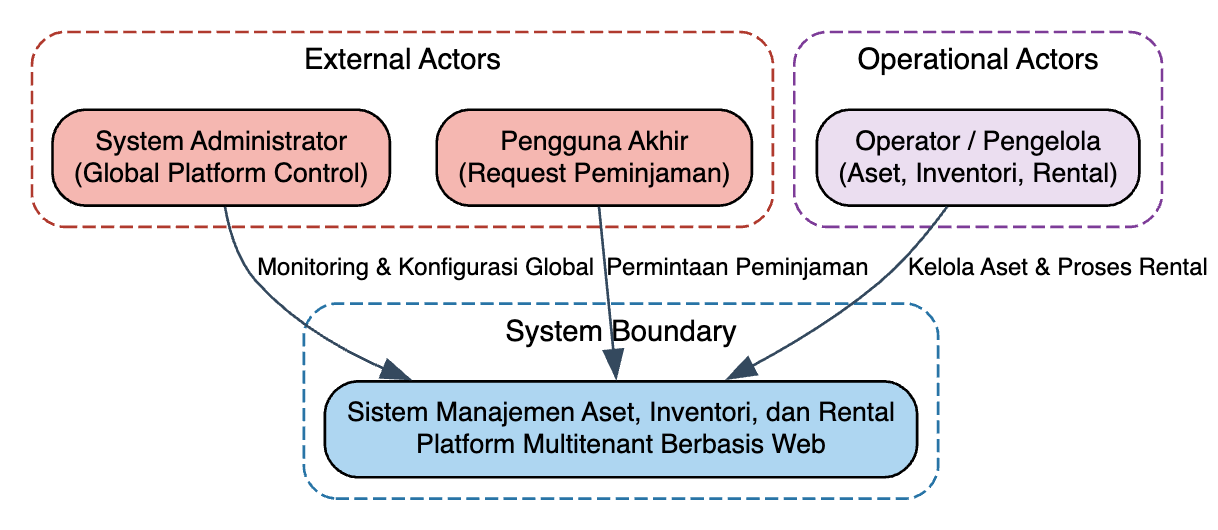
\includegraphics[width=0.9\textwidth]{assets/image2.png}
  \caption{Diagram Konteks Sistem Manajemen Aset, Inventori, dan Rental}
  \label{fig:diagram_konteks}
\end{figure}

\section{Perancangan Arsitektur Multitenant}

Perancangan arsitektur multitenant merupakan inti dari penelitian ini karena berfungsi sebagai
solusi terhadap permasalahan efisiensi infrastruktur dan pengelolaan data multi organisasi dalam
satu platform terpusat. Arsitektur yang dirancang harus mampu melayani banyak tenant secara
bersamaan tanpa mencampurkan data antar tenant, serta tetap efisien dari sisi penggunaan sumber
daya sistem.

\subsection{Pemilihan Arsitektur Multitenant}

Arsitektur yang dipilih dalam penelitian ini adalah arsitektur multitenant berbasis aplikasi
terpusat, di mana satu \textit{instance} aplikasi digunakan oleh seluruh tenant. Setiap permintaan
yang masuk ke sistem diproses dalam konteks tenant tertentu yang ditentukan secara otomatis oleh
sistem pada sisi \textit{server}. Pendekatan ini dipilih untuk menghindari duplikasi aplikasi dan
konfigurasi sistem yang umum terjadi pada pendekatan non multitenant.

Dalam arsitektur ini, tenant diperlakukan sebagai entitas logis, bukan sebagai unit fisik berupa
\textit{instance} aplikasi atau basis data terpisah. Dengan demikian, sistem dapat melayani
pertumbuhan jumlah tenant tanpa perlu menambah \textit{instance} aplikasi baru, sehingga mendukung
skalabilitas dan efisiensi infrastruktur.

\subsection{Justifikasi Pemilihan \textit{Shared Database} dan \textit{Shared Schema}}

Model penyimpanan data yang digunakan adalah \textit{shared database} dan \textit{shared schema},
di mana seluruh tenant menggunakan satu basis data dan satu skema yang sama. Setiap data yang
bersifat spesifik tenant dibedakan menggunakan atribut identitas tenant, seperti
\texttt{tenant\_id}, yang secara konsisten diterapkan pada seluruh operasi basis data.

Pemilihan model ini didasarkan pada beberapa pertimbangan utama. Pertama, \textit{shared schema}
memungkinkan efisiensi penggunaan infrastruktur karena tidak diperlukan basis data atau skema
terpisah untuk setiap tenant. Kedua, pengelolaan sistem menjadi lebih sederhana karena pemeliharaan
dan pembaruan skema dilakukan secara terpusat. Ketiga, model ini mendukung proses
\textit{provisioning} tenant otomatis, karena tenant baru dapat ditambahkan tanpa perlu membuat
struktur basis data baru.

Meskipun model \textit{shared schema} memiliki tantangan terkait isolasi data, risiko tersebut
diatasi melalui mekanisme \textit{tenant scoping} pada lapisan aplikasi, di mana setiap permintaan
dipastikan selalu membawa konteks tenant sebelum diproses lebih lanjut. Dengan pendekatan ini,
isolasi data dijaga secara logis meskipun sumber daya fisik digunakan bersama.

Pada pendekatan non multitenant, setiap organisasi biasanya dikelola melalui \textit{instance}
aplikasi dan basis data terpisah. Pendekatan ini memberikan isolasi data secara fisik, namun
menimbulkan beban infrastruktur yang tinggi, kompleksitas pengelolaan sistem, serta kesulitan
dalam menjaga konsistensi konfigurasi ketika jumlah organisasi meningkat.

Sebaliknya, arsitektur multitenant berbasis \textit{shared database} dan \textit{shared schema}
memungkinkan satu sistem melayani banyak tenant secara bersamaan dengan penggunaan sumber daya
yang lebih efisien. Isolasi data tidak lagi bergantung pada pemisahan fisik, melainkan pada
pengendalian konteks tenant di dalam aplikasi. Perbandingan ini menunjukkan bahwa pendekatan
multitenant lebih sesuai untuk platform layanan multi organisasi berskala nasional yang menuntut
efisiensi dan kemudahan pengelolaan sistem.

\begin{figure}[h]
  \centering
  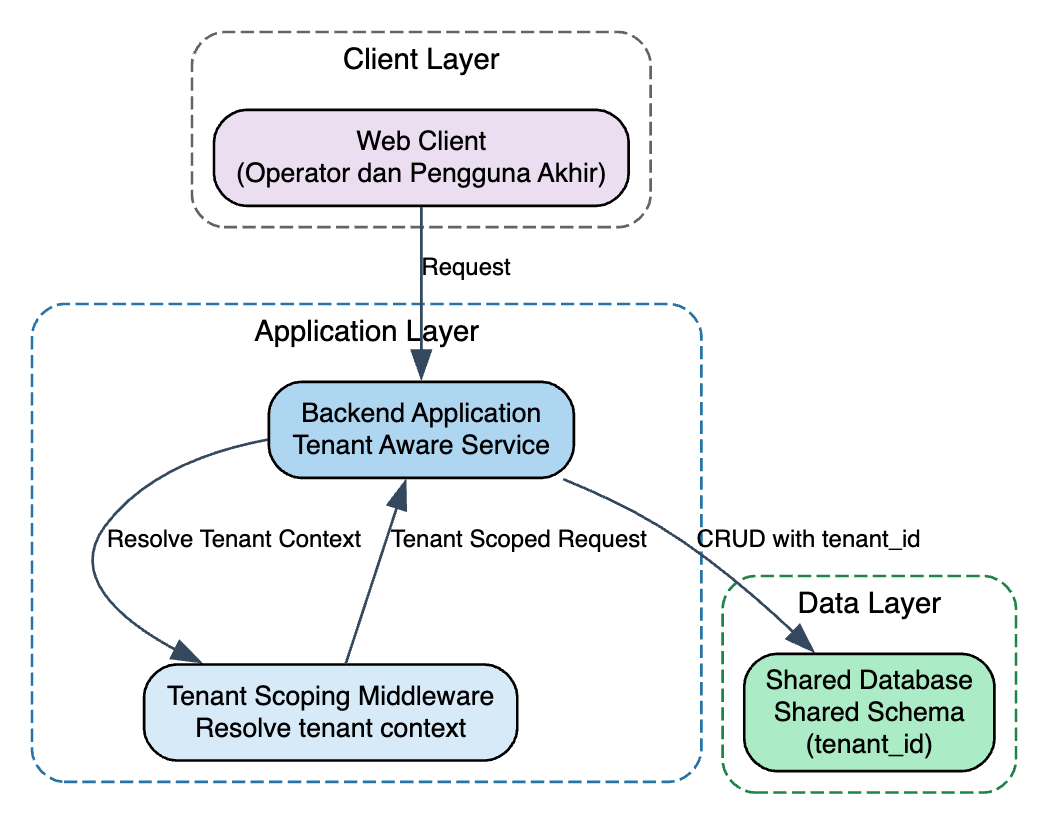
\includegraphics[width=0.9\textwidth]{assets/image3.png}
  \caption{Arsitektur Sistem Multitenant Berbasis \textit{Shared Database} dan \textit{Shared Schema}}
  \label{fig:arsitektur_multitenant}
\end{figure}

\section{Perancangan Model Penyimpanan Data}

Perancangan model penyimpanan data bertujuan untuk menjelaskan bagaimana pendekatan
\textit{shared database} dan \textit{shared schema} diterapkan pada sistem multitenant yang
dirancang. Model ini digunakan untuk mendukung efisiensi infrastruktur dengan tetap menjaga
isolasi data antar tenant melalui mekanisme pemisahan logis pada tingkat skema dan aplikasi.

\subsection{Struktur \textit{Shared Database}}

Sistem menggunakan satu basis data terpusat yang dipakai bersama oleh seluruh tenant. Seluruh
tabel disimpan dalam satu skema basis data yang sama, sehingga tidak terdapat pemisahan fisik
basis data atau skema untuk masing-masing tenant. Pendekatan ini dipilih untuk menyederhanakan
pengelolaan basis data, mengurangi duplikasi struktur data, serta mendukung proses
\textit{provisioning} tenant secara otomatis tanpa memerlukan pembuatan skema baru.

Struktur basis data dibagi menjadi dua kategori utama, yaitu tabel global dan tabel
\textit{tenant scoped}, yang masing-masing memiliki peran berbeda dalam mendukung arsitektur
multitenant.

\subsection{Peran \texttt{tenant\_id} dalam Isolasi Data}

Atribut \texttt{tenant\_id} berfungsi sebagai penanda utama untuk membedakan data milik
masing-masing tenant dalam tabel \textit{tenant scoped}. Setiap \textit{record} yang berkaitan
dengan data operasional organisasi, seperti aset, inventori, dan rental, selalu memiliki nilai
\texttt{tenant\_id} yang mengidentifikasi kepemilikan data tersebut.

Dalam setiap operasi basis data, \texttt{tenant\_id} disertakan secara implisit melalui mekanisme
\textit{tenant scoping} pada lapisan aplikasi. Dengan demikian, seluruh operasi baca dan tulis
data selalu dibatasi pada tenant yang sesuai, sehingga mencegah terjadinya akses data lintas
tenant meskipun seluruh data disimpan dalam satu skema yang sama.

\subsection{Pemisahan Tabel Global dan \textit{Tenant Scoped}}

Tabel global digunakan untuk menyimpan data yang bersifat umum dan tidak terikat pada tenant
tertentu, seperti data konfigurasi sistem global atau metadata yang berlaku untuk seluruh platform.
Tabel global tidak memiliki atribut \texttt{tenant\_id} karena datanya memang dimaksudkan untuk
digunakan bersama oleh seluruh tenant.

Sebaliknya, tabel \textit{tenant scoped} digunakan untuk menyimpan data yang bersifat spesifik
bagi masing-masing tenant. Seluruh tabel \textit{tenant scoped} wajib memiliki atribut
\texttt{tenant\_id} sebagai bagian dari kunci logis data. Pemisahan ini memastikan bahwa hanya
data yang relevan dengan konteks tenant yang dapat diakses dalam setiap operasi sistem.

\begin{figure}[h]
  \centering
  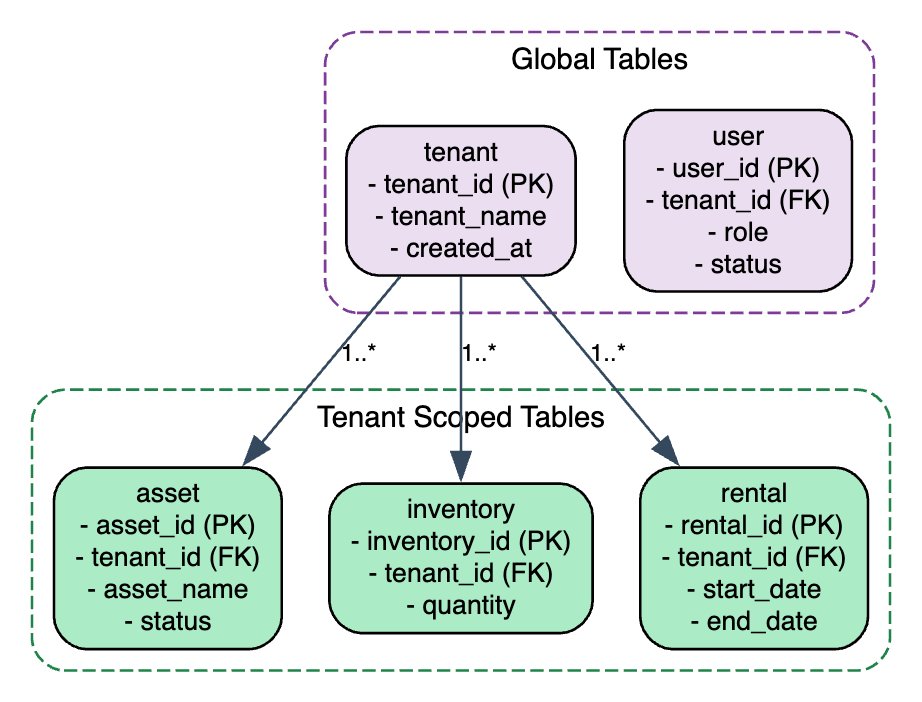
\includegraphics[width=0.9\textwidth]{assets/image4.png}
  \caption{Diagram Konseptual Model Penyimpanan Data \textit{Shared Schema}}
  \label{fig:model_penyimpanan}
\end{figure}

\section{Perancangan Mekanisme Isolasi Data}

Perancangan mekanisme isolasi data bertujuan untuk memastikan bahwa setiap tenant hanya dapat
mengakses data yang berada dalam konteks organisasinya masing-masing, meskipun seluruh tenant
berbagi aplikasi dan basis data yang sama. Pada arsitektur multitenant berbasis \textit{shared
database} dan \textit{shared schema}, isolasi data tidak dicapai melalui pemisahan fisik,
melainkan melalui mekanisme pengendalian konteks tenant pada lapisan aplikasi.

\subsection{\textit{Tenant Scoping} pada Lapisan Aplikasi}

\textit{Tenant scoping} merupakan mekanisme yang digunakan untuk menentukan dan mengelola konteks
tenant pada setiap permintaan yang masuk ke sistem. Dalam sistem yang dirancang, tenant tidak
ditentukan oleh pilihan pengguna secara manual, melainkan diidentifikasi secara otomatis oleh
sistem berdasarkan informasi yang dibawa pada permintaan, seperti token autentikasi atau metadata
permintaan.

Setelah tenant berhasil diidentifikasi, sistem menyimpan informasi \texttt{tenant\_id} ke dalam
konteks permintaan (\textit{request context}). Konteks ini kemudian digunakan secara konsisten
pada seluruh lapisan aplikasi, khususnya pada saat pembentukan \textit{query} basis data. Dengan
pendekatan ini, seluruh operasi data secara implisit dibatasi pada tenant yang sesuai tanpa
memerlukan intervensi pengguna.

\subsection{Alur \textit{Request Tenant Aware}}

Alur \textit{request tenant aware} dirancang agar setiap permintaan yang diproses oleh sistem
selalu berada dalam konteks tenant yang valid. Proses ini dimulai ketika pengguna mengirimkan
permintaan ke \textit{backend} melalui antarmuka web. Permintaan tersebut terlebih dahulu diproses
oleh komponen \textit{middleware tenant scoping} yang bertugas mengekstraksi identitas tenant dari
permintaan dan memverifikasinya.

Apabila identitas tenant valid, \textit{middleware} akan menambahkan \texttt{tenant\_id} ke dalam
konteks permintaan sebelum diteruskan ke lapisan layanan aplikasi. Layanan aplikasi kemudian
mengeksekusi logika bisnis dan operasi basis data dengan menyertakan \texttt{tenant\_id} sebagai
pembatas akses data. Alur \textit{tenant scoping} ini ditunjukkan pada Gambar \ref{fig:alur_tenant_scoping}.

\begin{figure}[h]
  \centering
  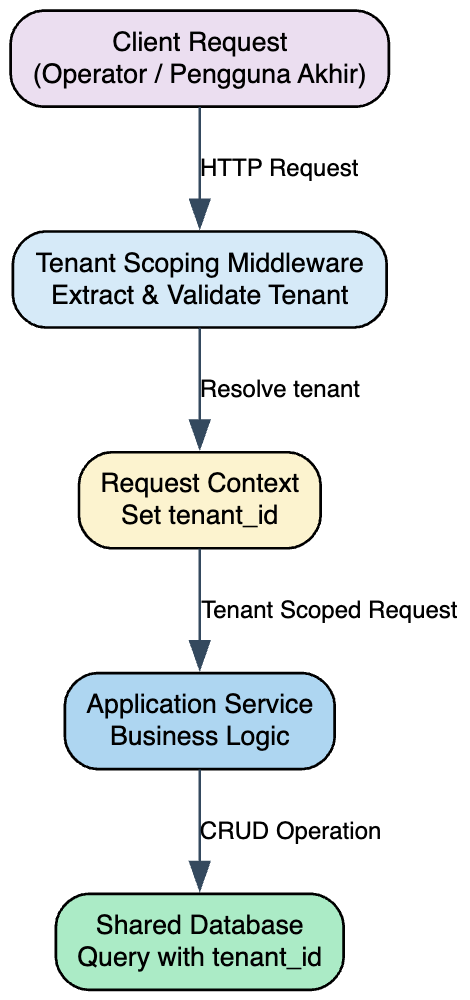
\includegraphics[width=0.45\textwidth]{assets/image5.png}
  \caption{Diagram Alur \textit{Tenant Scoping} pada Lapisan Aplikasi}
  \label{fig:alur_tenant_scoping}
\end{figure}

\subsection{Pembatasan Akses Data}

Pembatasan akses data diterapkan dengan memastikan bahwa setiap \textit{query} basis data terhadap
tabel \textit{tenant scoped} selalu menyertakan kondisi berdasarkan \texttt{tenant\_id}. Pendekatan
ini mencegah kemungkinan akses lintas tenant, baik secara sengaja maupun tidak sengaja. Dengan
menjadikan \texttt{tenant\_id} sebagai bagian wajib dalam seluruh operasi data, sistem dapat
menjamin bahwa data yang diambil atau dimodifikasi selalu sesuai dengan konteks tenant yang aktif.

Selain itu, pembatasan akses juga didukung oleh pengaturan hak akses berbasis peran pada tingkat
aplikasi, sehingga pengguna hanya dapat melakukan operasi yang sesuai dengan perannya dalam
konteks tenant masing-masing. Kombinasi antara \textit{tenant scoping} dan kontrol akses berbasis
peran membentuk mekanisme isolasi data yang konsisten dan terkontrol.

\section{Perancangan Proses \textit{Provisioning} Tenant}

Perancangan proses \textit{provisioning} tenant bertujuan untuk memastikan bahwa penambahan tenant
baru pada sistem multitenant dapat dilakukan secara otomatis, konsisten, dan efisien tanpa
memerlukan konfigurasi manual tambahan. Pada platform multi organisasi berskala nasional, proses
\textit{onboarding} tenant yang tidak terstandarisasi akan meningkatkan kompleksitas operasional
dan berpotensi menimbulkan ketidakkonsistenan konfigurasi sistem.

\subsection{Alur \textit{Provisioning} Tenant Otomatis}

\textit{Provisioning} tenant pada sistem yang dirancang dilakukan sepenuhnya oleh sistem di sisi
\textit{server}. Proses ini dipicu ketika terdapat permintaan pendaftaran organisasi baru atau
inisialisasi tenant melalui mekanisme yang telah ditentukan oleh platform. Sistem kemudian
menjalankan serangkaian langkah terstruktur untuk membentuk tenant baru tanpa keterlibatan aktor
administrator khusus.

Alur \textit{provisioning} dimulai dengan validasi data awal tenant, dilanjutkan dengan pembuatan
identitas tenant pada tabel global, serta inisialisasi konfigurasi standar yang berlaku untuk
seluruh tenant. Setelah proses ini selesai, tenant dinyatakan aktif dan siap digunakan oleh
pengguna operasional. Alur \textit{provisioning} tenant otomatis ini ditunjukkan pada Gambar \ref{fig:provisioning_tenant}.

\begin{figure}[h]
  \centering
  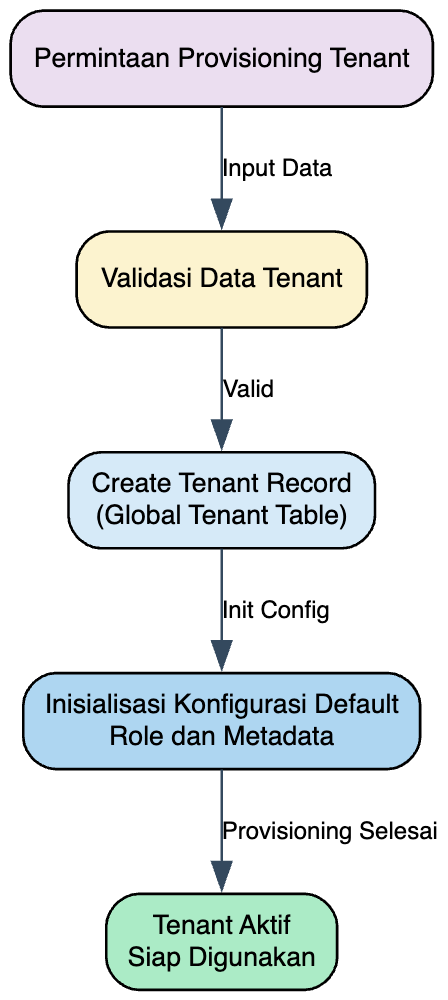
\includegraphics[width=0.45\textwidth]{assets/image6.png}
  \caption{Diagram Proses \textit{Provisioning} Tenant Otomatis}
  \label{fig:provisioning_tenant}
\end{figure}

\subsection{Data dan Konfigurasi yang Diinisialisasi}

Pada saat \textit{provisioning} tenant dilakukan, sistem menginisialisasi sejumlah data dan
konfigurasi dasar agar tenant dapat langsung beroperasi. Data dan konfigurasi tersebut meliputi
identitas tenant, struktur akses dasar, serta metadata yang diperlukan untuk pengelolaan konteks
tenant pada lapisan aplikasi. Seluruh data yang diinisialisasi mengikuti standar yang sama untuk
setiap tenant, sehingga tidak terjadi perbedaan konfigurasi antar tenant yang disebabkan oleh
intervensi manual.

Pendekatan ini memastikan bahwa setiap tenant memiliki struktur data dan konfigurasi awal yang
konsisten, serta dapat langsung menggunakan sistem tanpa memerlukan penyesuaian tambahan pada
tingkat aplikasi maupun basis data.

\subsection{Perbandingan \textit{Provisioning} Manual dan Otomatis}

Pada pendekatan \textit{provisioning} manual, penambahan tenant baru biasanya memerlukan pembuatan
konfigurasi sistem secara terpisah, termasuk penyesuaian basis data, pengaturan akses, dan
validasi konfigurasi. Pendekatan ini tidak efisien dan berisiko menimbulkan kesalahan konfigurasi,
terutama ketika jumlah tenant meningkat.

Sebaliknya, \textit{provisioning} tenant otomatis pada arsitektur multitenant berbasis
\textit{shared database} dan \textit{shared schema} memungkinkan penambahan tenant baru tanpa
perubahan struktur sistem. Seluruh proses dilakukan oleh sistem berdasarkan alur yang telah
ditentukan, sehingga mengurangi beban operasional dan meningkatkan konsistensi konfigurasi.

\section{Rancangan Evaluasi dan Parameter Pengujian}

Rancangan evaluasi disusun untuk memastikan bahwa arsitektur multitenant yang dirancang
benar-benar memenuhi tujuan penelitian serta mampu menjawab permasalahan yang telah dirumuskan.
Evaluasi tidak difokuskan pada pengukuran performa sistem secara kuantitatif tingkat rendah,
melainkan pada kesesuaian rancangan arsitektur terhadap aspek efisiensi infrastruktur, isolasi
data antar tenant, dan efektivitas \textit{provisioning} tenant otomatis.

\subsection{Parameter Evaluasi Efisiensi Infrastruktur}

Efisiensi infrastruktur dievaluasi dengan meninjau sejauh mana arsitektur multitenant berbasis
\textit{shared database} dan \textit{shared schema} mampu mengurangi kebutuhan sumber daya sistem
dibandingkan pendekatan non multitenant. Parameter evaluasi difokuskan pada kompleksitas
konfigurasi sistem dan dependensi infrastruktur yang diperlukan untuk mendukung banyak tenant
dalam satu platform.

Parameter yang digunakan antara lain jumlah konfigurasi sistem yang harus dikelola, jumlah
komponen infrastruktur yang dibutuhkan, serta kebutuhan penyesuaian konfigurasi ketika tenant
baru ditambahkan. Arsitektur dinilai efisien apabila penambahan tenant tidak memerlukan penambahan
\textit{instance} aplikasi atau basis data baru.

\subsection{Parameter Evaluasi Isolasi Data Antar Tenant}

Evaluasi isolasi data bertujuan memastikan bahwa mekanisme \textit{tenant scoping} dan penggunaan
\texttt{tenant\_id} mampu mencegah akses data lintas tenant. Parameter evaluasi difokuskan pada
konsistensi pembatasan data pada setiap operasi basis data dan kemampuan sistem menolak atau
membatasi akses yang berada di luar konteks tenant.

Pengujian dilakukan melalui simulasi permintaan dari tenant yang berbeda untuk memastikan bahwa
data yang dikembalikan oleh sistem selalu sesuai dengan tenant yang aktif. Isolasi data dinyatakan
terpenuhi apabila tidak ditemukan data milik tenant lain pada hasil pengujian.

\subsection{Parameter Evaluasi \textit{Provisioning} Tenant Otomatis}

Evaluasi \textit{provisioning} tenant dilakukan untuk menilai efektivitas proses
\textit{onboarding} tenant tanpa konfigurasi manual tambahan. Parameter evaluasi difokuskan pada
konsistensi konfigurasi tenant baru, keseragaman struktur data awal, serta kemampuan tenant untuk
langsung menggunakan sistem setelah proses \textit{provisioning} selesai.

\textit{Provisioning} tenant dinyatakan berhasil apabila setiap tenant baru memiliki konfigurasi
awal yang identik dan tidak memerlukan penyesuaian tambahan pada tingkat aplikasi maupun basis
data.

\chapter{Hasil Percobaan dan Analisis}

\section{Lingkungan Pengujian}

Pengujian dilakukan untuk memverifikasi implementasi arsitektur \textit{multitenant} yang telah dirancang pada penelitian ini. Fokus pengujian meliputi mekanisme \textit{tenant isolation}, \textit{tenant provisioning}, serta penerapan \textit{shared database} dan \textit{shared schema}. Seluruh pengujian dilakukan pada lingkungan pengembangan (\textit{development environment}) menggunakan aplikasi yang telah diimplementasikan berdasarkan rancangan pada Bab 3.

Pengujian dilakukan melalui antarmuka aplikasi, layanan API, serta verifikasi langsung pada basis data. Penggunaan beberapa metode verifikasi tersebut bertujuan untuk memastikan bahwa hasil pengujian tidak hanya terlihat pada tampilan aplikasi, tetapi juga sesuai dengan data yang tersimpan pada basis data.

\begin{table}[H]
  \centering
  \caption{Lingkungan Pengujian}
  \label{tab:lingkungan_pengujian}
  \begin{tabular}{|p{5cm}|p{8cm}|}
    \hline
    \rowcolor[HTML]{EFEFEF}
    \textbf{Komponen} & \textbf{Spesifikasi} \\
    \hline
    Sistem Operasi & Ubuntu24.04.2 LTS (Noble Numbat) \\
    \hline
    Bahasa Pemrograman & Go 1.24.3 darwin/arm64 \\
    \hline
    Framework HTTP & Gin \\
    \hline
    Basis Data & PostgreSQL 16 \\
    \hline
    API Testing Tool & Postman \\
    \hline
    Database Client & TablePlus \& Mathesar \\
    \hline
    Web Browser & Microsoft Edge \\
    \hline
    Arsitektur Basis Data & \textit{Shared Database} dan \textit{Shared Schema} \\
    \hline
  \end{tabular}
\end{table}

Berdasarkan lingkungan pengujian pada Tabel \ref{tab:lingkungan_pengujian}, seluruh skenario pengujian dilakukan menggunakan konfigurasi yang sama untuk menjaga konsistensi hasil pengujian. Lingkungan tersebut digunakan untuk menjalankan seluruh fitur pada platform manajemen aset, inventori, dan \textit{rental}.

Skenario pengujian yang digunakan pada penelitian ini dijelaskan pada subbab berikutnya.

\section{Skenario Percobaan}

Pengujian dilakukan berdasarkan rancangan pengujian yang telah dijelaskan pada Bab 3. Fokus pengujian meliputi mekanisme \textit{tenant isolation}, \textit{tenant provisioning}, serta implementasi \textit{shared database} dan \textit{shared schema}. Setiap pengujian dilakukan untuk memverifikasi bahwa arsitektur \textit{multitenant} yang diusulkan telah berjalan sesuai dengan kebutuhan sistem dan indikator keberhasilan yang telah ditetapkan.

\subsection{Skenario Pengujian Tenant Isolation}

Pengujian \textit{tenant isolation} dilakukan untuk memastikan bahwa setiap \textit{tenant} hanya dapat mengakses data yang berada dalam ruang lingkup \textit{tenant} yang sesuai. Pengujian menggunakan dua \textit{tenant} yang berbeda, yaitu Tenant A dan Tenant B, yang masing-masing memiliki data operasional tersendiri.

\begin{table}[H]
  \centering
  \caption{Skenario Pengujian \textit{Tenant Isolation}}
  \label{tab:skenario_pengujian_tenant_isolation}
  \footnotesize
  \begin{tabular}{|c|p{6cm}|p{6.5cm}|}
    \hline
    \rowcolor[HTML]{EFEFEF}
    \textbf{No} & \textbf{Langkah Pengujian} & \textbf{Hasil yang Diharapkan} \\
    \hline
    1 & Login sebagai pengguna Tenant A & Pengguna berhasil masuk ke sistem \\
    \hline
    2 & Mengakses data aset Tenant A & Data aset Tenant A berhasil ditampilkan \\
    \hline
    3 & Login sebagai pengguna Tenant B & Pengguna berhasil masuk ke sistem \\
    \hline
    4 & Mengakses data aset Tenant B & Data aset Tenant B berhasil ditampilkan \\
    \hline
    5 & Mencoba mengakses data \textit{tenant} lain & Akses ditolak atau data tidak ditampilkan \\
    \hline
  \end{tabular}
\end{table}

Pengujian dilakukan melalui antarmuka aplikasi, respons API, dan verifikasi data pada basis data untuk memastikan mekanisme isolasi data berjalan dengan baik.

\subsection{Skenario Pengujian Tenant Provisioning}

Pengujian \textit{tenant provisioning} dilakukan untuk memverifikasi proses pembuatan \textit{tenant} baru beserta konfigurasi awal yang dibutuhkan agar \textit{tenant} dapat langsung menggunakan sistem.

\begin{table}[H]
  \centering
  \caption{Skenario Pengujian \textit{Tenant Provisioning}}
  \label{tab:skenario_pengujian_tenant_provisioning}
  \footnotesize
  \begin{tabular}{|c|p{6cm}|p{6.5cm}|}
    \hline
    \rowcolor[HTML]{EFEFEF}
    \textbf{No} & \textbf{Langkah Pengujian} & \textbf{Hasil yang Diharapkan} \\
    \hline
    1 & Mengisi formulir registrasi \textit{tenant} & Data registrasi diterima sistem \\
    \hline
    2 & Mengirim permintaan registrasi & Data \textit{tenant} berhasil dibuat \\
    \hline
    3 & Memeriksa data \textit{role} & \textit{Role} administrator berhasil dibuat \\
    \hline
    4 & Memeriksa data \textit{permission} & \textit{Permission} berhasil dikaitkan dengan \textit{role} administrator \\
    \hline
    5 & Memeriksa data pengguna & Akun administrator berhasil dibuat \\
    \hline
    6 & Login menggunakan akun administrator & Pengguna berhasil masuk ke sistem \\
    \hline
  \end{tabular}
\end{table}

Pengujian ini bertujuan untuk memastikan seluruh proses \textit{onboarding} \textit{tenant} berjalan secara otomatis tanpa memerlukan konfigurasi manual tambahan.

\subsection{Skenario Pengujian Shared Database dan Shared Schema}

Pengujian \textit{shared database} dan \textit{shared schema} dilakukan untuk memastikan bahwa beberapa \textit{tenant} dapat menggunakan basis data dan struktur tabel yang sama tanpa menyebabkan pencampuran data antar \textit{tenant}.

\begin{table}[H]
  \centering
  \caption{Skenario Pengujian \textit{Shared Database} dan \textit{Shared Schema}}
  \label{tab:skenario_pengujian_shared_database}
  \footnotesize
  \begin{tabular}{|c|p{6cm}|p{6.5cm}|}
    \hline
    \rowcolor[HTML]{EFEFEF}
    \textbf{No} & \textbf{Langkah Pengujian} & \textbf{Hasil yang Diharapkan} \\
    \hline
    1 & Tenant A menambahkan data aset & Data berhasil tersimpan \\
    \hline
    2 & Tenant B menambahkan data aset & Data berhasil tersimpan \\
    \hline
    3 & Memeriksa tabel aset pada basis data & Data kedua \textit{tenant} berada pada tabel yang sama \\
    \hline
    4 & Memeriksa atribut \textit{tenant\_id} & Setiap data memiliki identitas \textit{tenant} yang sesuai \\
    \hline
    5 & Mengakses data melalui aplikasi & Data tetap ditampilkan sesuai \textit{tenant} yang aktif \\
    \hline
  \end{tabular}
\end{table}

Melalui skenario tersebut, dapat diverifikasi bahwa pendekatan \textit{shared database} dan \textit{shared schema} mampu mendukung penggunaan oleh banyak \textit{tenant} tanpa mengurangi kemampuan sistem dalam memisahkan data antar \textit{tenant}.

\section{Hasil Pengujian}

\subsection{Hasil Pengujian Tenant Isolation}

Pengujian \textit{tenant isolation} dilakukan untuk memverifikasi bahwa setiap \textit{tenant} hanya dapat mengakses data yang berada dalam ruang lingkup \textit{tenant} yang sesuai. Pengujian ini merupakan salah satu aspek penting dalam penelitian karena arsitektur yang diusulkan menggunakan pendekatan \textit{shared database} dan \textit{shared schema}. Pada pendekatan tersebut, seluruh \textit{tenant} menggunakan basis data dan struktur tabel yang sama sehingga diperlukan mekanisme yang mampu menjaga pemisahan data antar \textit{tenant}.

Pengujian dilakukan menggunakan dua \textit{tenant} yang berbeda, yaitu Tenant A dengan akun administrator \textbf{gab@test.com} dan Tenant B dengan akun administrator \textbf{indramahesa128@gmail.com}. Kedua \textit{tenant} memiliki data aset yang tersimpan pada tabel yang sama, namun dibedakan menggunakan atribut \textit{tenant\_id}. Pengujian dilakukan melalui antarmuka aplikasi, layanan API, dan pemeriksaan langsung pada basis data.

\begin{figure}[H]
  \centering
  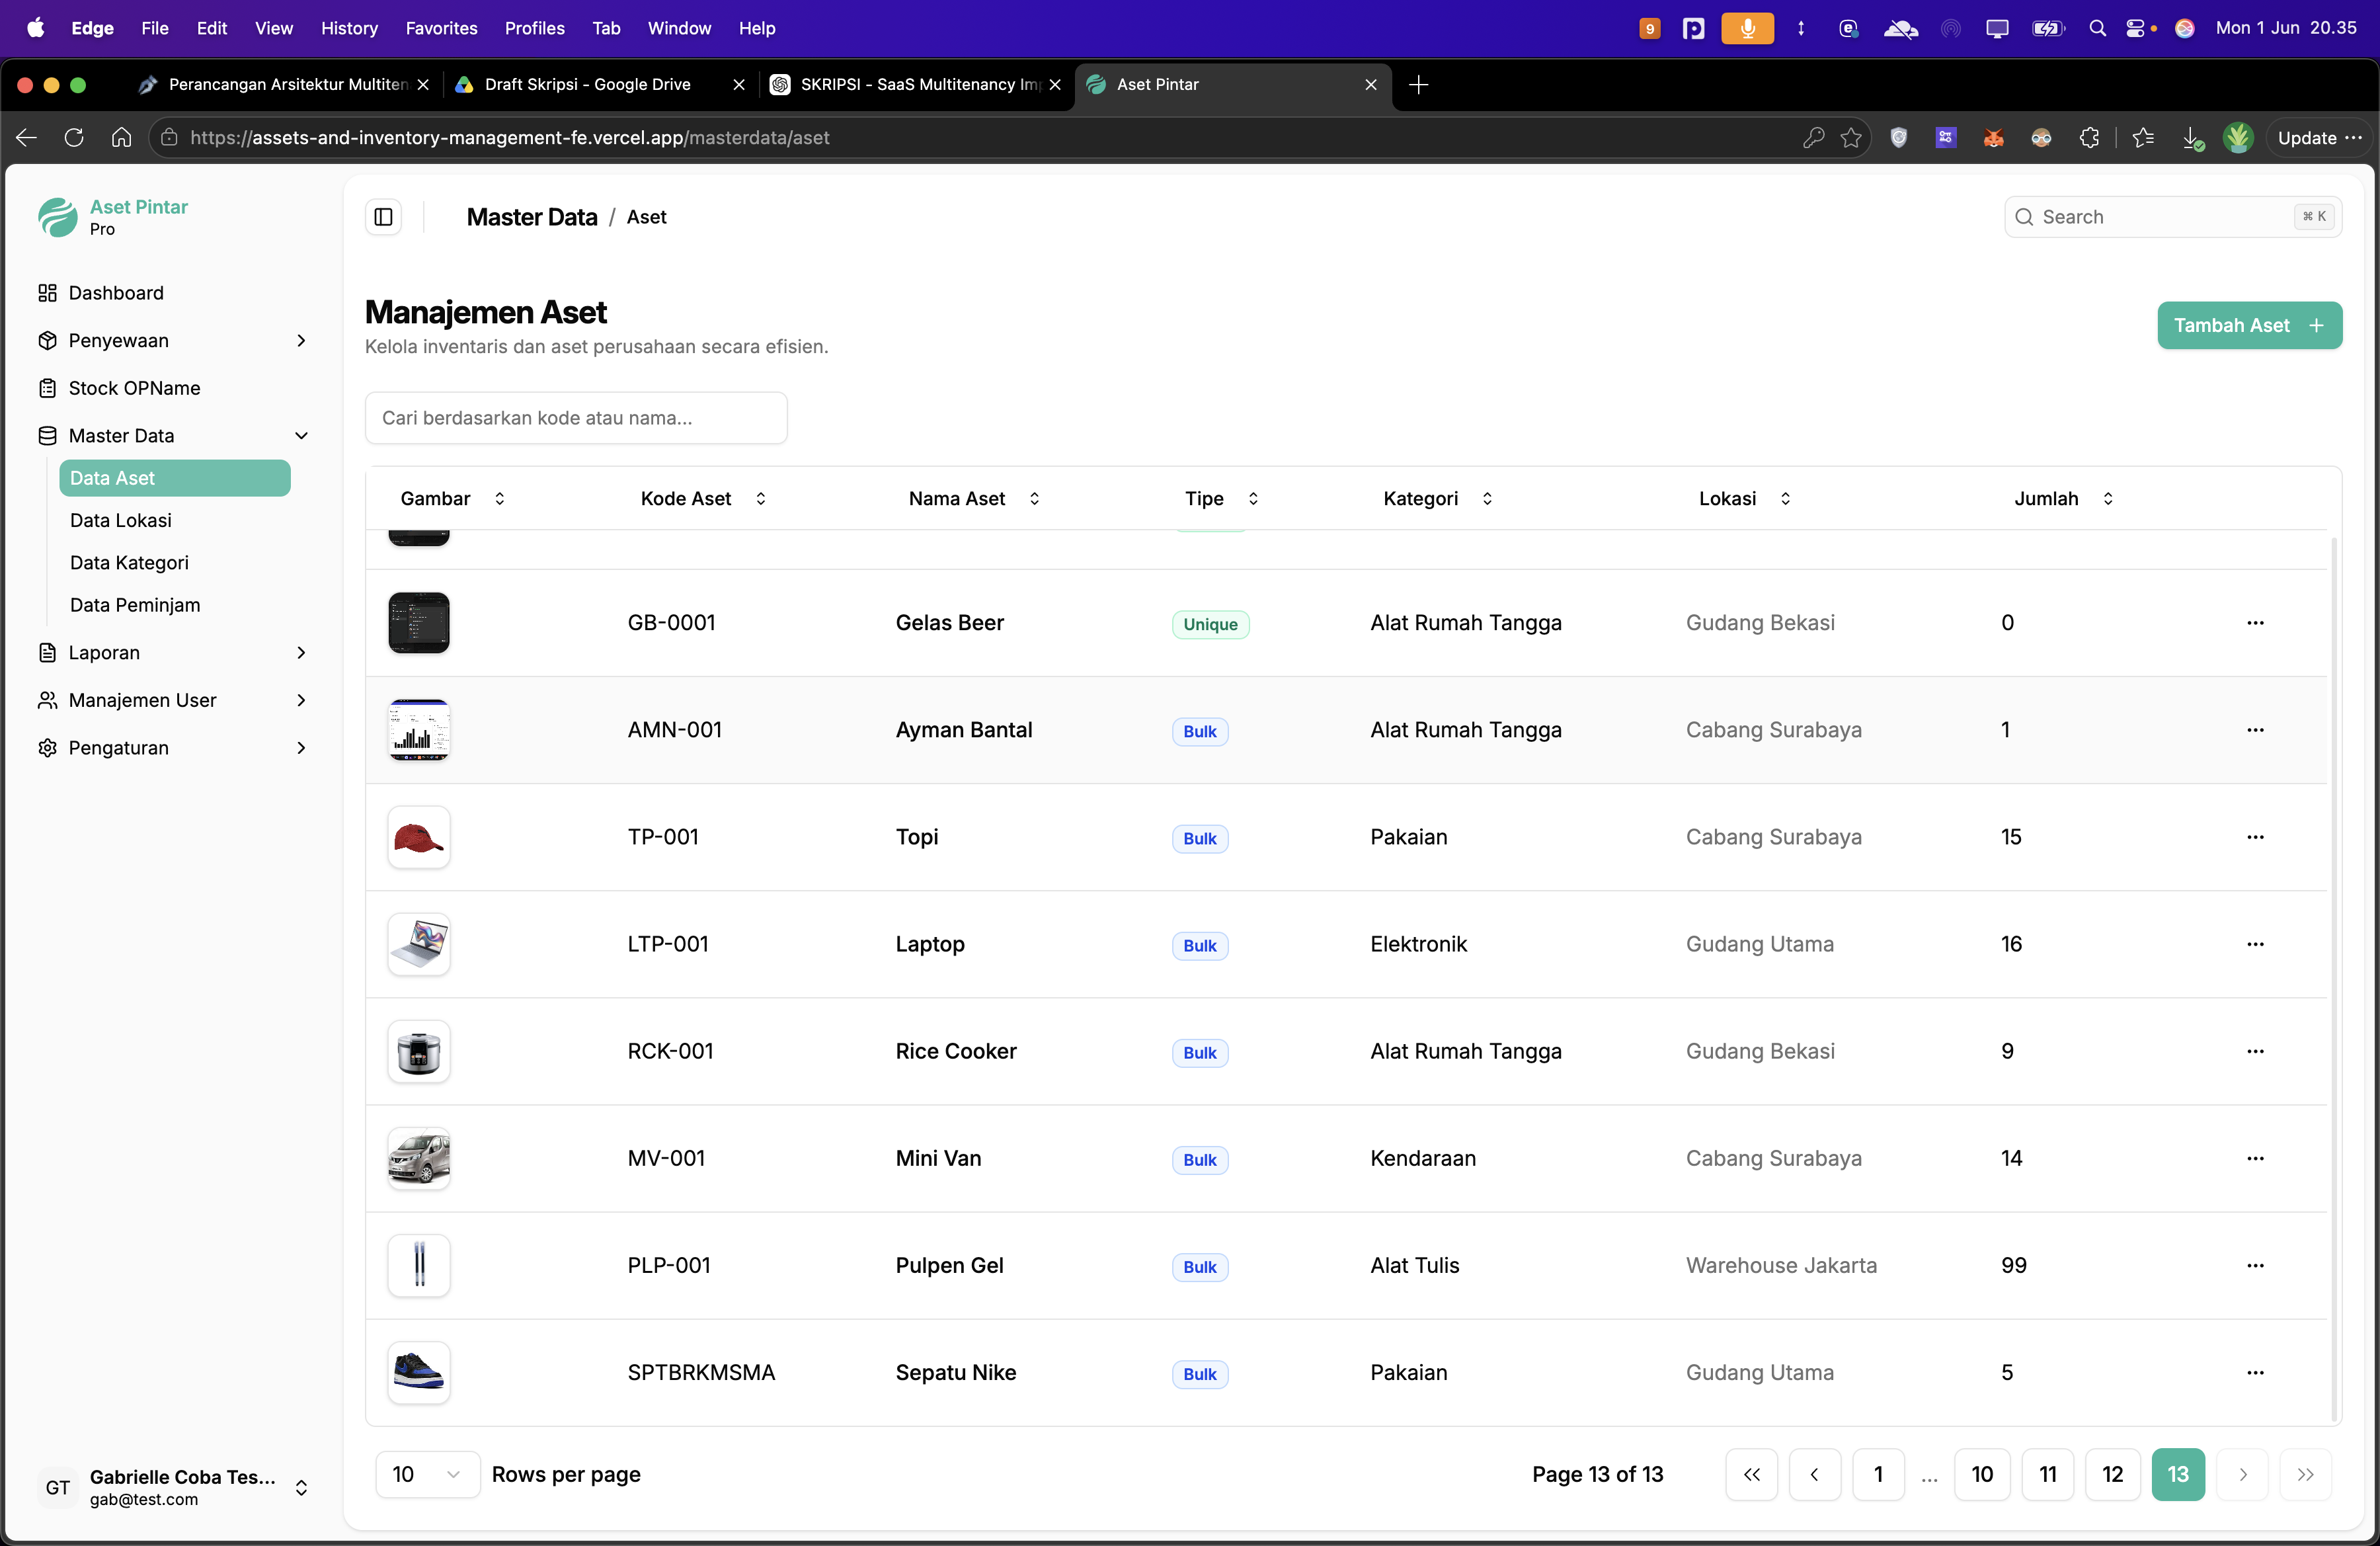
\includegraphics[width=0.9\textwidth]{assets/bab4/test1/web1.png}
  \caption{Data Aset Tenant A pada Aplikasi}
  \label{fig:data_aset_tenant_a}
\end{figure}

Berdasarkan Gambar \ref{fig:data_aset_tenant_a}, pengguna dengan akun \textbf{gab@test.com} hanya dapat melihat data aset yang dimiliki oleh Tenant A. Seluruh data yang ditampilkan pada halaman pengelolaan aset berasal dari \textit{tenant} yang sama dengan akun yang digunakan untuk login. Data milik \textit{tenant} lain tidak ditampilkan pada halaman tersebut meskipun tersimpan pada basis data yang sama.

\begin{figure}[H]
  \centering
  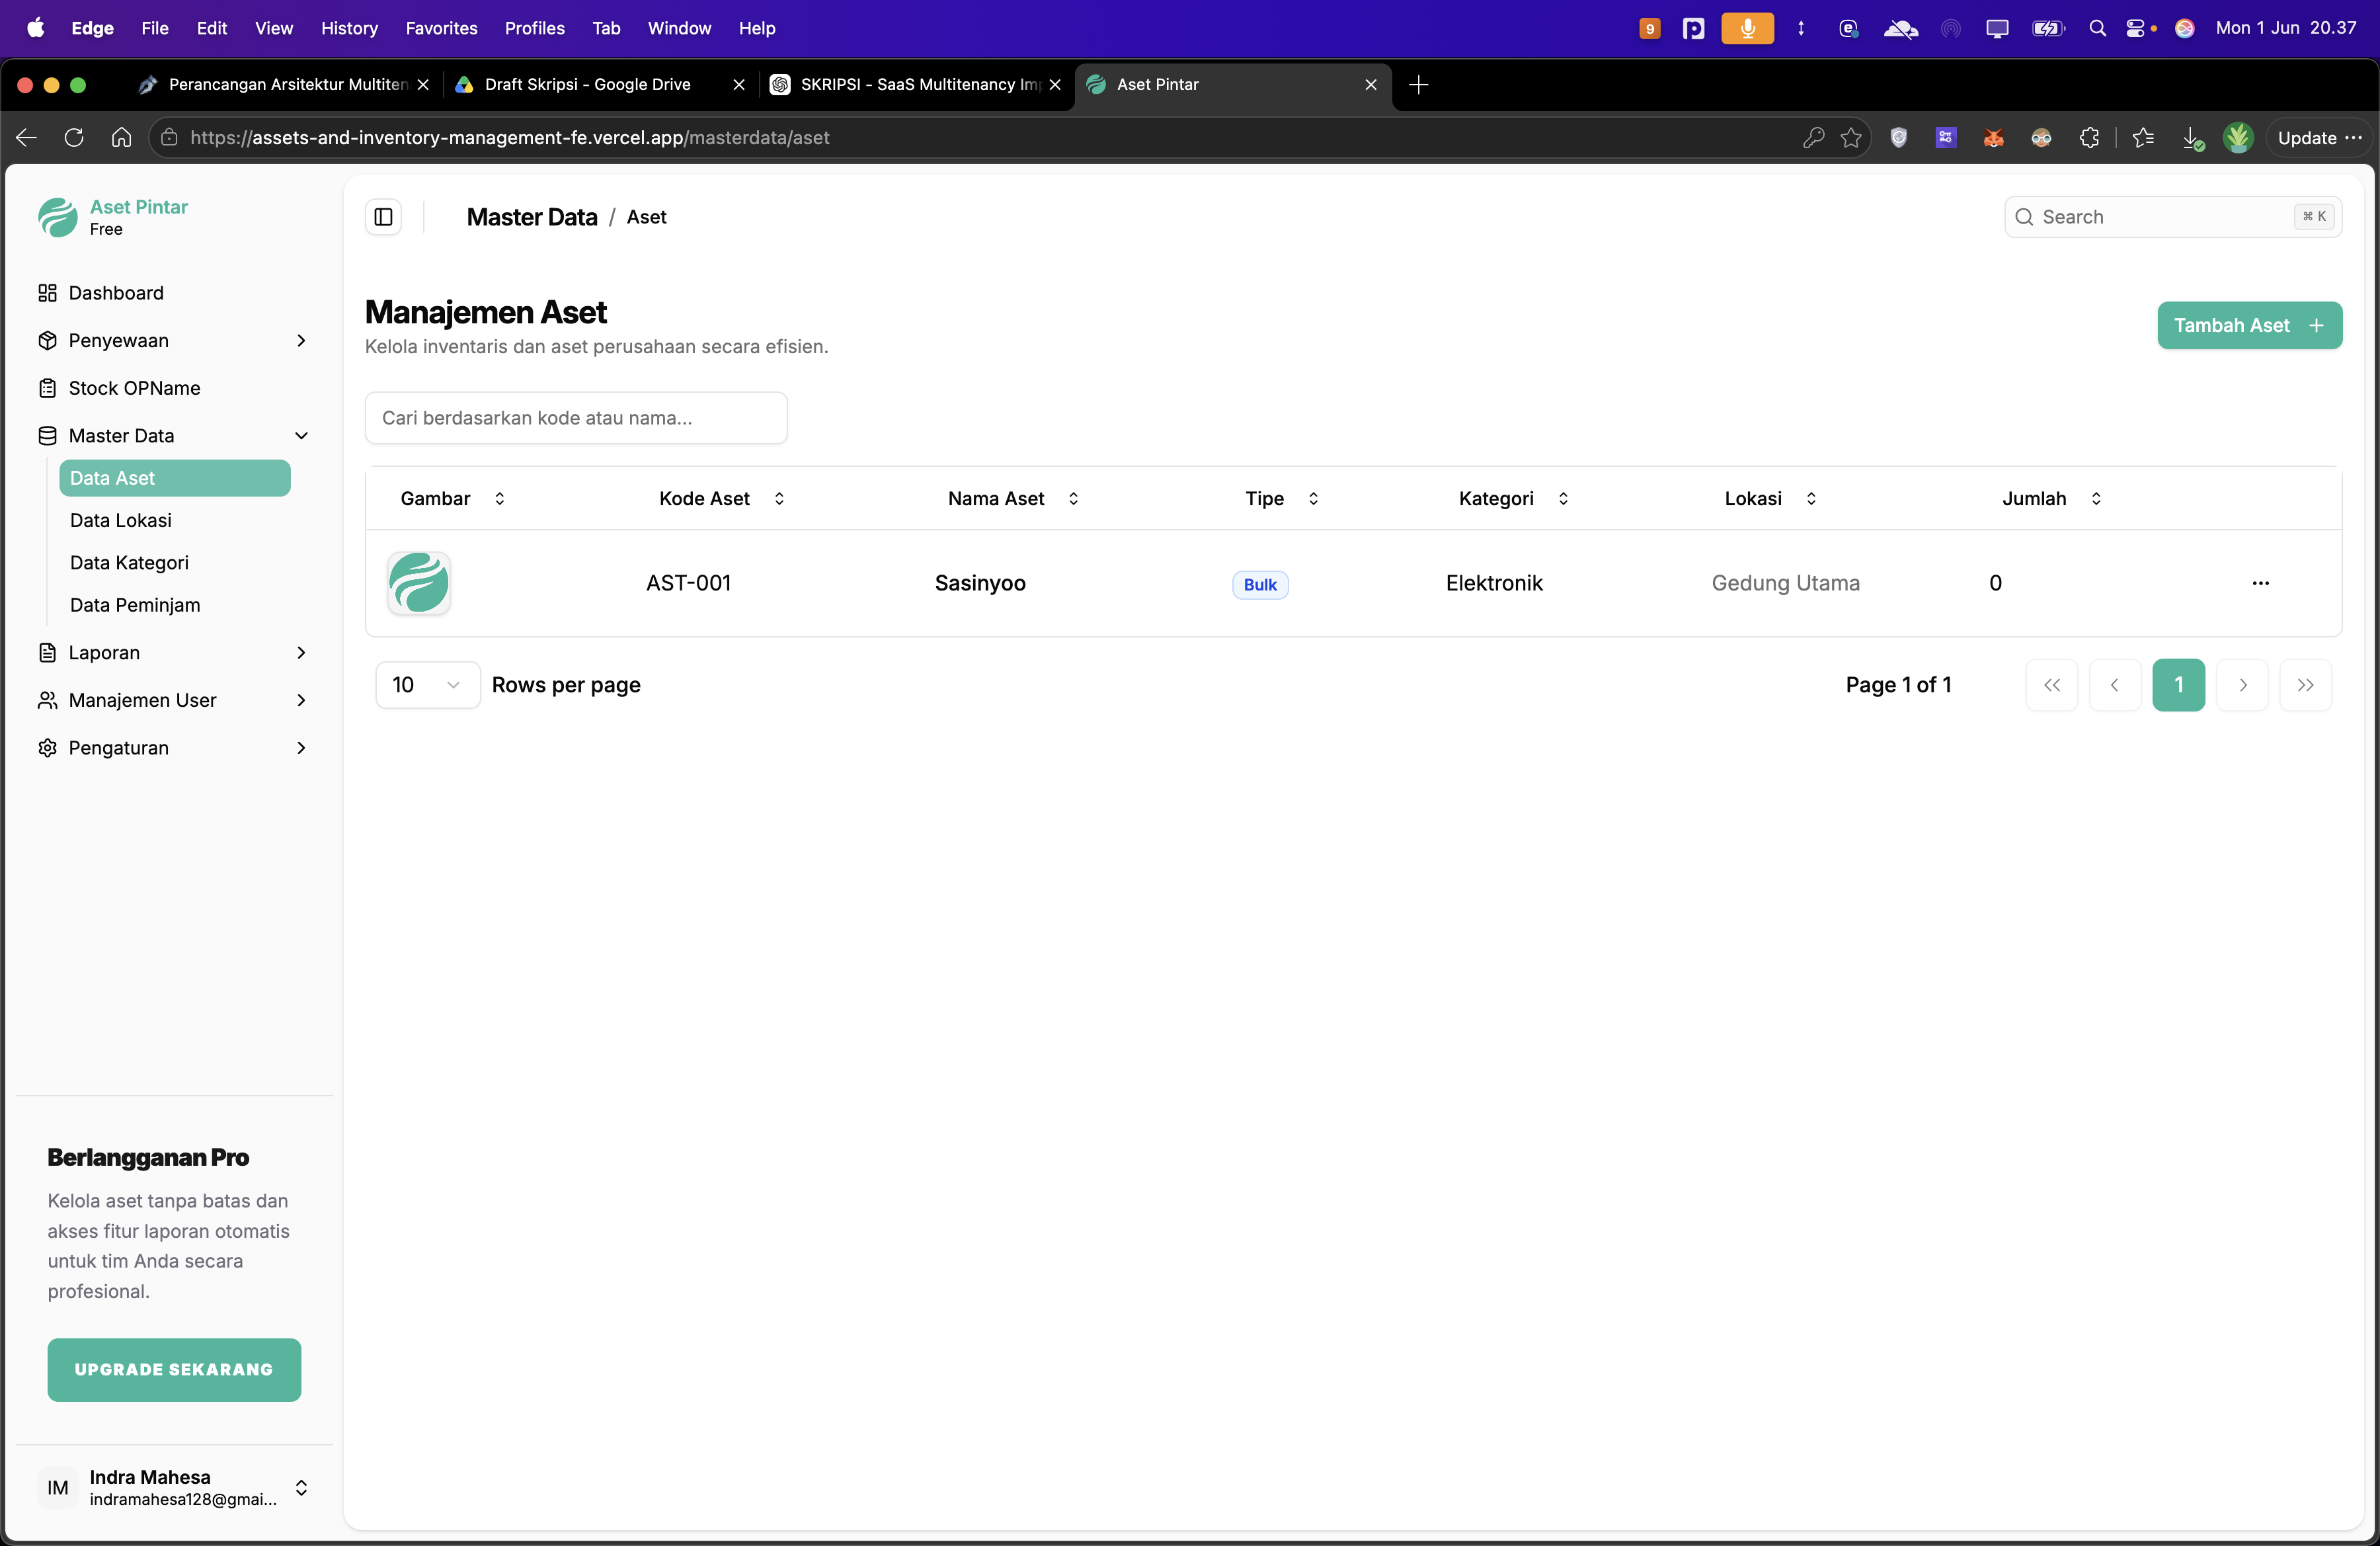
\includegraphics[width=0.9\textwidth]{assets/bab4/test1/web2.png}
  \caption{Data Aset Tenant B pada Aplikasi}
  \label{fig:data_aset_tenant_b}
\end{figure}

Hasil pengujian pada Gambar \ref{fig:data_aset_tenant_b} menunjukkan bahwa pengguna dengan akun \textbf{indramahesa128@gmail.com} hanya dapat mengakses data aset yang dimiliki oleh Tenant B. Data yang ditampilkan berbeda dengan data yang diperoleh oleh Tenant A. Hal tersebut menunjukkan bahwa sistem berhasil menerapkan pemfilteran data berdasarkan identitas \textit{tenant} yang diperoleh pada saat proses autentikasi.

Untuk memastikan bahwa data kedua \textit{tenant} memang tersimpan pada basis data yang sama, dilakukan pemeriksaan langsung pada tabel \textit{assets}. Hasil pemeriksaan ditunjukkan pada Gambar \ref{fig:data_aset_database}.

\begin{figure}[H]
  \centering
  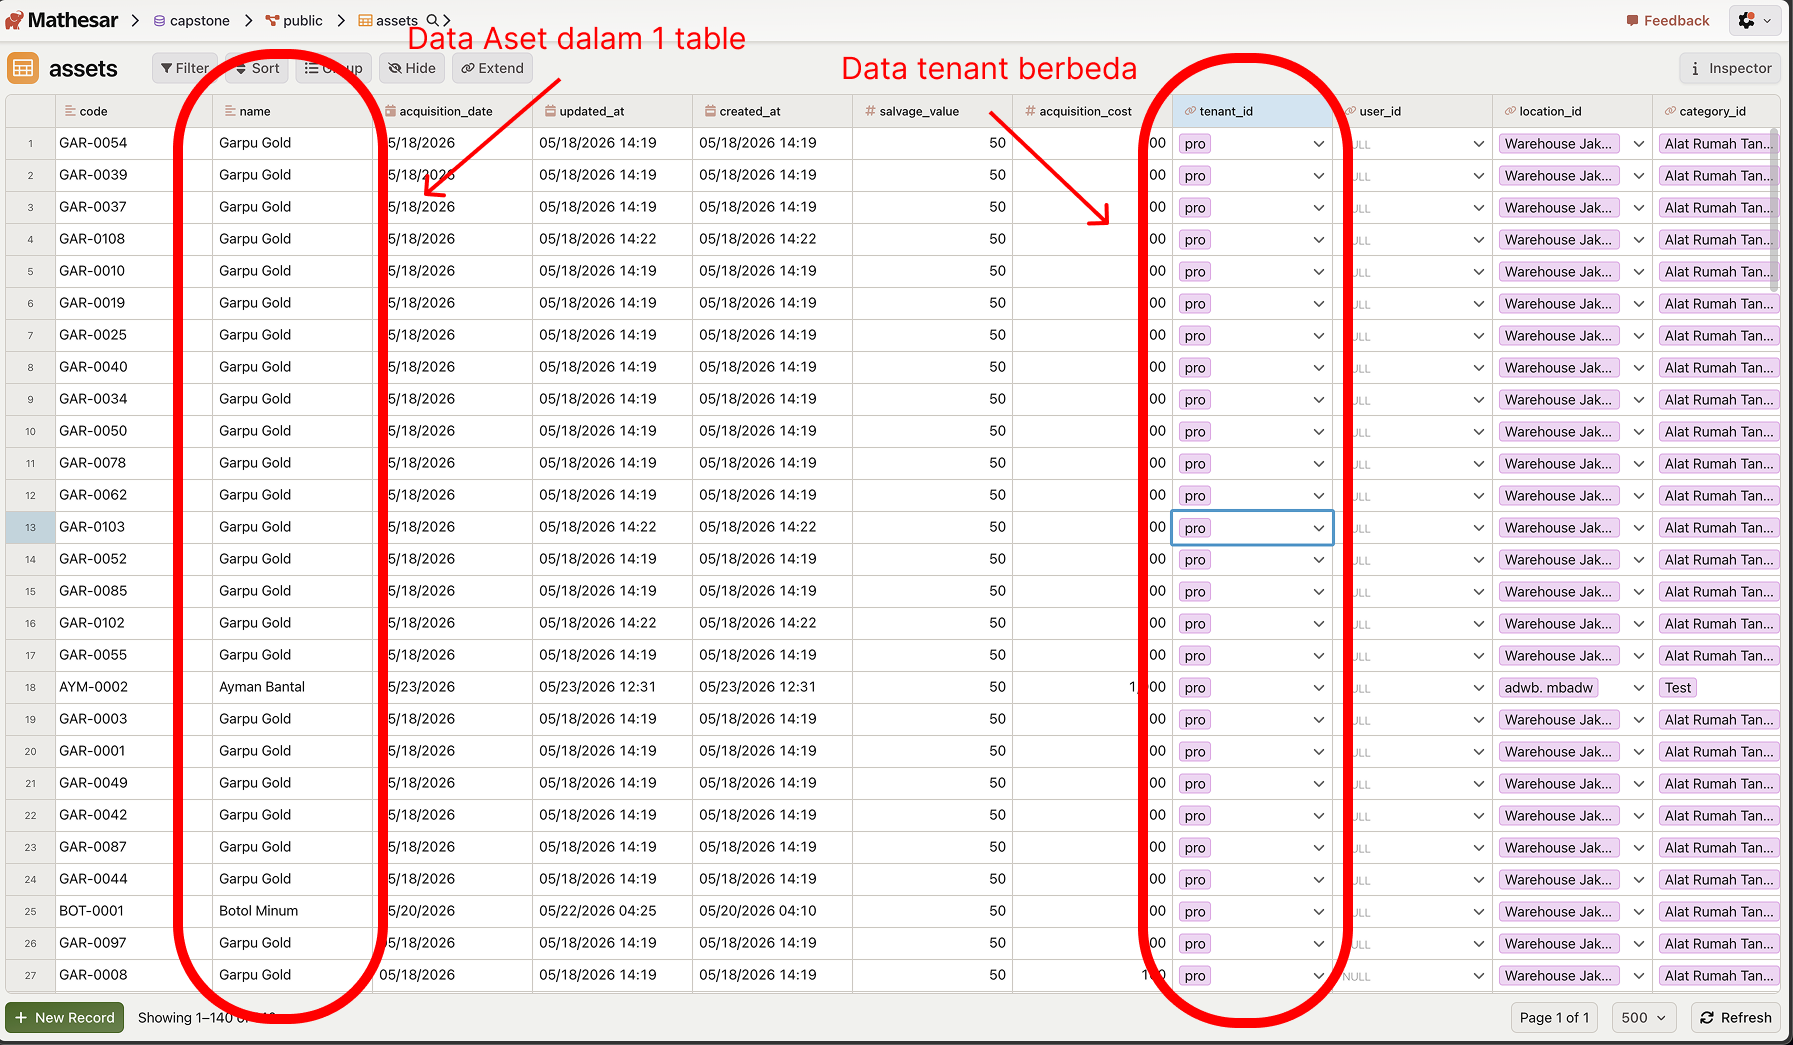
\includegraphics[width=0.9\textwidth]{assets/bab4/test1/db.png}
  \caption{Data Aset Beberapa \textit{Tenant} pada Tabel \textit{Assets}}
  \label{fig:data_aset_database}
\end{figure}

Berdasarkan Gambar \ref{fig:data_aset_database}, data aset dari Tenant A dan Tenant B tersimpan pada tabel \textit{assets} yang sama. Setiap data memiliki atribut \textit{tenant\_id} yang digunakan sebagai identitas kepemilikan data. Atribut tersebut menjadi dasar bagi sistem untuk menentukan data mana yang dapat diakses oleh \textit{tenant} yang sedang aktif. Dengan demikian, meskipun seluruh \textit{tenant} menggunakan tabel yang sama, sistem tetap mampu menjaga pemisahan data antar \textit{tenant}.

Selain melalui antarmuka aplikasi, verifikasi juga dilakukan pada lapisan layanan API. Pengujian ini bertujuan untuk memastikan bahwa mekanisme \textit{tenant isolation} diterapkan secara konsisten pada seluruh lapisan sistem dan tidak hanya pada tampilan aplikasi.

\begin{figure}[H]
  \centering
  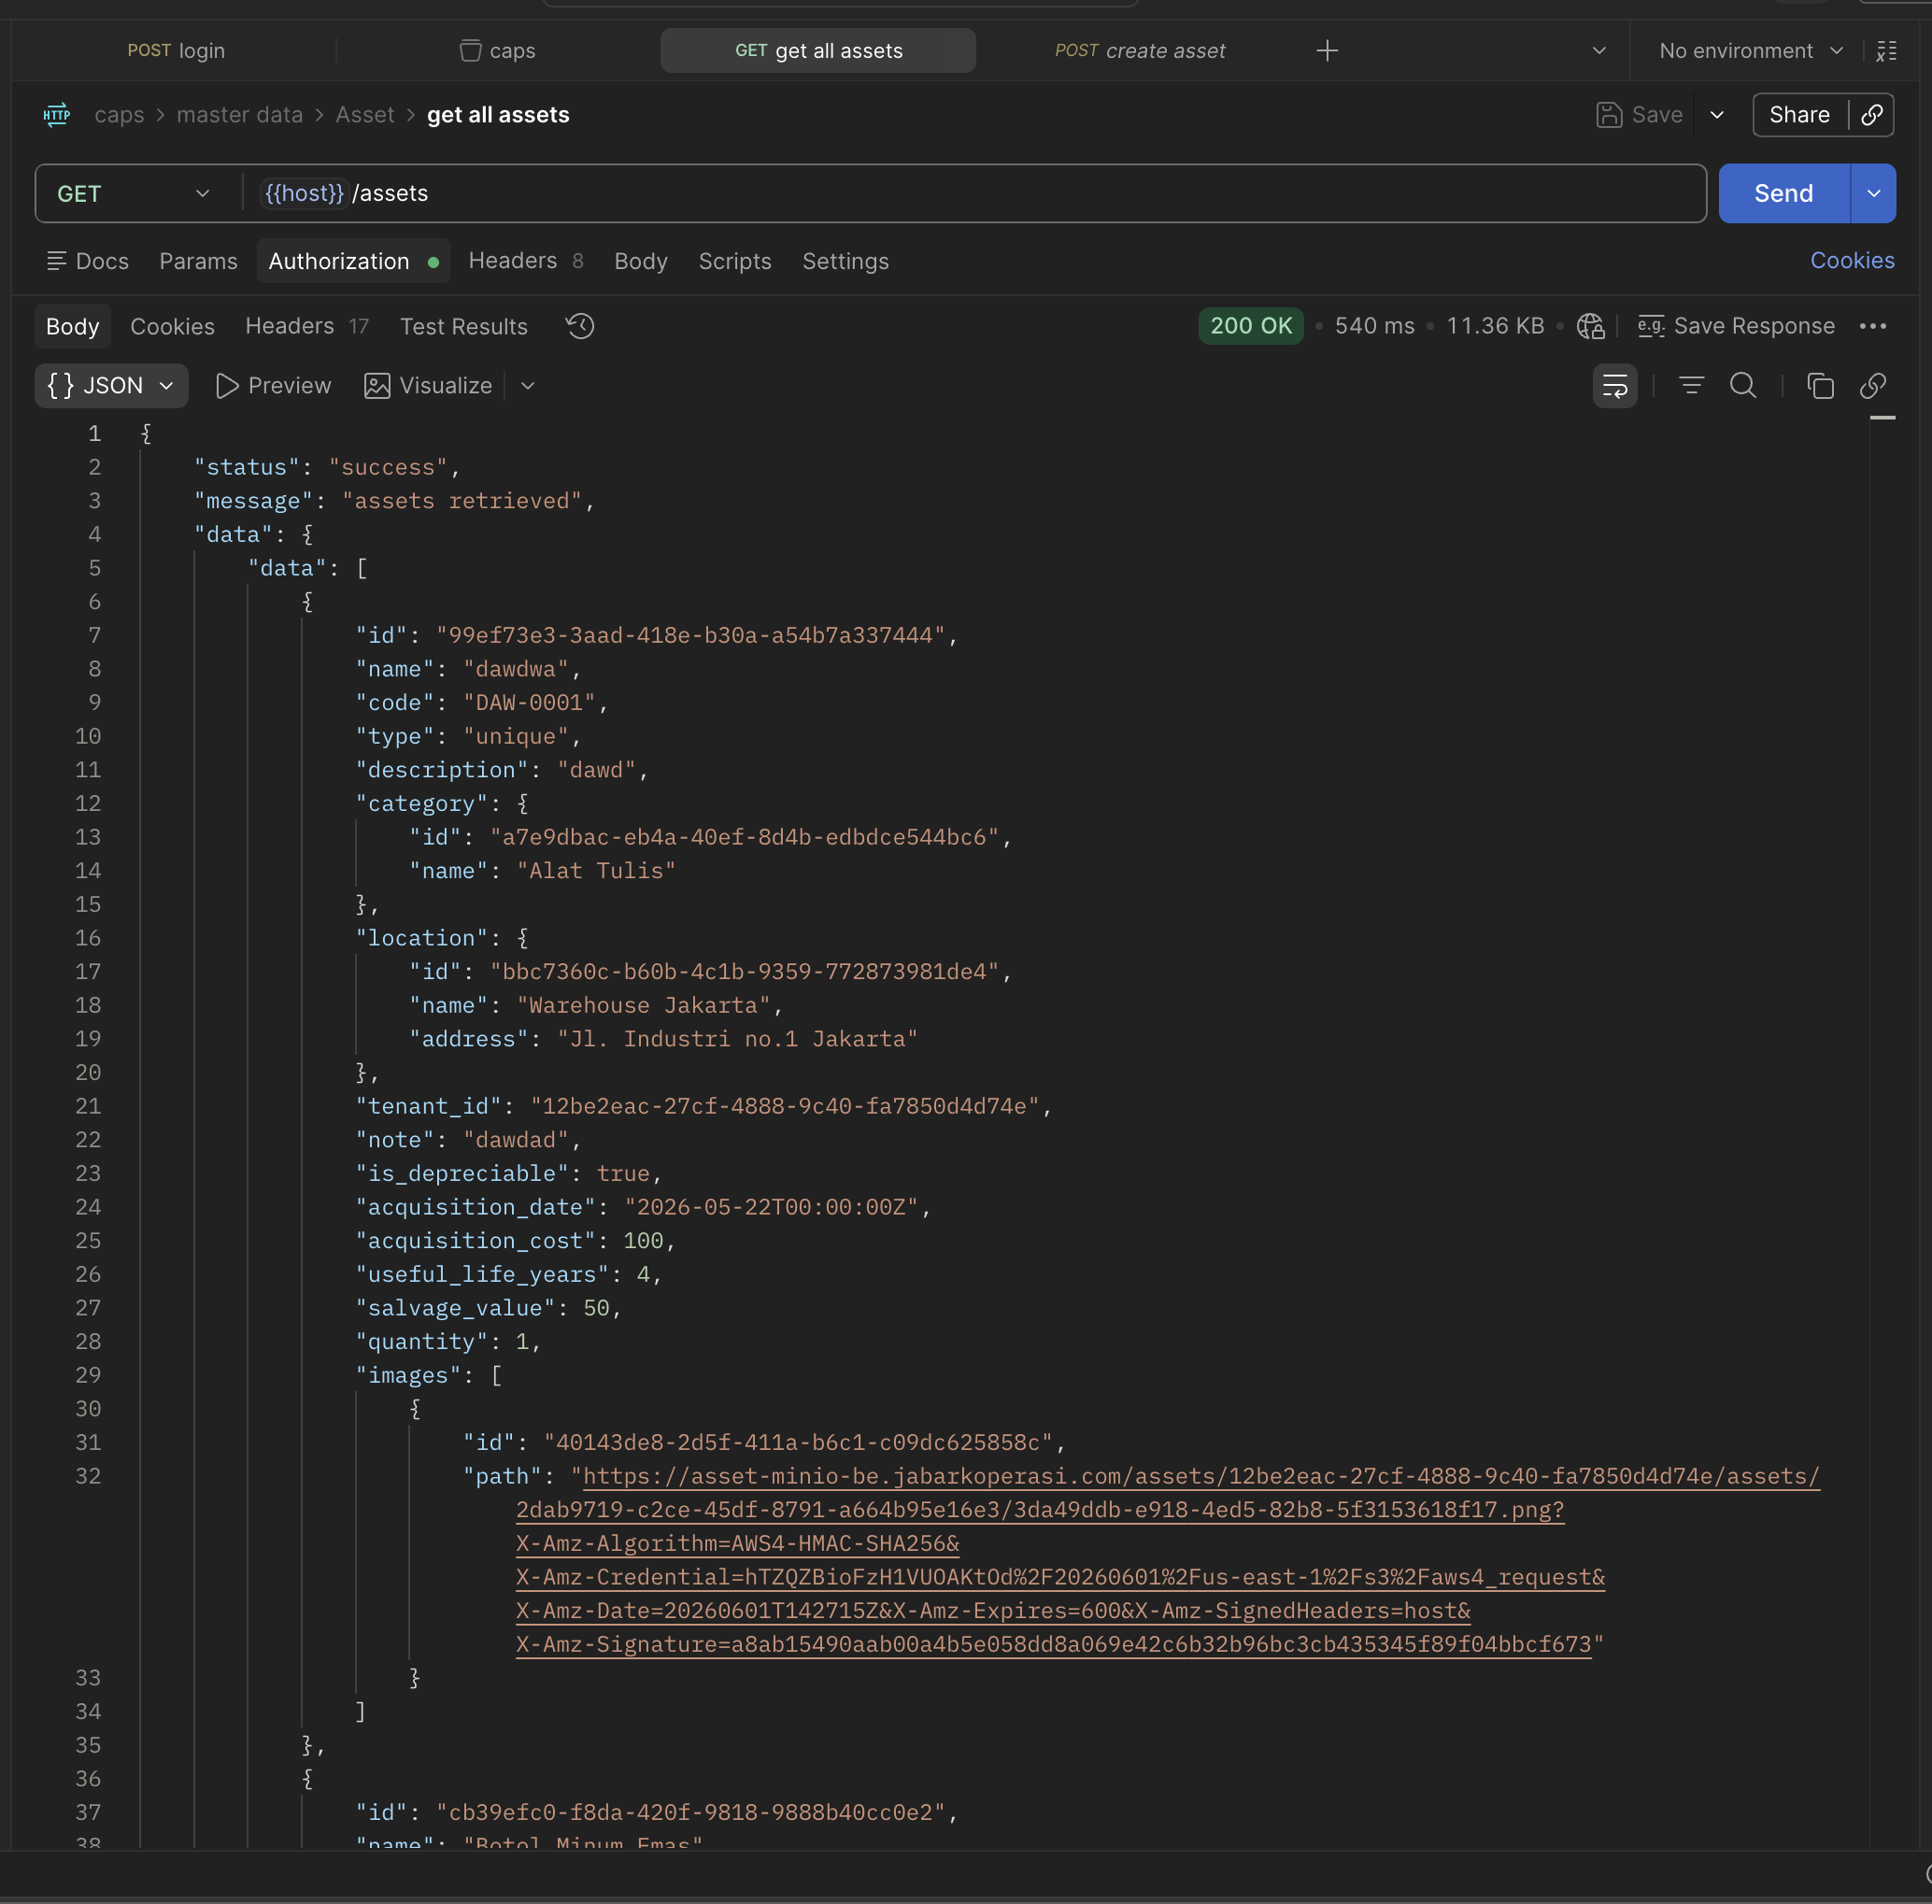
\includegraphics[width=0.9\textwidth]{assets/bab4/test1/api1.png}
  \caption{Respons API Pengambilan Data Aset Tenant A}
  \label{fig:api_tenant_a}
\end{figure}

Berdasarkan Gambar \ref{fig:api_tenant_a}, layanan API hanya mengembalikan data aset yang dimiliki Tenant A. Data yang berasal dari Tenant B tidak terdapat pada respons yang diterima pengguna. Hasil tersebut menunjukkan bahwa identitas \textit{tenant} yang tersimpan pada token autentikasi berhasil digunakan sebagai parameter pembatas akses data.

\begin{figure}[H]
  \centering
  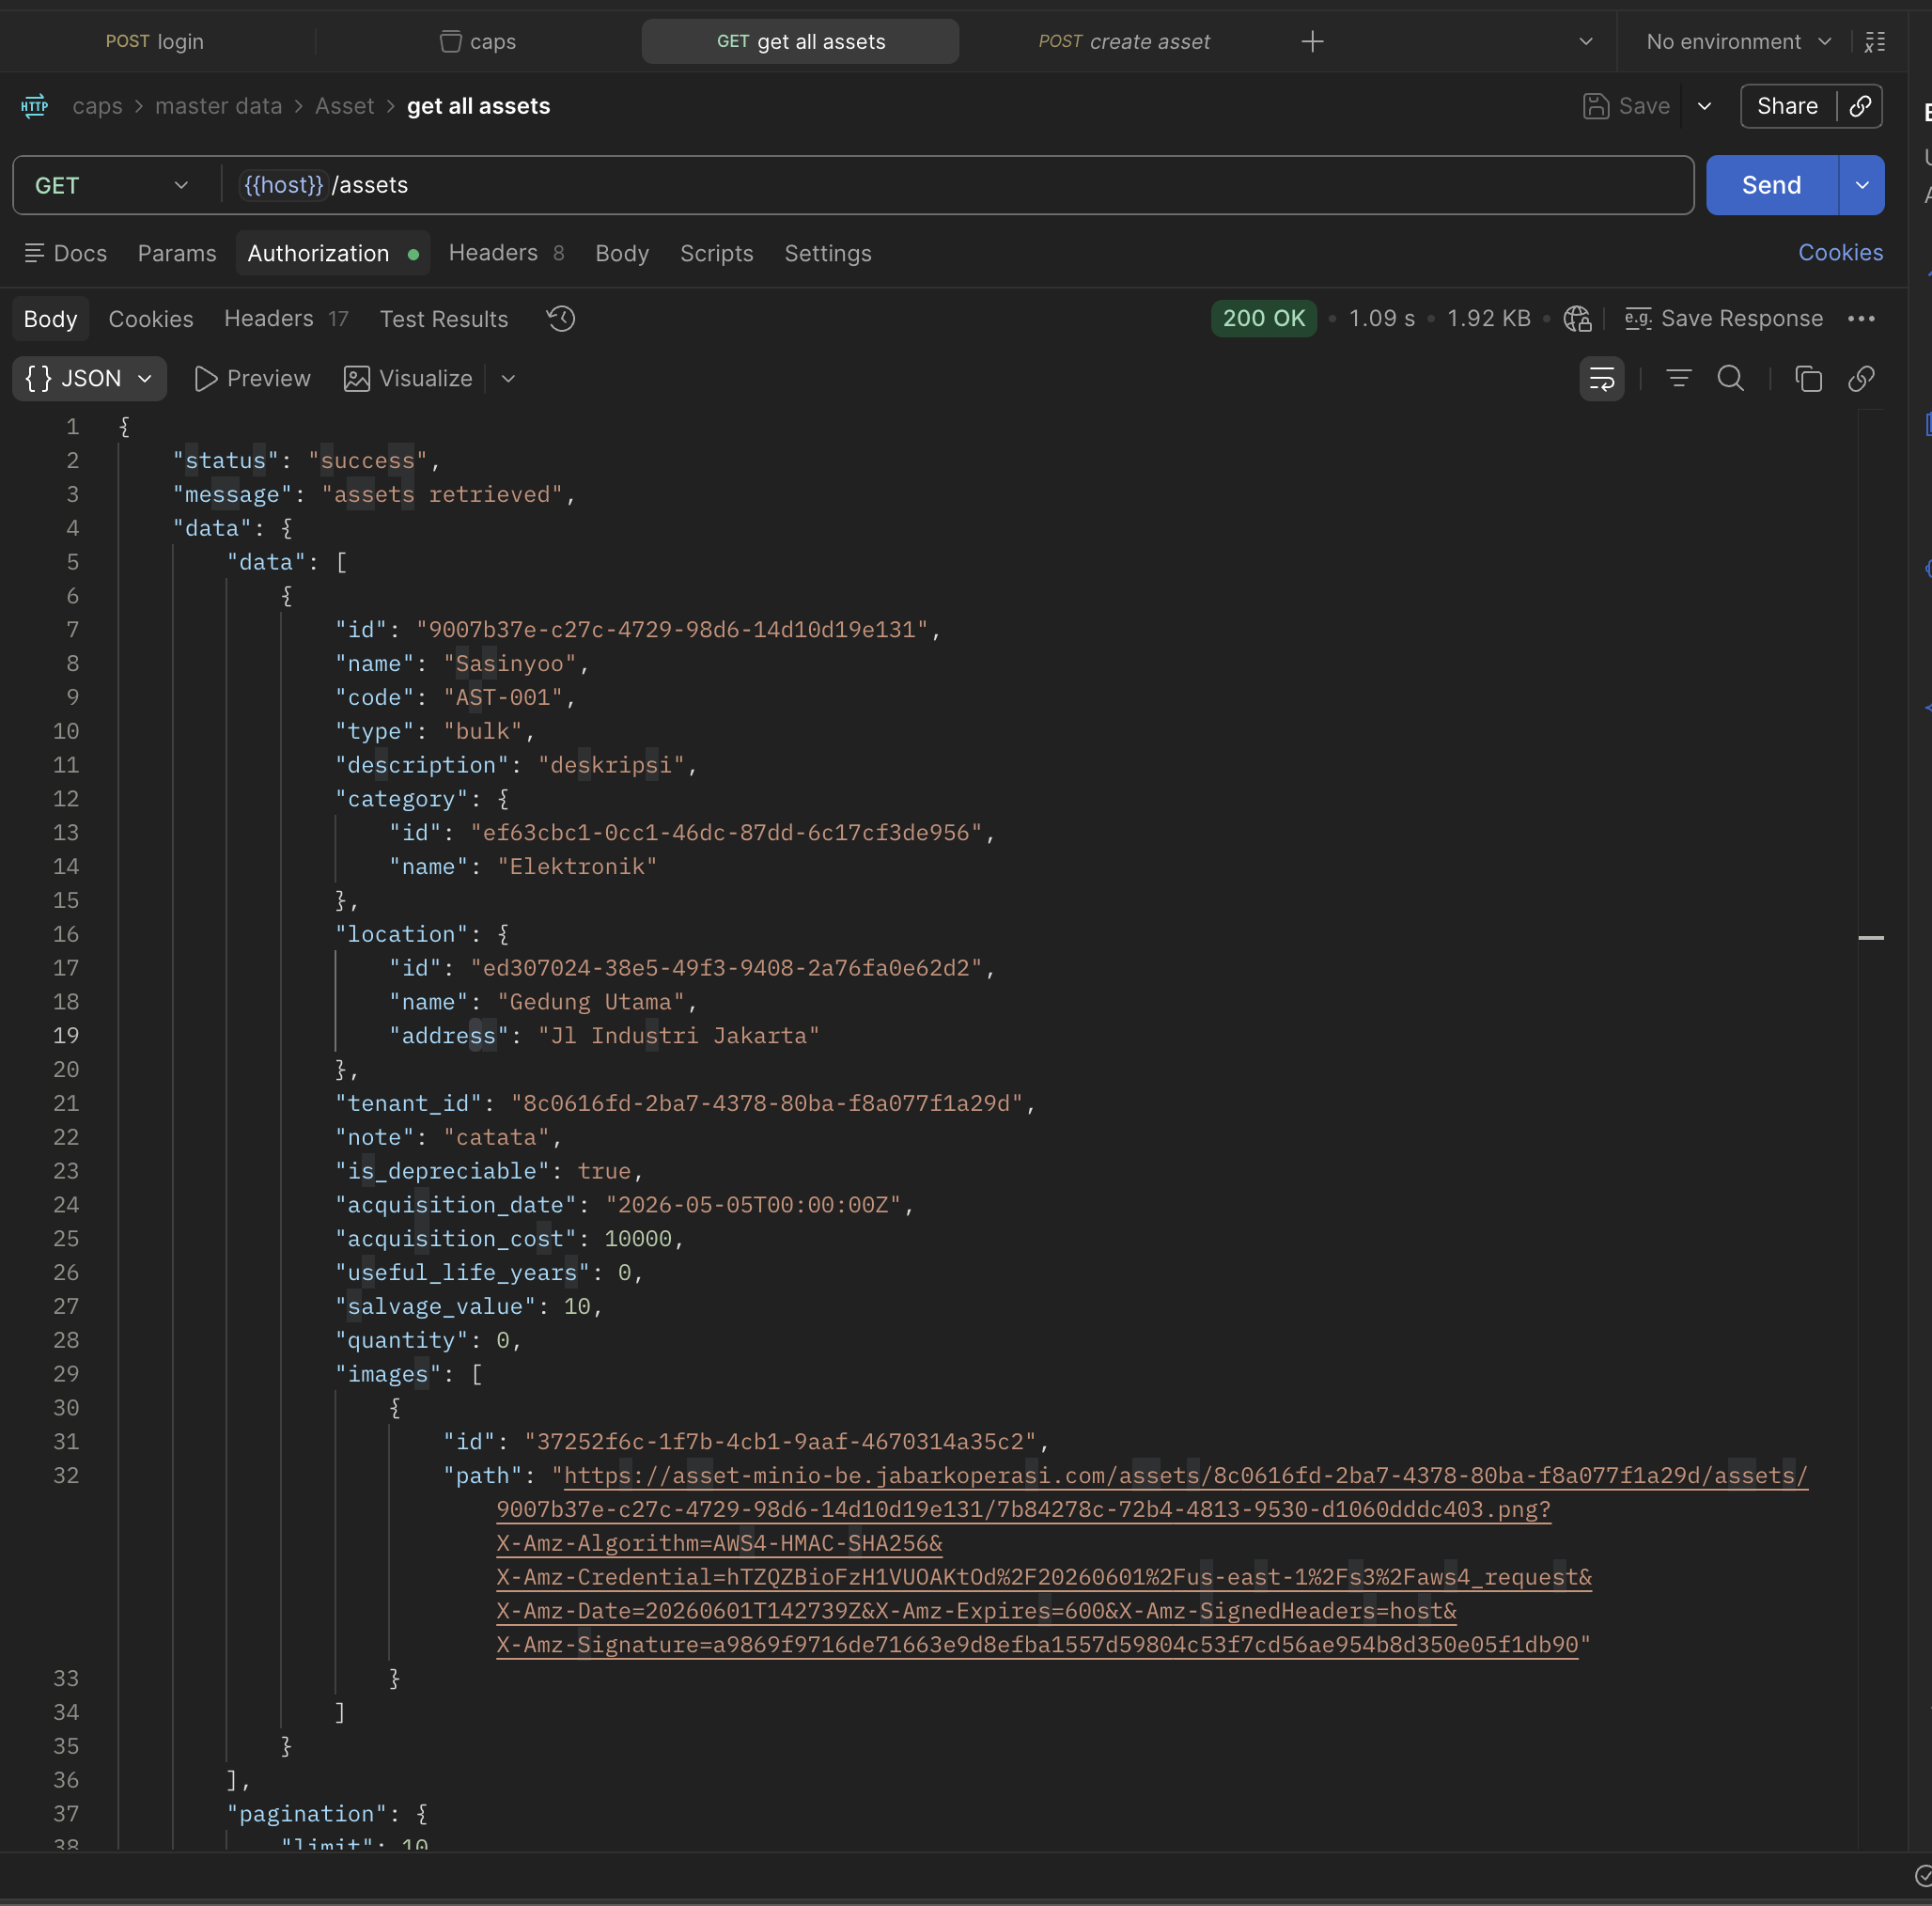
\includegraphics[width=0.9\textwidth]{assets/bab4/test1/api2.png}
  \caption{Respons API Pengambilan Data Aset Tenant B}
  \label{fig:api_tenant_b}
\end{figure}

Hasil yang ditunjukkan pada Gambar \ref{fig:api_tenant_b} memperlihatkan bahwa pengguna Tenant B memperoleh data yang berbeda dengan Tenant A. Sistem hanya mengembalikan data yang memiliki keterkaitan dengan \textit{tenant} yang sedang aktif. Dengan demikian, akses terhadap data \textit{tenant} lain dapat dicegah meskipun permintaan dilakukan melalui \textit{endpoint} API yang sama.

Untuk mempermudah evaluasi hasil pengujian, ringkasan hasil pengujian \textit{tenant isolation} disajikan pada Tabel \ref{tab:hasil_pengujian_tenant_isolation}.

\begin{table}[H]
  \centering
  \caption{Hasil Pengujian \textit{Tenant Isolation}}
  \label{tab:hasil_pengujian_tenant_isolation}
  \footnotesize
  \begin{tabular}{|c|p{5cm}|p{4cm}|p{2.5cm}|}
    \hline
    \rowcolor[HTML]{EFEFEF}
    \textbf{No} & \textbf{Skenario Pengujian} & \textbf{Hasil yang Diharapkan} & \textbf{Hasil Pengujian} \\
    \hline
    1 & Tenant A mengakses data aset Tenant A & Data berhasil ditampilkan & Berhasil \\
    \hline
    2 & Tenant B mengakses data aset Tenant B & Data berhasil ditampilkan & Berhasil \\
    \hline
    3 & Tenant A mencoba mengakses data Tenant B & Data tidak ditampilkan & Berhasil \\
    \hline
    4 & Tenant B mencoba mengakses data Tenant A & Data tidak ditampilkan & Berhasil \\
    \hline
    5 & \textit{Tenant} melakukan perubahan data aset & Perubahan hanya berlaku pada data \textit{tenant} terkait & Berhasil \\
    \hline
  \end{tabular}
\end{table}

Berdasarkan hasil pengujian pada Tabel \ref{tab:hasil_pengujian_tenant_isolation}, seluruh skenario pengujian berhasil dijalankan sesuai dengan hasil yang diharapkan. Pengguna hanya dapat mengakses data yang berada dalam ruang lingkup \textit{tenant} yang sesuai, baik melalui antarmuka aplikasi maupun layanan API. Selain itu, pemeriksaan pada basis data menunjukkan bahwa data dari beberapa \textit{tenant} dapat disimpan pada tabel yang sama tanpa menyebabkan pencampuran data.

Hasil tersebut menunjukkan bahwa mekanisme \textit{tenant isolation} yang dirancang pada penelitian ini berhasil diterapkan pada lapisan aplikasi, layanan API, dan basis data. Dengan demikian, pendekatan \textit{shared database} dan \textit{shared schema} yang digunakan tetap mampu menjaga pemisahan data antar \textit{tenant} sesuai dengan tujuan penelitian yang telah ditetapkan.

\subsection{Hasil Pengujian Tenant Provisioning}

Pengujian \textit{tenant provisioning} dilakukan untuk memverifikasi bahwa proses registrasi \textit{tenant} baru dapat berjalan secara otomatis sesuai dengan rancangan yang telah dijelaskan pada Bab 3. Pengujian ini bertujuan untuk memastikan bahwa sistem mampu membuat \textit{tenant} baru beserta seluruh konfigurasi awal yang diperlukan, sehingga \textit{tenant} dapat langsung menggunakan sistem setelah proses registrasi selesai.

Pada pengujian ini, dilakukan registrasi \textit{tenant} baru menggunakan data organisasi dan akun administrator yang belum pernah terdaftar pada sistem. Setelah proses registrasi berhasil dilakukan, verifikasi dilakukan terhadap data \textit{tenant}, \textit{role} administrator, \textit{permission}, serta akun administrator yang terbentuk secara otomatis pada basis data.

\begin{figure}[H]
  \centering
  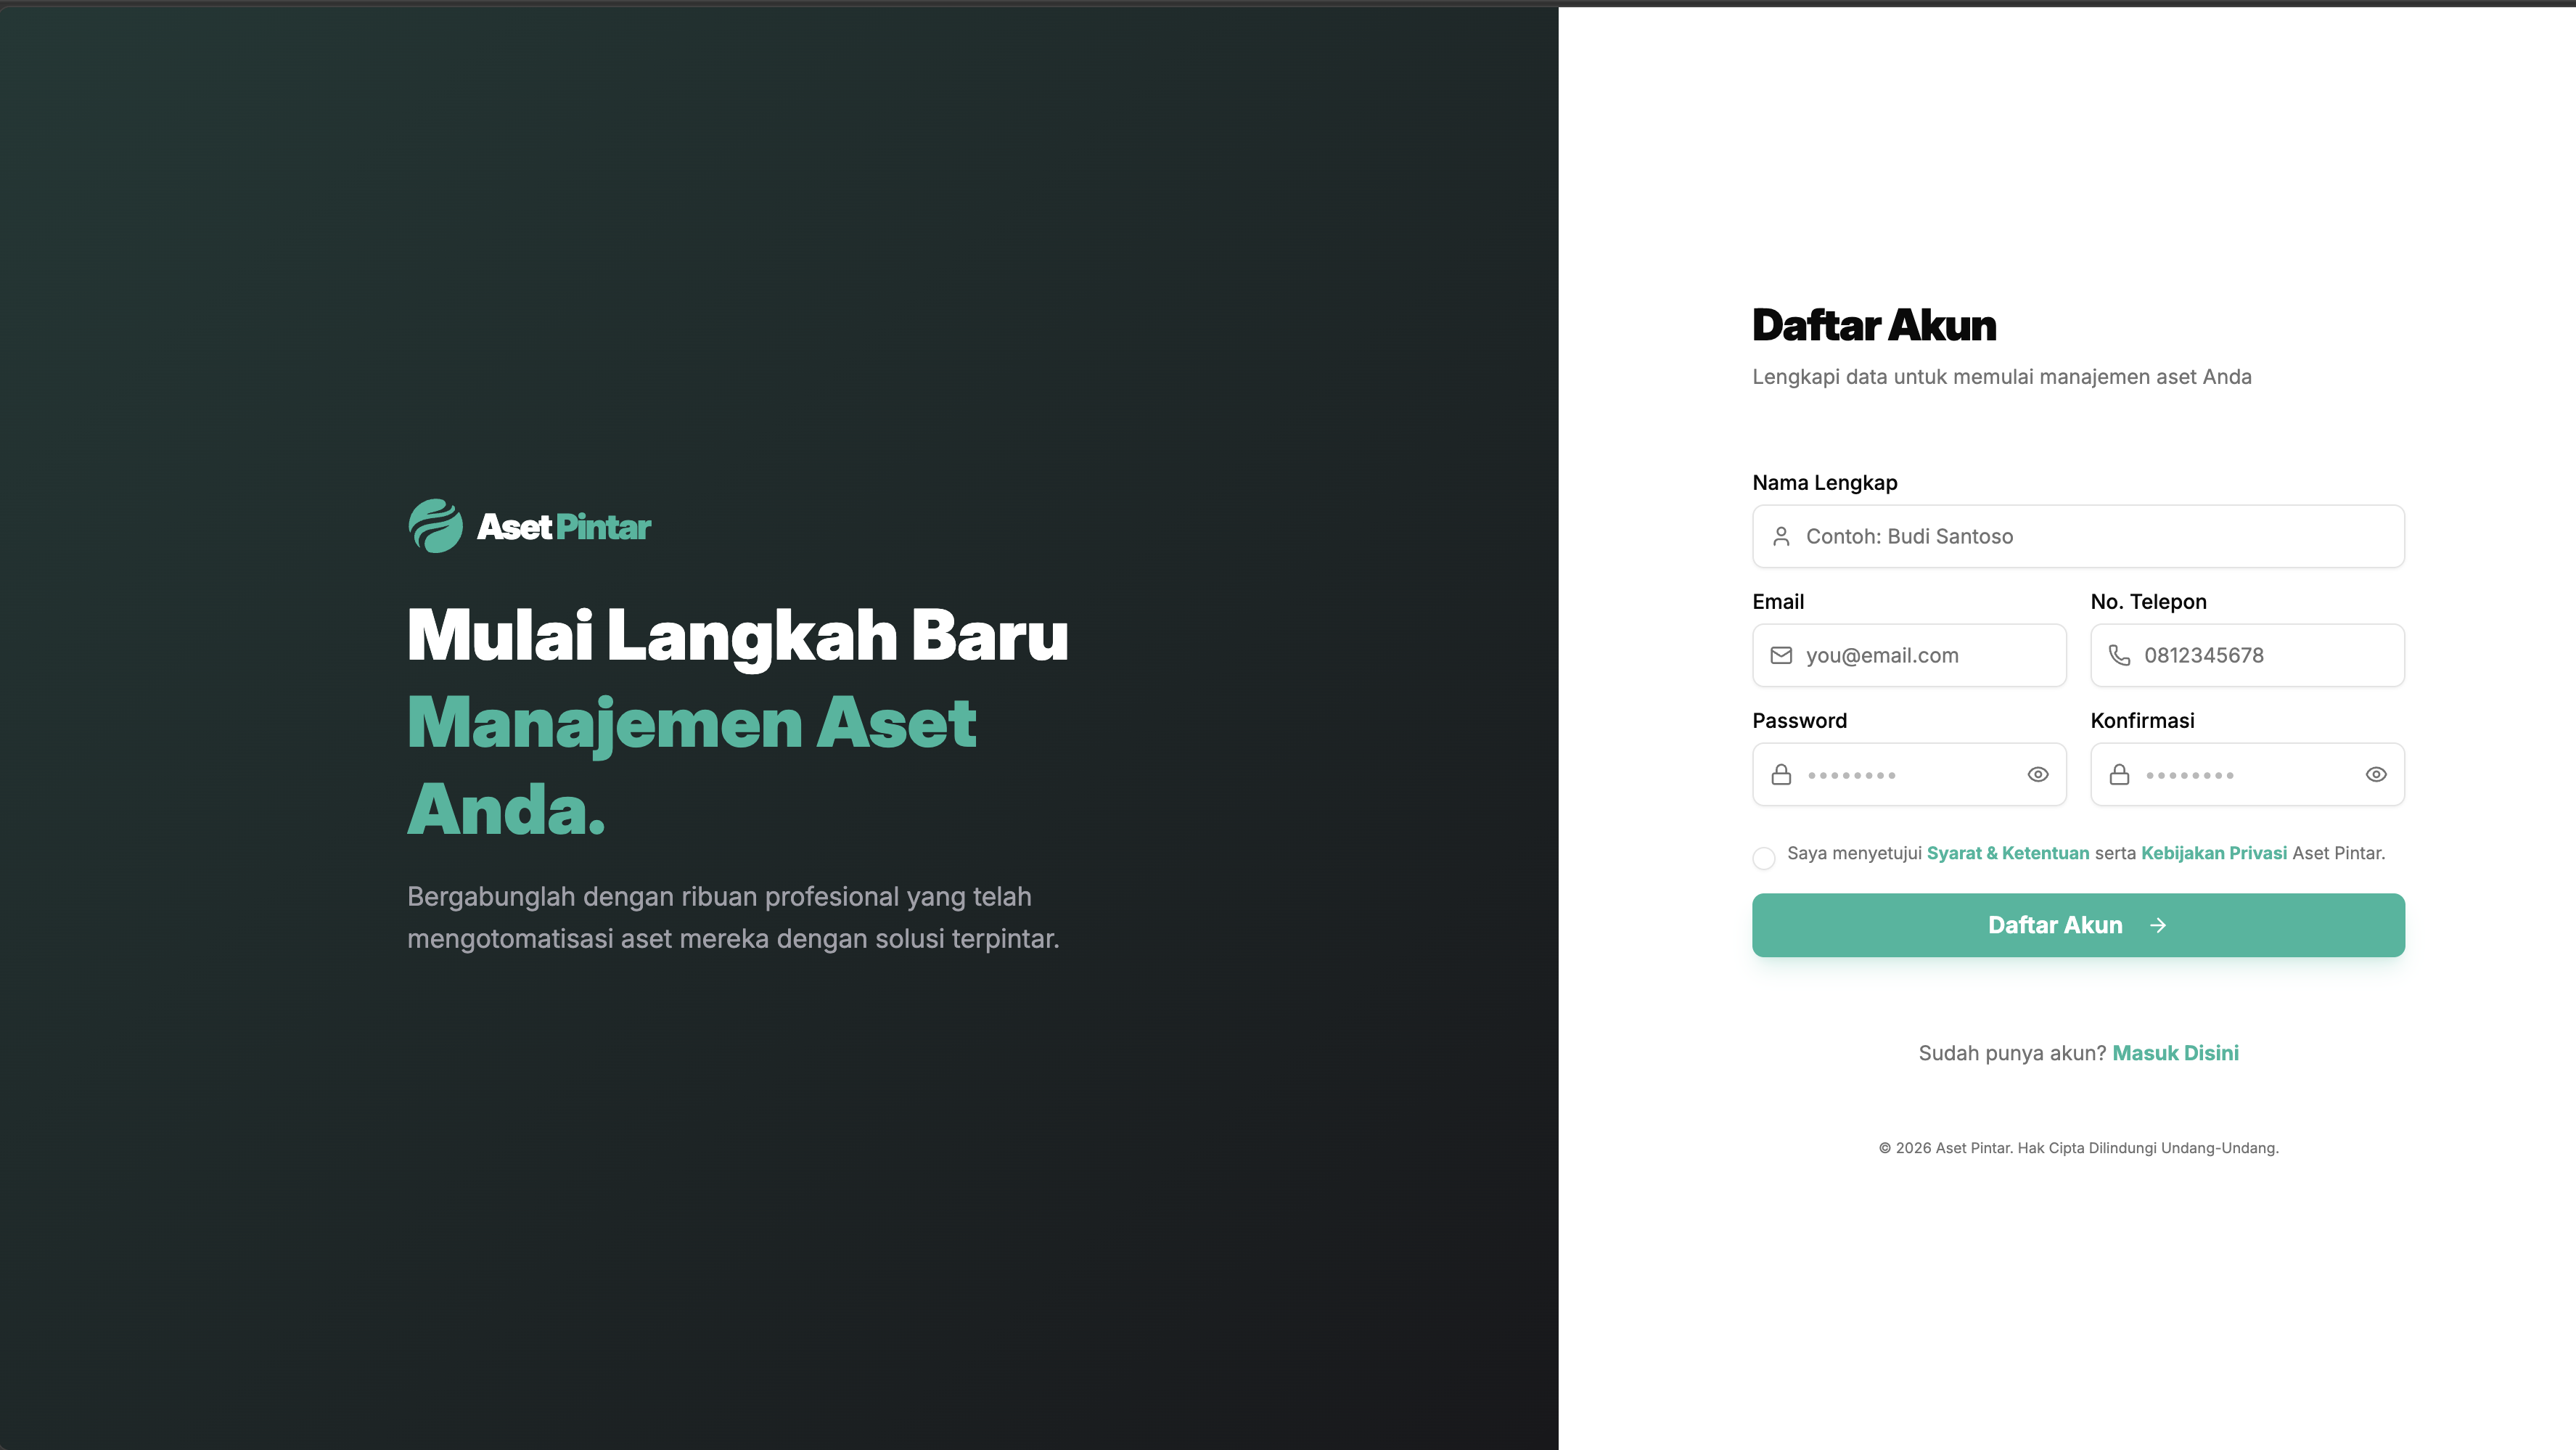
\includegraphics[width=0.9\textwidth]{assets/bab4/test2/signup.png}
  \caption{Form Registrasi \textit{Tenant} Baru}
  \label{fig:form_registrasi_tenant}
\end{figure}

Berdasarkan Gambar \ref{fig:form_registrasi_tenant}, pengguna mengisi informasi yang diperlukan untuk proses registrasi \textit{tenant}. Informasi tersebut mencakup data \textit{tenant} dan akun administrator yang akan digunakan untuk mengakses sistem setelah proses registrasi berhasil dilakukan.

Setelah proses registrasi berhasil dijalankan, sistem secara otomatis membuat data \textit{tenant} baru pada tabel \textit{tenants}. Hasil pembentukan data \textit{tenant} ditunjukkan pada Gambar \ref{fig:data_tenant_baru}.

\begin{figure}[H]
  \centering
  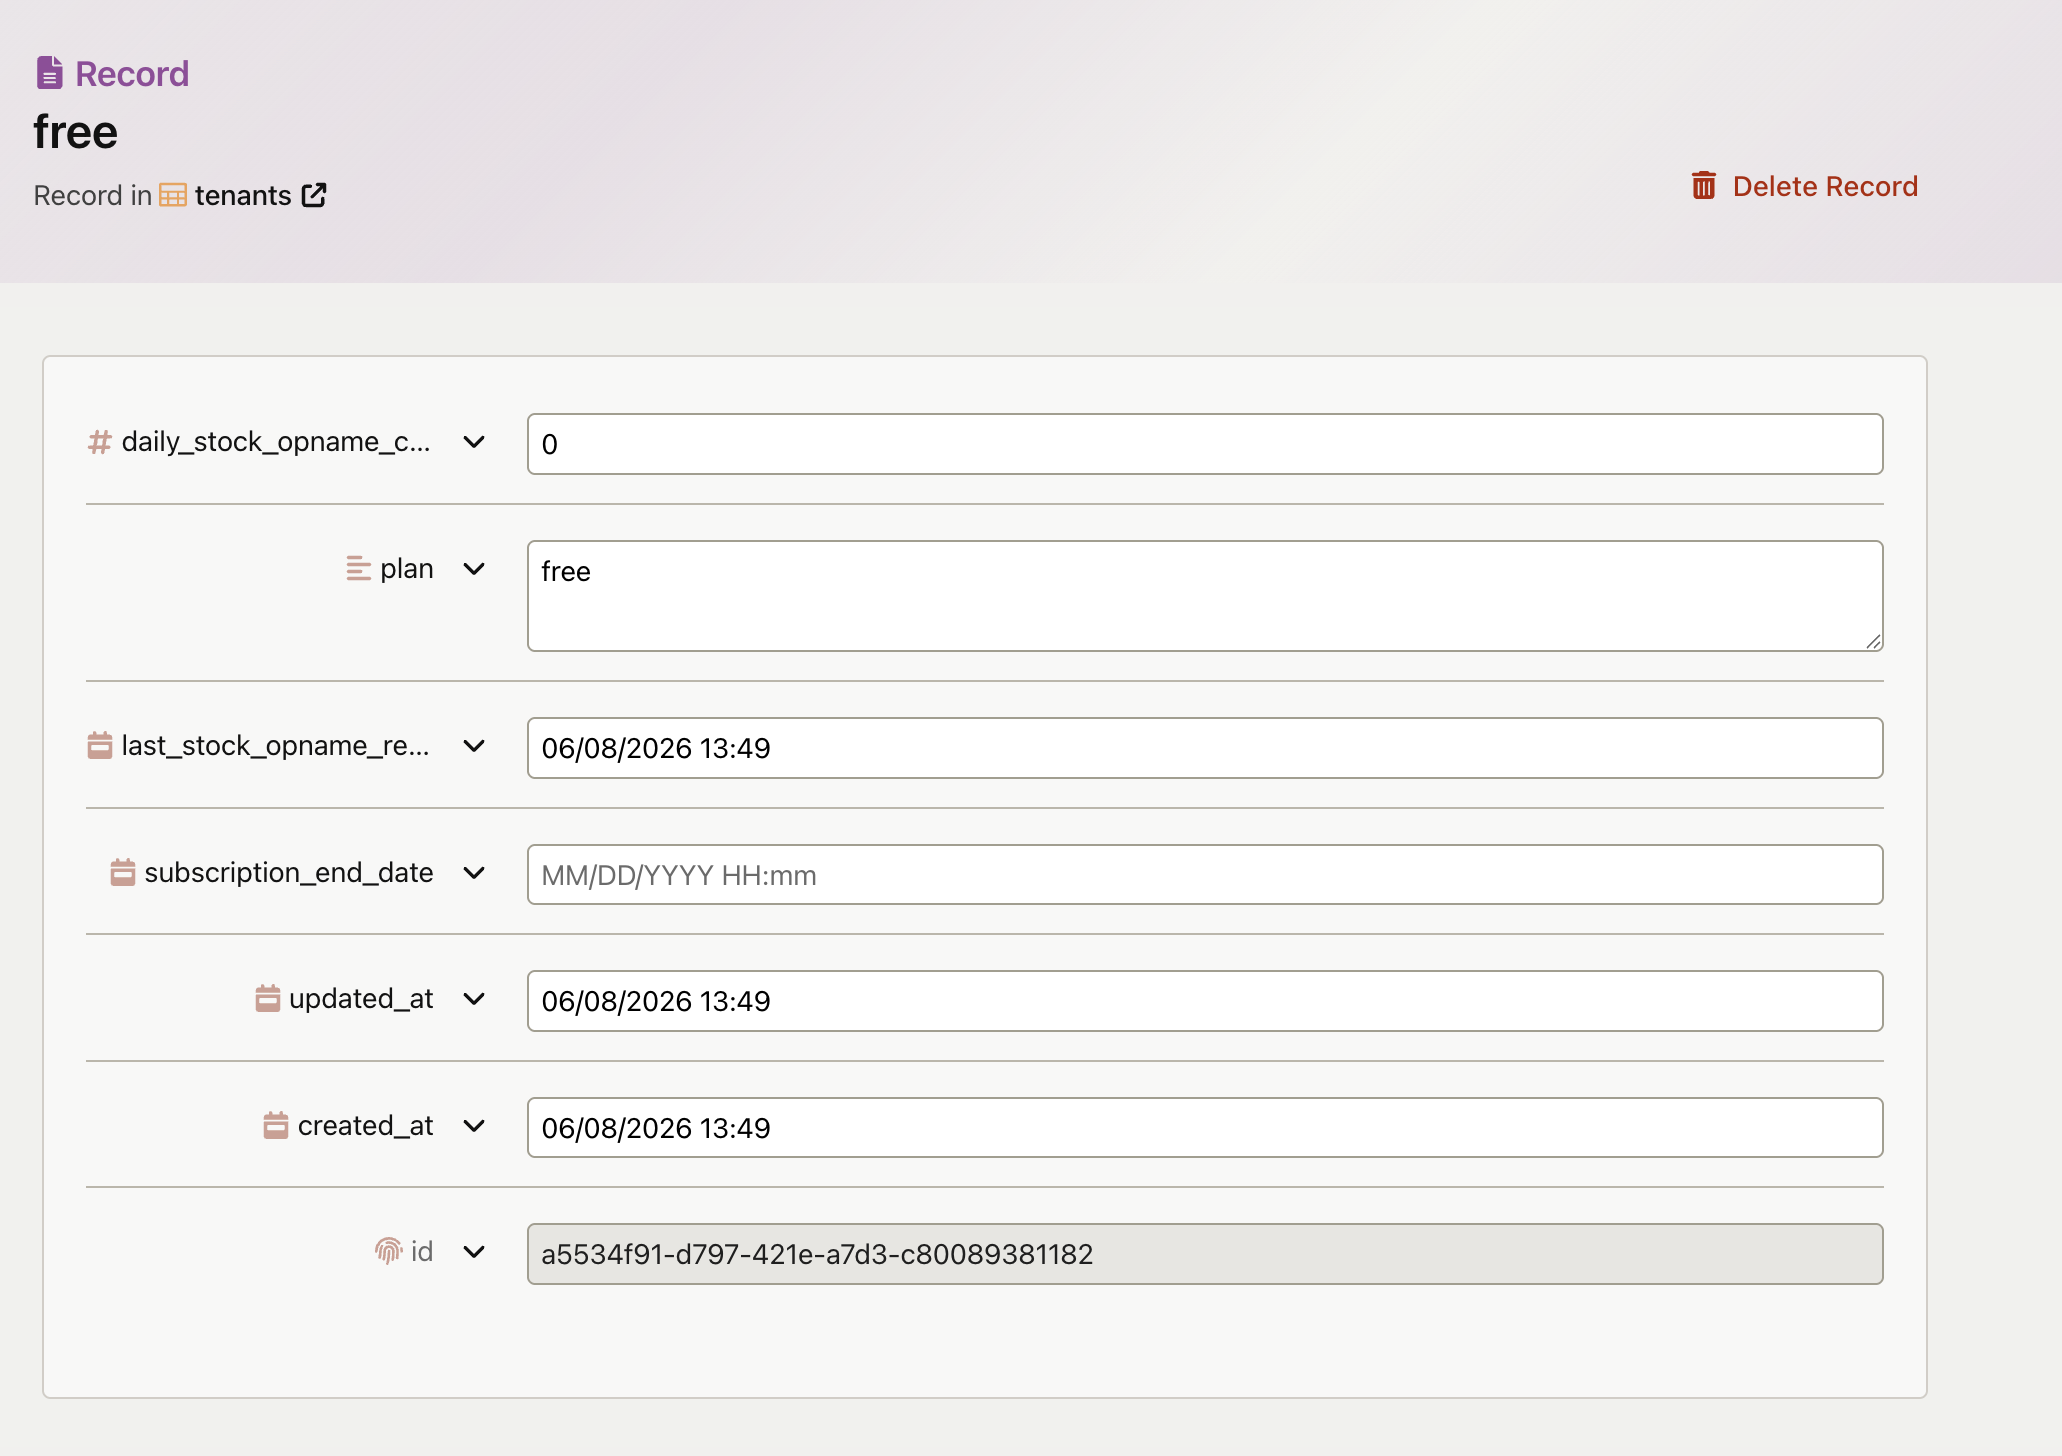
\includegraphics[width=0.9\textwidth]{assets/bab4/test2/table-tenant.png}
  \caption{Data \textit{Tenant} yang Berhasil Dibuat}
  \label{fig:data_tenant_baru}
\end{figure}

Berdasarkan Gambar \ref{fig:data_tenant_baru}, sistem berhasil membuat data \textit{tenant} baru dan menghasilkan identitas \textit{tenant} (\textit{tenant\_id}) yang digunakan sebagai referensi pada proses berikutnya. Identitas tersebut menjadi dasar untuk menghubungkan seluruh data yang dimiliki oleh \textit{tenant}.

Tahap berikutnya adalah pembuatan \textit{role} administrator yang akan digunakan untuk mengelola \textit{tenant} yang baru terdaftar. Hasil pembentukan \textit{role} administrator ditunjukkan pada Gambar \ref{fig:data_role_administrator}.

\begin{figure}[H]
  \centering
  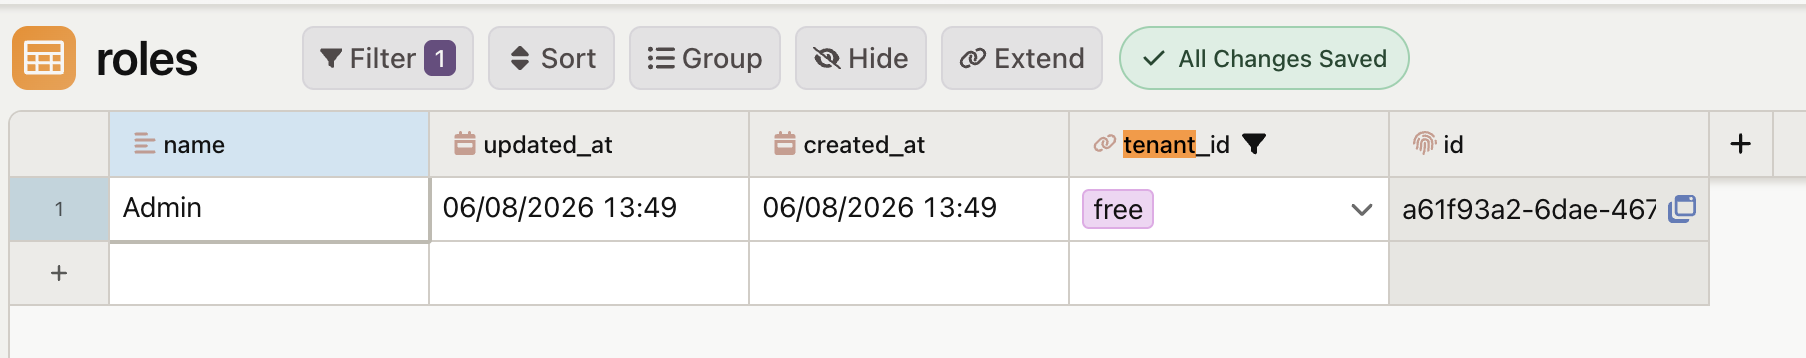
\includegraphics[width=0.9\textwidth]{assets/bab4/test2/table-role.png}
  \caption{Data \textit{Role} Administrator \textit{Tenant}}
  \label{fig:data_role_administrator}
\end{figure}

Hasil pada Gambar \ref{fig:data_role_administrator} menunjukkan bahwa sistem berhasil membuat \textit{role} administrator yang terhubung dengan \textit{tenant} yang baru dibuat. \textit{Role} tersebut digunakan sebagai dasar dalam pengelolaan hak akses pengguna pada \textit{tenant} terkait.

Setelah \textit{role} administrator berhasil dibuat, sistem secara otomatis memberikan hak akses melalui relasi antara \textit{role} dan \textit{permission}. Hasil proses tersebut ditunjukkan pada Gambar \ref{fig:relasi_role_permission}.

\begin{figure}[H]
  \centering
  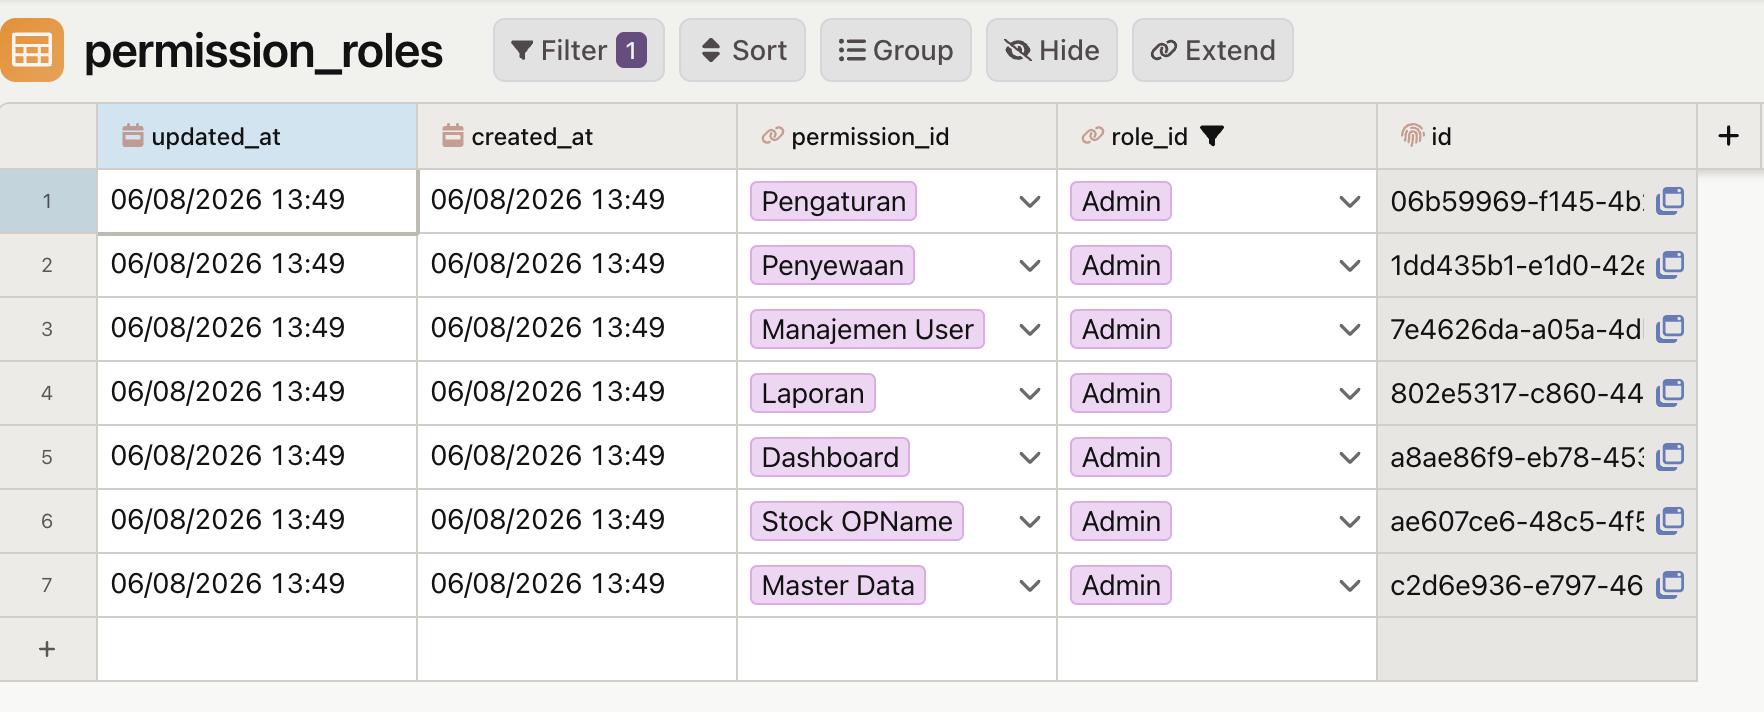
\includegraphics[width=0.9\textwidth]{assets/bab4/test2/table-permission.png}
  \caption{Relasi \textit{Role} Administrator dengan \textit{Permission}}
  \label{fig:relasi_role_permission}
\end{figure}

Berdasarkan Gambar \ref{fig:relasi_role_permission}, \textit{role} administrator berhasil dikaitkan dengan seluruh \textit{permission} yang diperlukan untuk mengakses fitur sistem. Dengan konfigurasi tersebut, administrator \textit{tenant} dapat melakukan pengelolaan data tanpa memerlukan konfigurasi tambahan setelah proses registrasi selesai.

Selanjutnya, sistem membuat akun administrator berdasarkan informasi yang diberikan saat registrasi. Hasil pembentukan akun administrator ditunjukkan pada Gambar \ref{fig:data_akun_administrator}.

\begin{figure}[H]
  \centering
  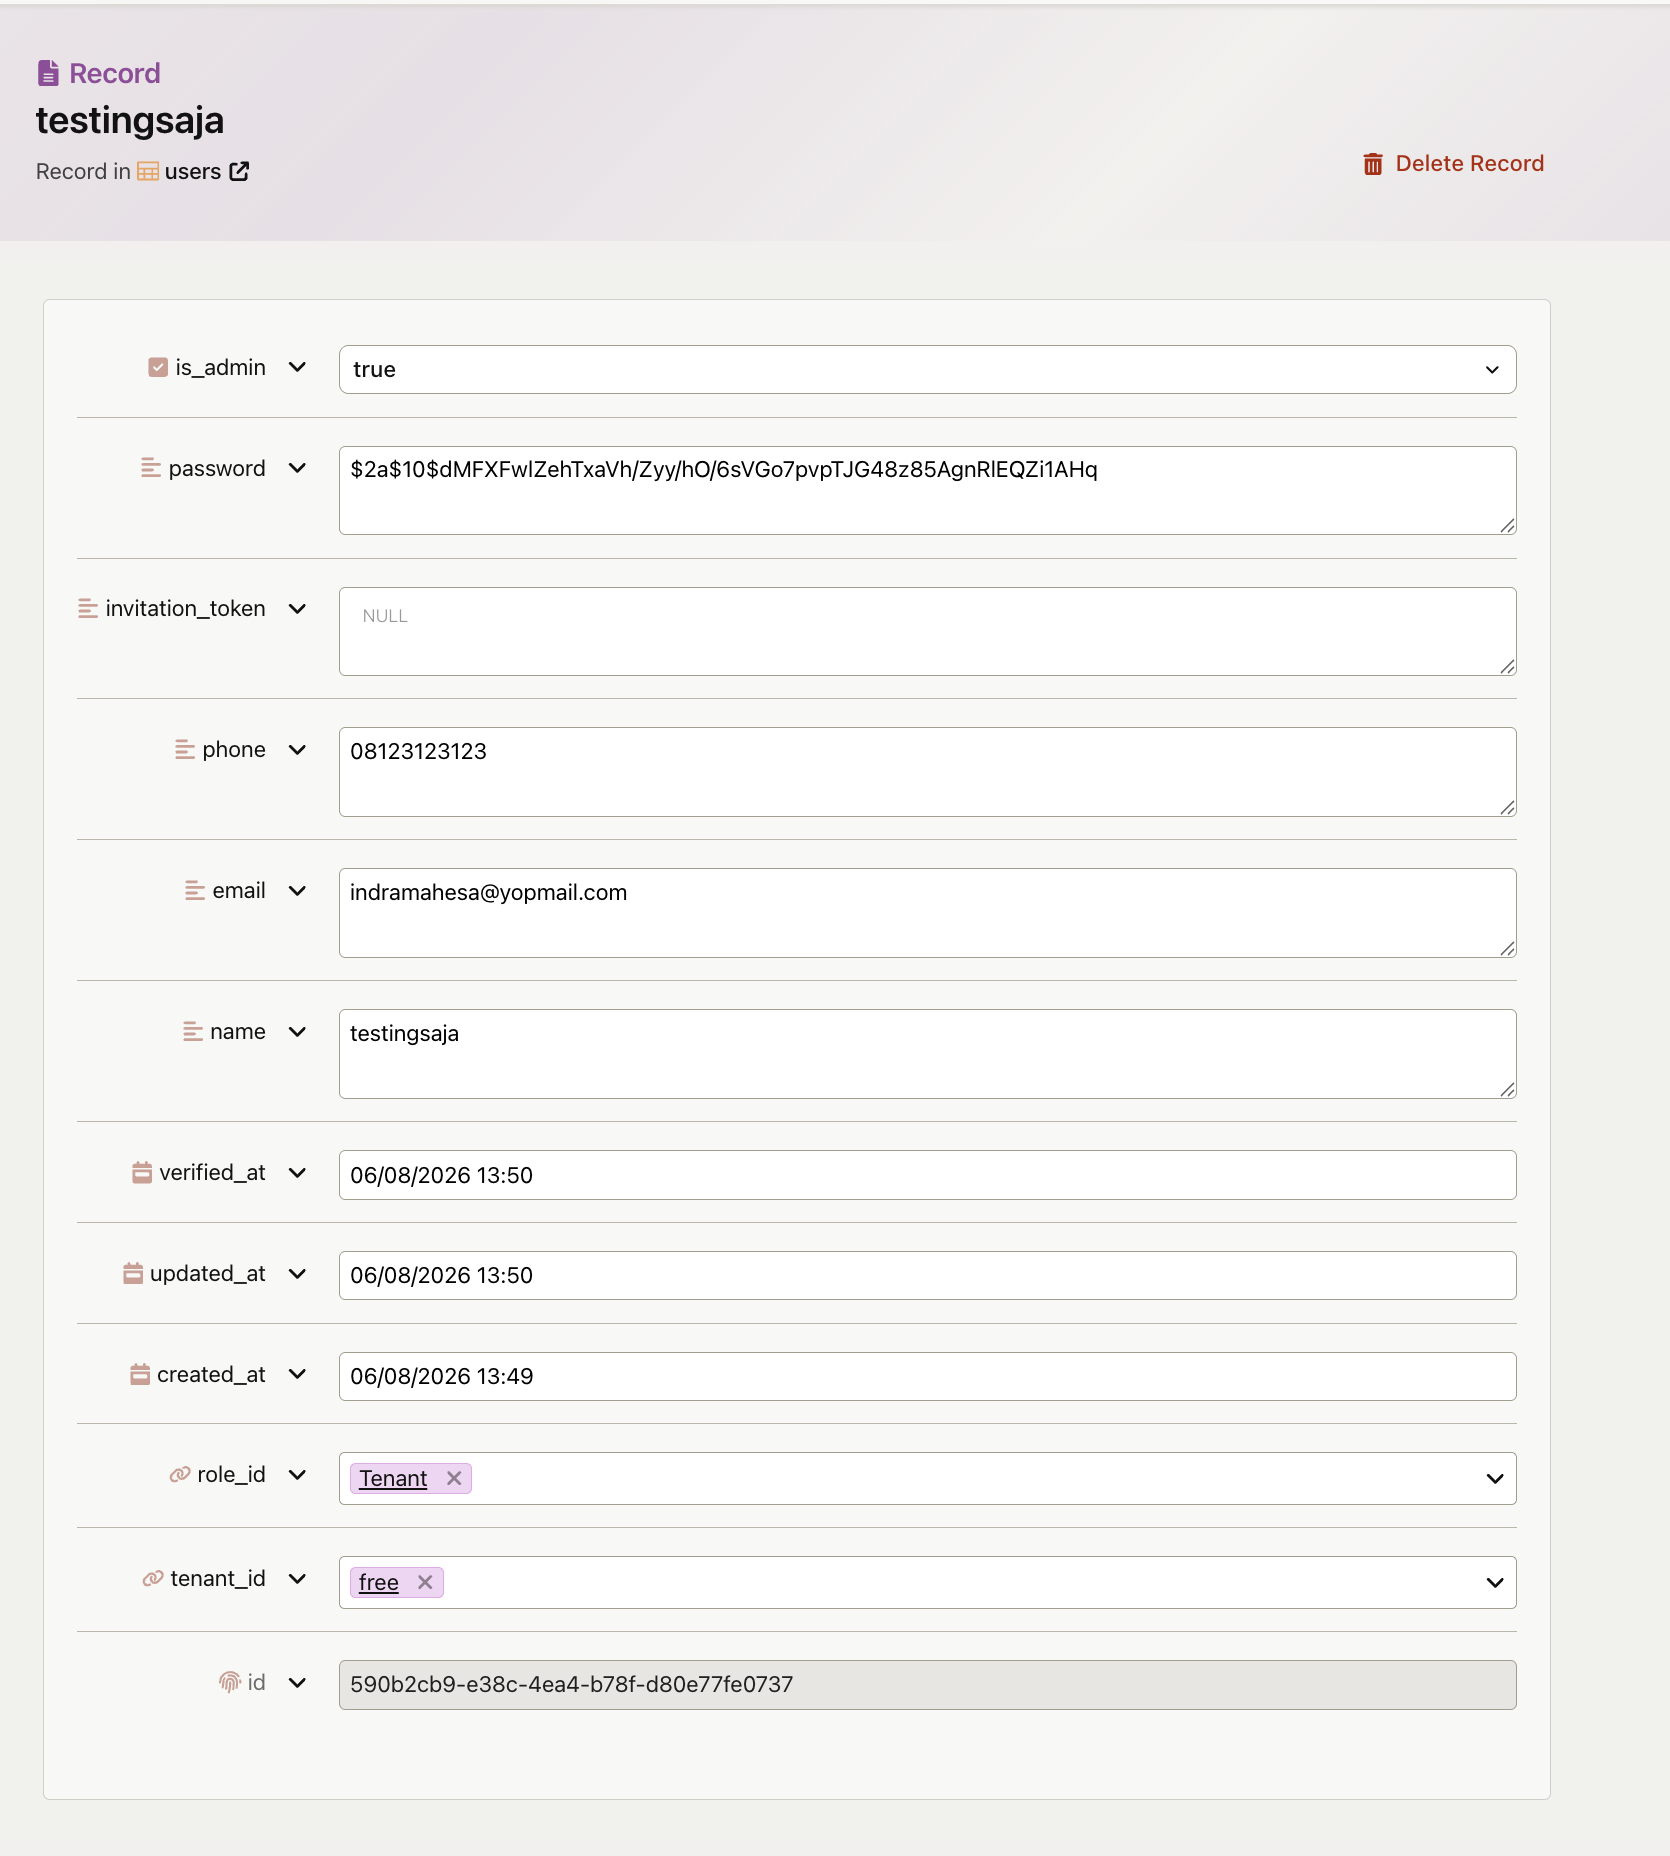
\includegraphics[width=0.9\textwidth]{assets/bab4/test2/table-user.png}
  \caption{Data Akun Administrator \textit{Tenant}}
  \label{fig:data_akun_administrator}
\end{figure}

Berdasarkan Gambar \ref{fig:data_akun_administrator}, akun administrator berhasil dibuat dan dikaitkan dengan \textit{tenant} yang sesuai. Selain itu, akun tersebut juga telah terhubung dengan \textit{role} administrator yang sebelumnya dibuat oleh sistem.

Untuk mempermudah evaluasi hasil pengujian, ringkasan hasil pengujian \textit{tenant provisioning} disajikan pada Tabel \ref{tab:hasil_pengujian_tenant_provisioning}.

\begin{table}[H]
  \centering
  \caption{Hasil Pengujian \textit{Tenant Provisioning}}
  \label{tab:hasil_pengujian_tenant_provisioning}
  \footnotesize
  \begin{tabular}{|l|>{\raggedright\arraybackslash}p{4.5cm}|>{\raggedright\arraybackslash}p{4.5cm}|>{\raggedright\arraybackslash}p{2.5cm}|}
    \hline
    \rowcolor[HTML]{EFEFEF}
    \textbf{No} & \textbf{Skenario Pengujian} & \textbf{Hasil yang Diharapkan} & \textbf{Hasil Pengujian} \\
    \hline
    1 & Registrasi \textit{tenant} baru & Data \textit{tenant} berhasil dibuat & Berhasil \\
    \hline
    2 & Pembuatan \textit{role} administrator & \textit{Role} administrator berhasil dibuat & Berhasil \\
    \hline
    3 & Pemberian \textit{permission} & \textit{Permission} berhasil dikaitkan dengan \textit{role} administrator & Berhasil \\
    \hline
    4 & Pembuatan akun administrator & Akun administrator berhasil dibuat & Berhasil \\
    \hline
    5 & Relasi pengguna dan \textit{role} & Pengguna berhasil dikaitkan dengan \textit{role} administrator & Berhasil \\
    \hline
    6 & Login menggunakan akun administrator & Pengguna berhasil masuk ke sistem & Berhasil \\
    \hline
  \end{tabular}
\end{table}

Berdasarkan hasil pengujian pada Tabel \ref{tab:hasil_pengujian_tenant_provisioning}, seluruh tahapan \textit{tenant provisioning} berhasil dijalankan sesuai dengan hasil yang diharapkan. Sistem mampu membuat \textit{tenant} baru beserta \textit{role} administrator, \textit{permission}, dan akun administrator secara otomatis tanpa memerlukan konfigurasi manual tambahan.

Hasil tersebut menunjukkan bahwa mekanisme \textit{tenant provisioning} yang diterapkan pada penelitian ini mampu mendukung proses \textit{onboarding} \textit{tenant} secara cepat dan konsisten.

\subsection{Hasil Pengujian Shared Database dan Shared Schema}

Pengujian \textit{shared database} dan \textit{shared schema} dilakukan untuk memverifikasi bahwa beberapa \textit{tenant} dapat menggunakan basis data dan struktur tabel yang sama tanpa menyebabkan pencampuran data antar \textit{tenant}. Pengujian ini penting karena pendekatan yang digunakan pada penelitian ini menempatkan seluruh \textit{tenant} pada satu basis data dan satu struktur tabel yang sama. Oleh karena itu, diperlukan verifikasi untuk memastikan bahwa setiap data tetap dapat diidentifikasi berdasarkan \textit{tenant} yang memilikinya.

Pengujian dilakukan dengan menggunakan beberapa \textit{tenant} yang telah terdaftar pada sistem. Setiap \textit{tenant} melakukan aktivitas pengelolaan data sehingga menghasilkan data operasional yang tersimpan pada basis data. Selanjutnya dilakukan pemeriksaan langsung pada tabel-tabel yang digunakan oleh sistem untuk memastikan bahwa data dari beberapa \textit{tenant} dapat disimpan secara bersamaan.

\begin{figure}[H]
  \centering
  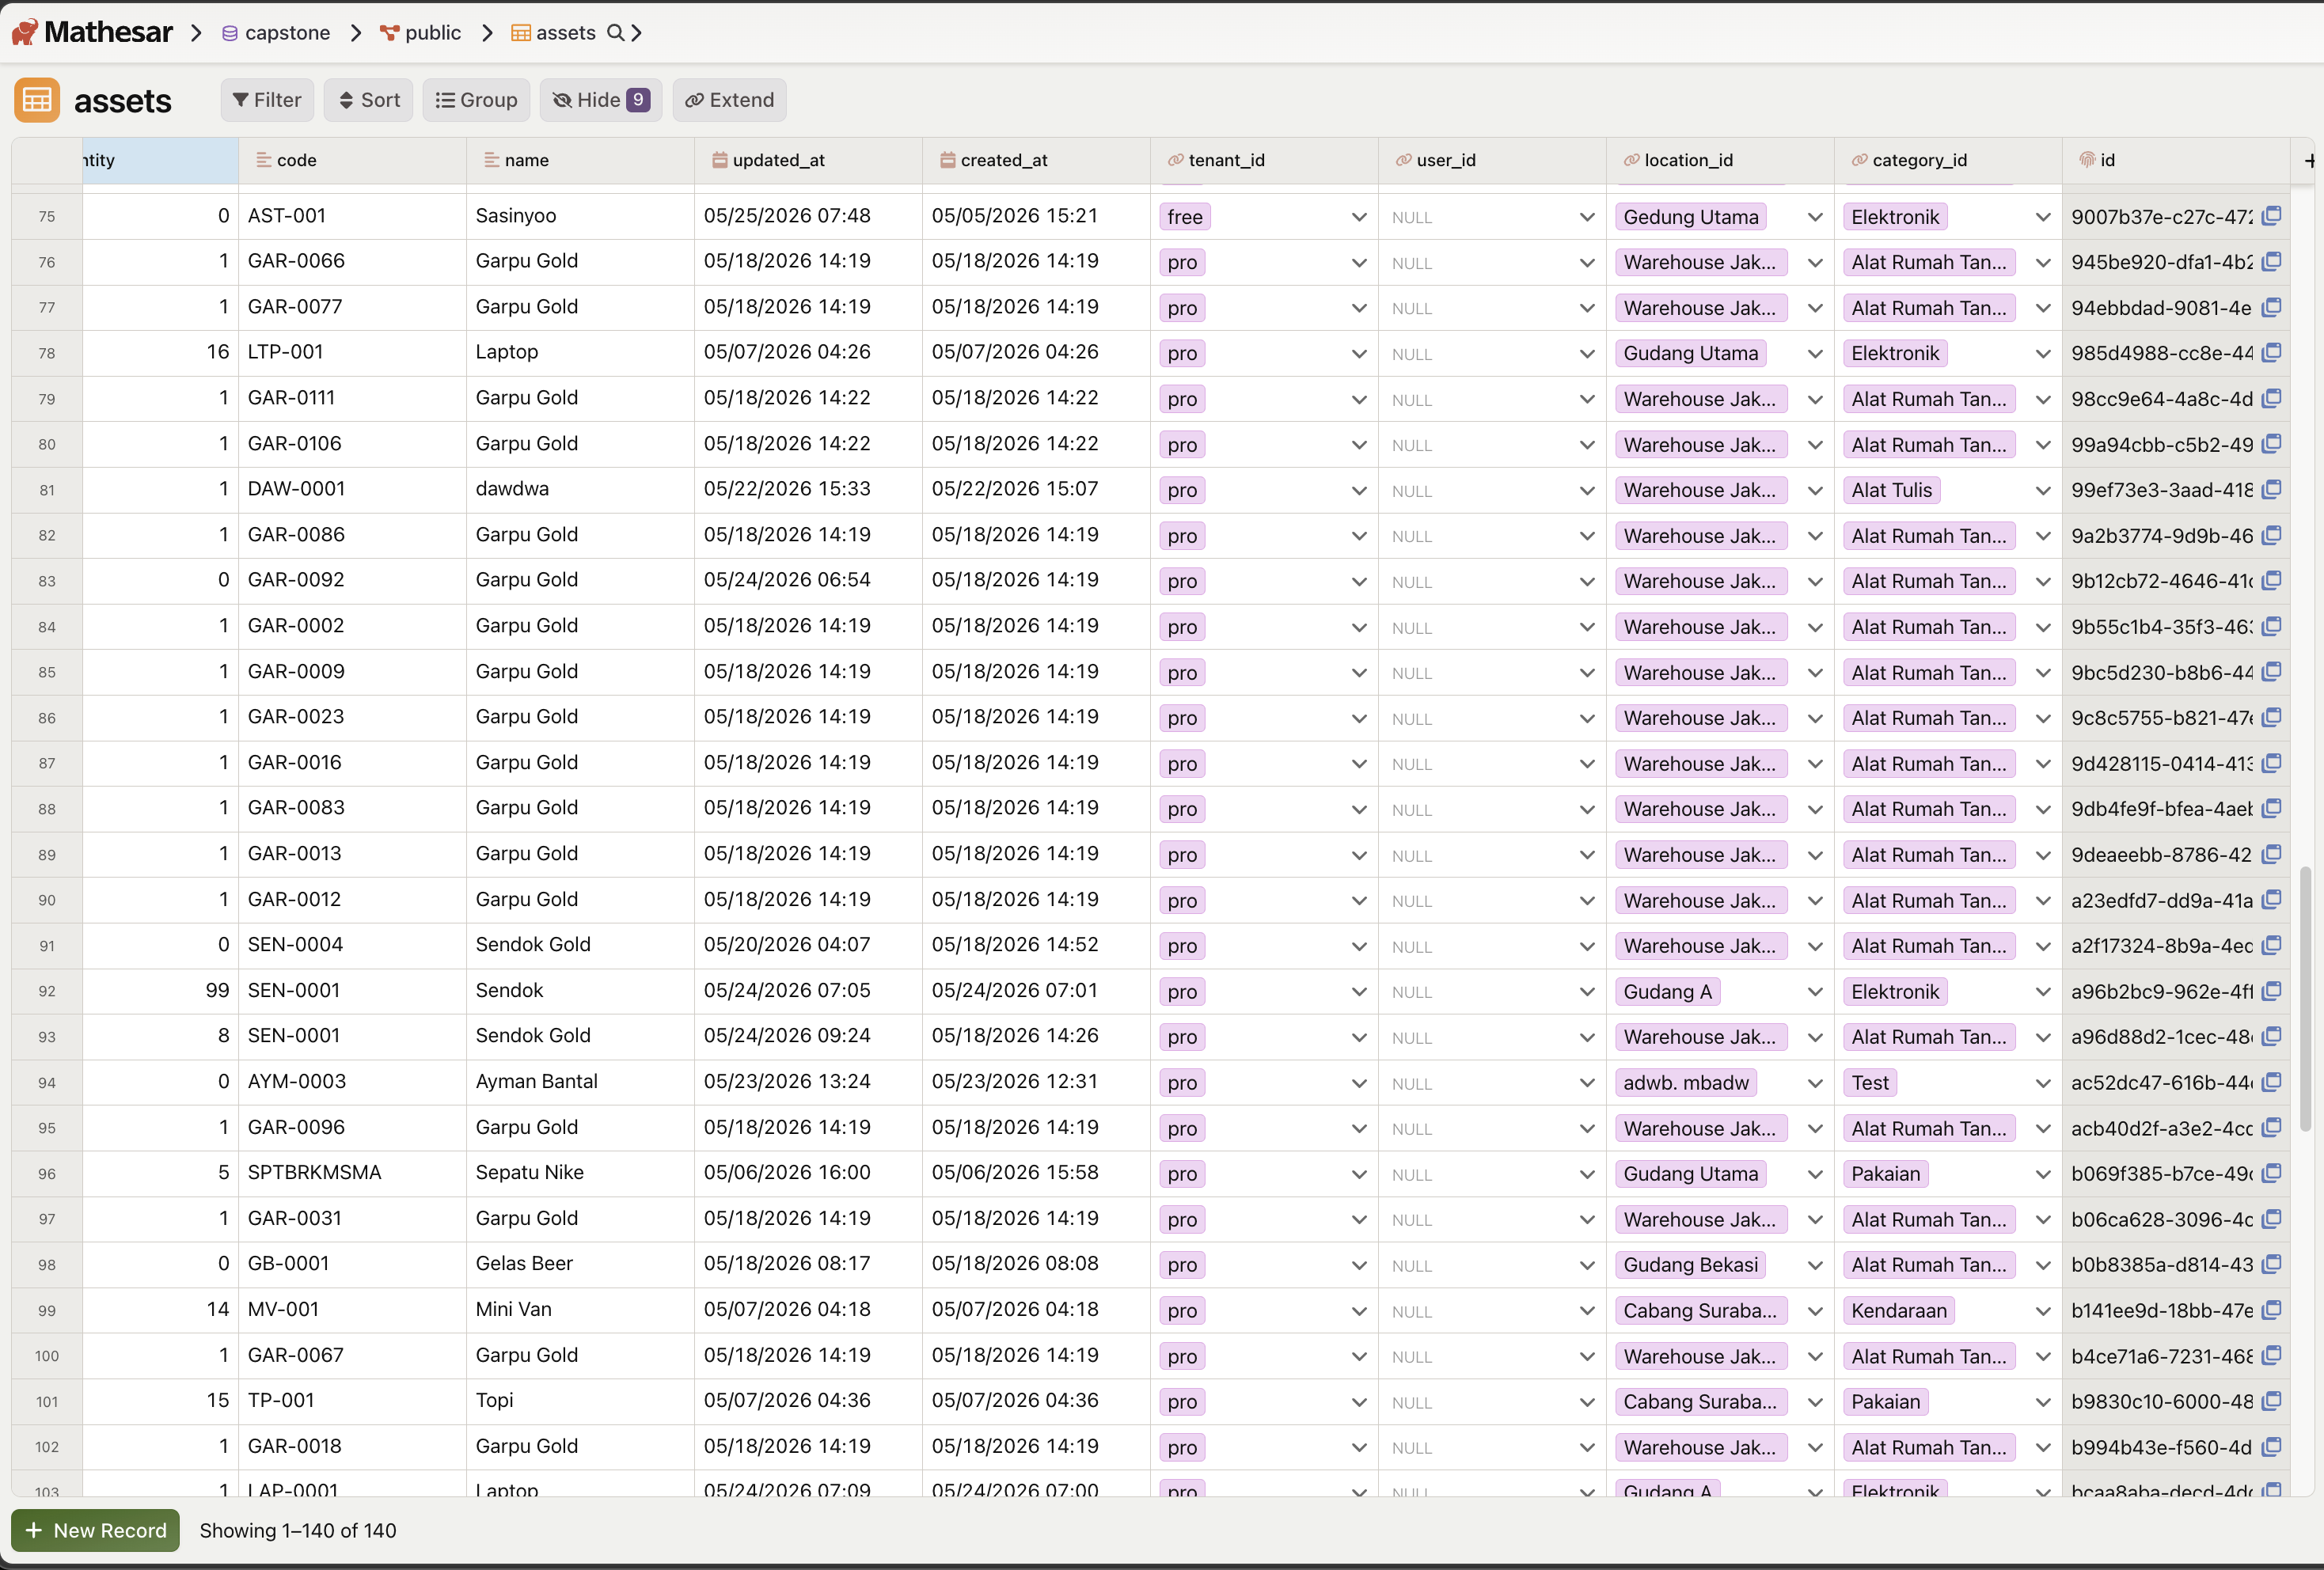
\includegraphics[width=0.9\textwidth]{assets/bab4/test3/table-asset.png}
  \caption{Data Multi \textit{Tenant} pada Tabel \textit{Assets}}
  \label{fig:data_multi_tenant_assets}
\end{figure}

Berdasarkan Gambar \ref{fig:data_multi_tenant_assets}, data aset dari beberapa \textit{tenant} tersimpan pada tabel \textit{assets} yang sama. Meskipun berada dalam satu tabel, setiap data memiliki atribut \textit{tenant\_id} yang berbeda. Atribut tersebut digunakan sebagai identitas \textit{tenant} sehingga sistem dapat membedakan kepemilikan data pada masing-masing \textit{tenant}.

Selain data aset, pengujian juga dilakukan terhadap data pengguna yang tersimpan pada sistem. Hasil pemeriksaan ditunjukkan pada Gambar \ref{fig:data_multi_tenant_users}.

\begin{figure}[H]
  \centering
  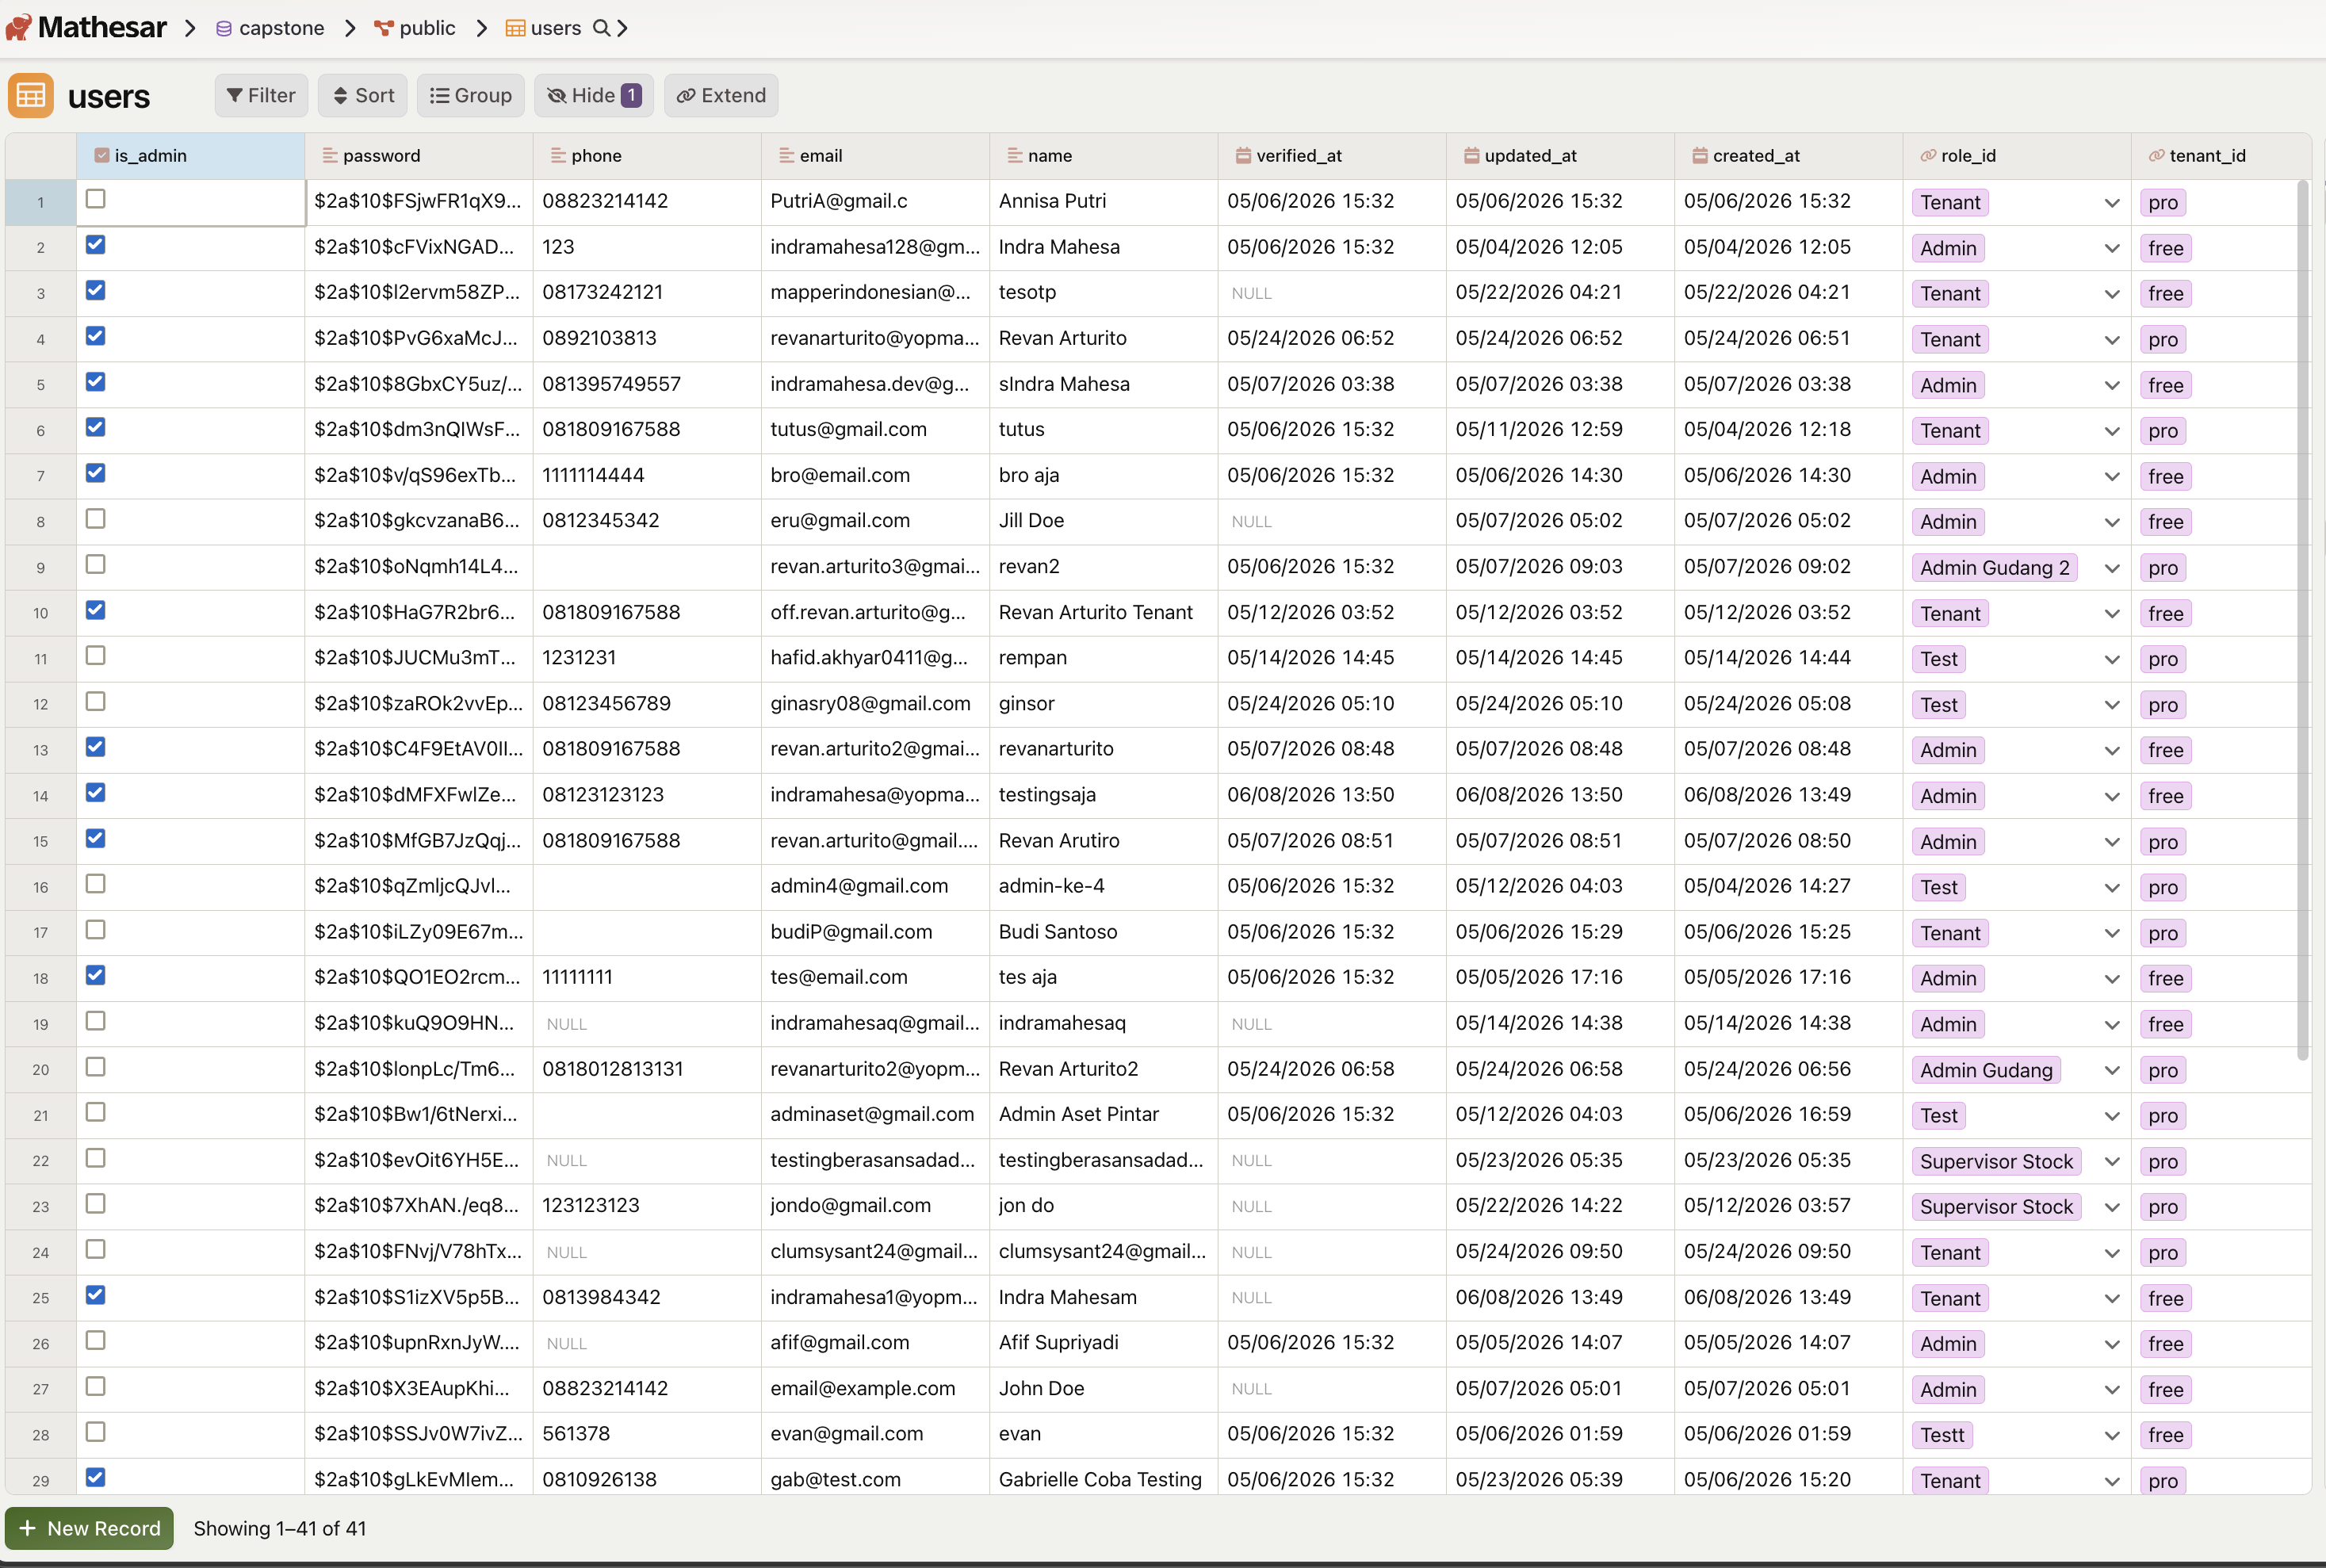
\includegraphics[width=0.9\textwidth]{assets/bab4/test3/table-user.png}
  \caption{Data Multi \textit{Tenant} pada Tabel \textit{Users}}
  \label{fig:data_multi_tenant_users}
\end{figure}

Berdasarkan Gambar \ref{fig:data_multi_tenant_users}, data pengguna dari beberapa \textit{tenant} juga tersimpan pada tabel \textit{users} yang sama. Setiap pengguna tetap memiliki keterkaitan dengan \textit{tenant} yang sesuai melalui atribut \textit{tenant\_id}. Hal tersebut menunjukkan bahwa pendekatan \textit{shared database} dan \textit{shared schema} diterapkan secara konsisten pada tabel yang digunakan oleh sistem.

Untuk memastikan bahwa \textit{tenant} menggunakan struktur tabel yang sama, dilakukan pemeriksaan terhadap skema tabel yang digunakan untuk menyimpan data operasional.

\begin{figure}[H]
  \centering
  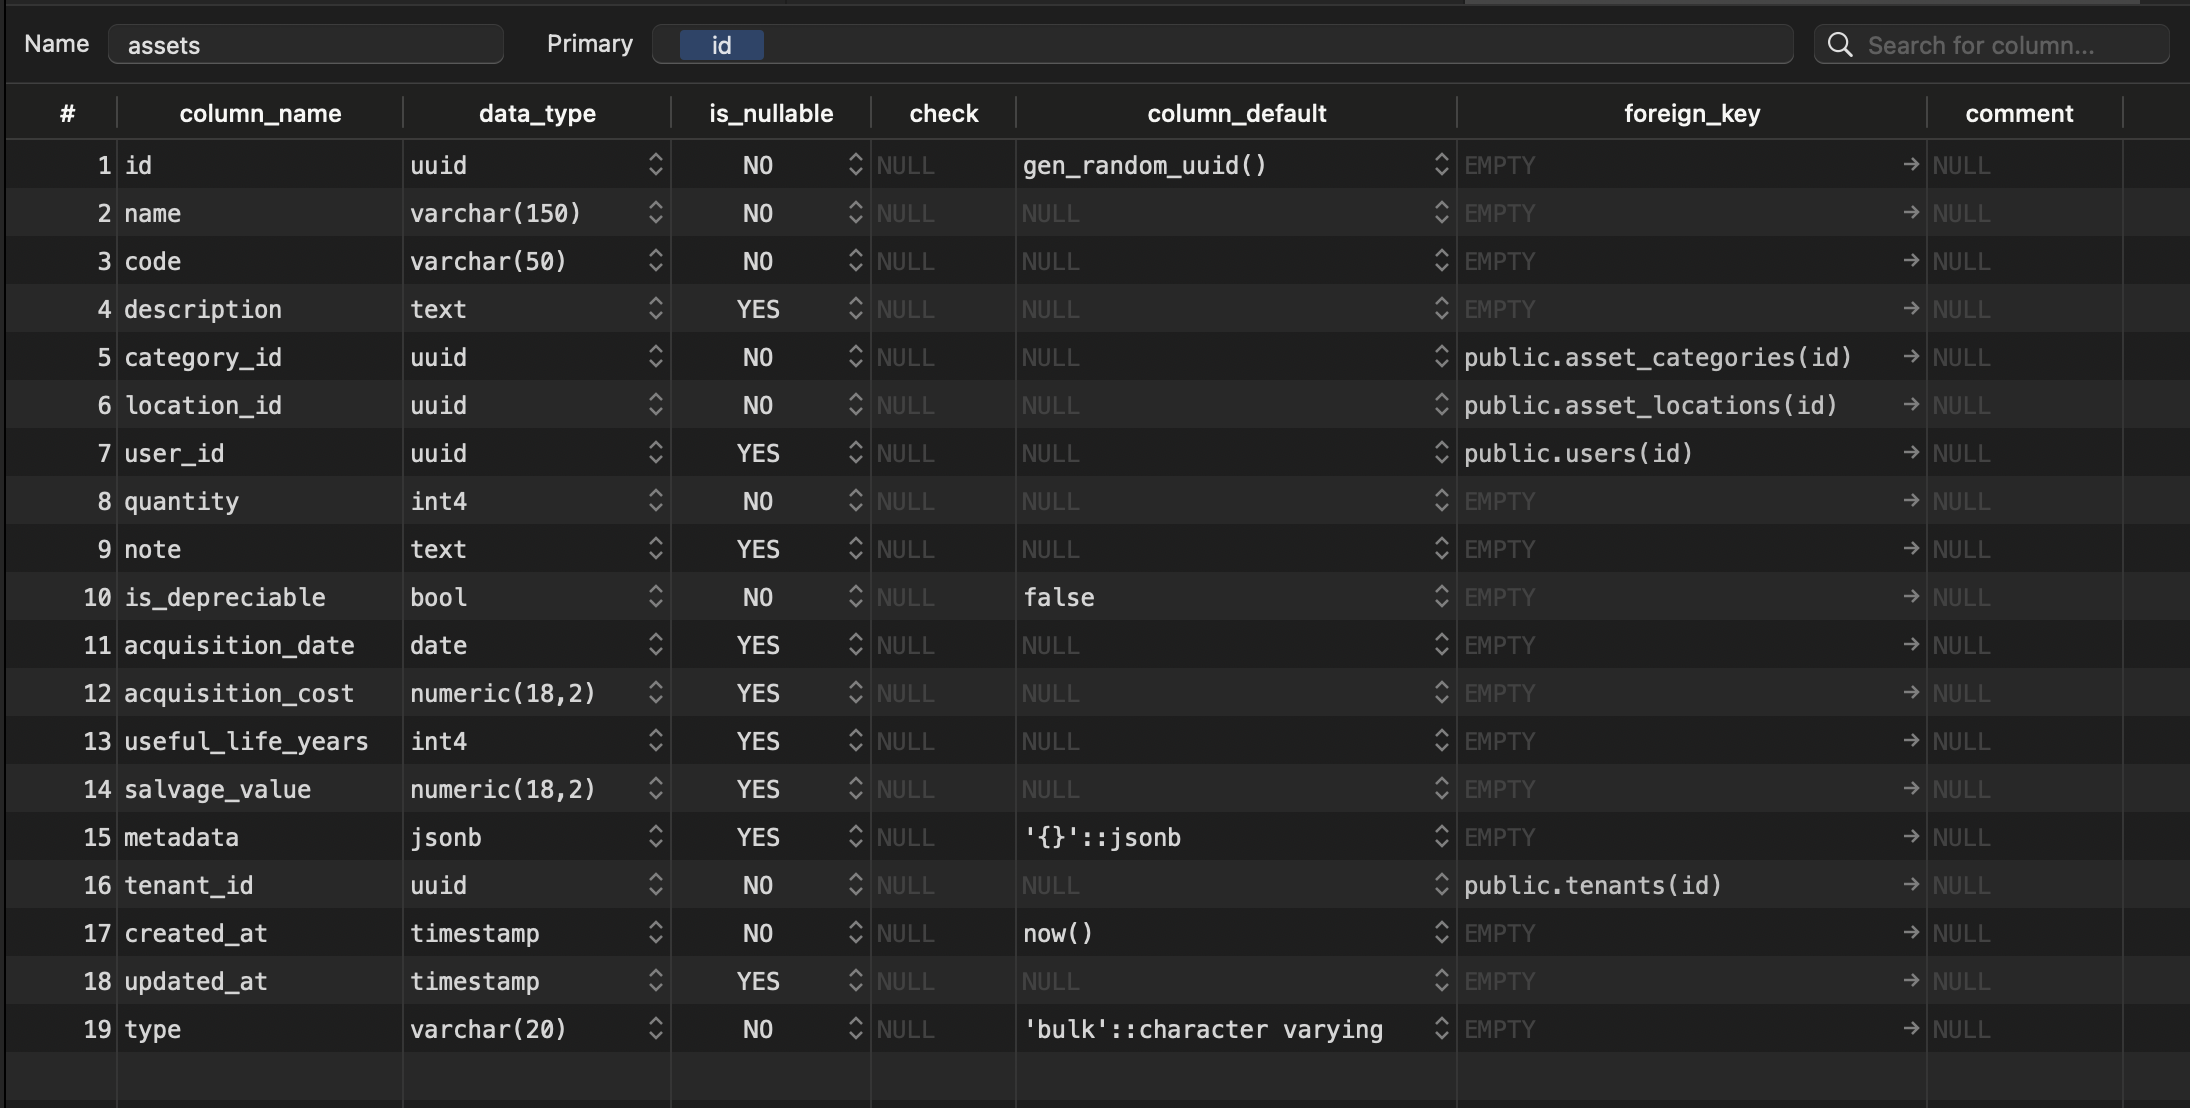
\includegraphics[width=0.9\textwidth]{assets/bab4/test3/structure-asset.png}
  \caption{Struktur Tabel \textit{Assets} pada Basis Data}
  \label{fig:struktur_tabel_assets}
\end{figure}

Gambar \ref{fig:struktur_tabel_assets} menunjukkan bahwa seluruh \textit{tenant} menggunakan struktur tabel yang sama untuk menyimpan data aset. Tidak terdapat tabel khusus untuk masing-masing \textit{tenant} sehingga seluruh data dikelola menggunakan satu skema basis data yang sama. Pendekatan ini memungkinkan pengelolaan basis data menjadi lebih sederhana dibandingkan penggunaan basis data atau tabel terpisah untuk setiap \textit{tenant}.

Hasil pengujian juga menunjukkan bahwa proses penyimpanan data dari \textit{tenant} yang berbeda dapat dilakukan tanpa menimbulkan konflik pada struktur basis data. Identifikasi \textit{tenant} dilakukan menggunakan atribut \textit{tenant\_id} yang disimpan pada setiap data operasional.

Ringkasan hasil pengujian \textit{shared database} dan \textit{shared schema} ditunjukkan pada Tabel \ref{tab:hasil_pengujian_shared_database}.

\begin{table}[H]
  \centering
  \caption{Hasil Pengujian \textit{Shared Database} dan \textit{Shared Schema}}
  \label{tab:hasil_pengujian_shared_database}
  \footnotesize
  \begin{tabular}{|l|>{\raggedright\arraybackslash}p{3.2cm}|>{\raggedright\arraybackslash}p{3.5cm}|>{\raggedright\arraybackslash}p{3.5cm}|>{\raggedright\arraybackslash}p{1.8cm}|}
    \hline
    \rowcolor[HTML]{EFEFEF}
    \textbf{No} & \textbf{Skenario Pengujian} & \textbf{Hasil yang Diharapkan} & \textbf{Hasil Aktual} & \textbf{Status} \\
    \hline
    1 & Tenant A menambahkan data aset & Data berhasil tersimpan pada tabel \textit{assets} & Data berhasil tersimpan pada tabel \textit{assets} & Berhasil \\
    \hline
    2 & Tenant B menambahkan data aset & Data berhasil tersimpan pada tabel \textit{assets} & Data berhasil tersimpan pada tabel \textit{assets} & Berhasil \\
    \hline
    3 & Pemeriksaan tabel \textit{assets} & Data beberapa \textit{tenant} berada pada tabel yang sama & Data beberapa \textit{tenant} berada pada tabel yang sama & Berhasil \\
    \hline
    4 & Pemeriksaan tabel \textit{users} & Data beberapa \textit{tenant} berada pada tabel yang sama & Data beberapa \textit{tenant} berada pada tabel yang sama & Berhasil \\
    \hline
    5 & Pemeriksaan atribut \textit{tenant\_id} & Setiap data memiliki identitas \textit{tenant} yang sesuai & Setiap data memiliki identitas \textit{tenant} yang sesuai & Berhasil \\
    \hline
    6 & Pemeriksaan struktur tabel & Seluruh \textit{tenant} menggunakan struktur tabel yang sama & Seluruh \textit{tenant} menggunakan struktur tabel yang sama & Berhasil \\
    \hline
  \end{tabular}
\end{table}

Berdasarkan hasil pengujian pada Tabel \ref{tab:hasil_pengujian_shared_database}, seluruh skenario pengujian berhasil dijalankan sesuai dengan hasil yang diharapkan. Data dari beberapa \textit{tenant} dapat disimpan pada tabel yang sama tanpa menyebabkan pencampuran data. Selain itu, setiap data tetap memiliki identitas \textit{tenant} yang dapat digunakan untuk membedakan kepemilikan data pada masing-masing \textit{tenant}.

Hasil tersebut menunjukkan bahwa implementasi \textit{shared database} dan \textit{shared schema} pada penelitian ini berhasil diterapkan sesuai dengan rancangan sistem. Pendekatan tersebut memungkinkan beberapa \textit{tenant} menggunakan basis data dan struktur tabel yang sama, namun tetap mendukung mekanisme pemisahan data melalui penggunaan atribut \textit{tenant\_id}.

\section{Analisis}

\subsection{Analisis Tenant Isolation}

Berdasarkan hasil pengujian yang telah dilakukan pada Subbab 4.3.1, mekanisme \textit{tenant isolation} berhasil diterapkan pada sistem sesuai dengan rancangan yang telah dijelaskan pada Bab 3. Hasil pengujian menunjukkan bahwa pengguna hanya dapat mengakses data yang berada dalam ruang lingkup \textit{tenant} yang sesuai dengan identitas \textit{tenant} yang dimiliki pengguna tersebut.

Pada pengujian menggunakan akun \textbf{gab@test.com} dan \textbf{indramahesa128@gmail.com}, sistem menampilkan data aset yang berbeda untuk masing-masing pengguna meskipun data tersebut tersimpan pada basis data dan tabel yang sama. Hasil tersebut menunjukkan bahwa sistem berhasil melakukan pemfilteran data berdasarkan identitas \textit{tenant} sebelum data dikembalikan kepada pengguna.

Selain melalui antarmuka aplikasi, hasil pengujian pada layanan API juga menunjukkan bahwa data yang dikembalikan sistem hanya berasal dari \textit{tenant} yang sedang aktif. Informasi \textit{tenant} yang tersimpan pada token autentikasi digunakan sebagai dasar untuk membatasi ruang lingkup akses data. Dengan mekanisme tersebut, pengguna tidak dapat memperoleh data milik \textit{tenant} lain meskipun menggunakan \textit{endpoint} API yang sama.

Berdasarkan indikator keberhasilan yang telah ditetapkan pada Bab 3, seluruh skenario pengujian \textit{tenant isolation} berhasil memenuhi kriteria yang diharapkan. Pengguna tidak dapat melihat, mengubah, maupun menghapus data yang dimiliki \textit{tenant} lain. Hasil tersebut menunjukkan bahwa mekanisme \textit{tenant isolation} yang diterapkan mampu menjaga pemisahan data antar \textit{tenant} secara konsisten pada lapisan aplikasi, layanan API, dan basis data.

\subsection{Analisis Tenant Provisioning}

Berdasarkan hasil pengujian pada Subbab 4.3.2, proses \textit{tenant provisioning} berhasil dijalankan sesuai dengan rancangan sistem yang telah dibuat. Seluruh tahapan yang dirancang, mulai dari registrasi \textit{tenant}, verifikasi email menggunakan kode OTP, hingga pembentukan data \textit{tenant} dan akun administrator, berhasil dilakukan secara otomatis oleh sistem.

Hasil pengujian menunjukkan bahwa setelah pengguna menyelesaikan proses registrasi dan verifikasi email, sistem secara otomatis membentuk data \textit{tenant}, \textit{role} administrator, relasi \textit{permission}, dan akun administrator tanpa memerlukan konfigurasi manual tambahan. Pendekatan tersebut memungkinkan \textit{tenant} yang baru terdaftar dapat langsung menggunakan sistem setelah proses registrasi selesai dilakukan.

Selain meningkatkan efisiensi proses \textit{onboarding} \textit{tenant}, mekanisme \textit{tenant provisioning} juga membantu menjaga konsistensi konfigurasi pada setiap \textit{tenant} yang terdaftar. Seluruh \textit{tenant} memperoleh struktur \textit{role} dan hak akses awal yang seragam sehingga risiko kesalahan konfigurasi dapat diminimalkan.

Berdasarkan indikator keberhasilan yang telah ditetapkan pada Bab 3, seluruh kasus uji pada proses \textit{tenant provisioning} berhasil memenuhi hasil yang diharapkan. Dengan demikian, mekanisme yang diterapkan pada penelitian ini mampu mendukung proses pendaftaran \textit{tenant} baru secara otomatis dan mempersingkat proses aktivasi \textit{tenant} pada sistem \textit{multitenant}.

\subsection{Analisis Shared Database dan Shared Schema}

Berdasarkan hasil pengujian pada Subbab 4.3.3, implementasi \textit{shared database} dan \textit{shared schema} berhasil diterapkan sesuai dengan rancangan yang diusulkan. Hasil pemeriksaan basis data menunjukkan bahwa data dari beberapa \textit{tenant} dapat disimpan pada basis data dan struktur tabel yang sama tanpa menyebabkan pencampuran data antar \textit{tenant}.

Penggunaan atribut \textit{tenant\_id} pada setiap data operasional memungkinkan sistem mengidentifikasi kepemilikan data dari masing-masing \textit{tenant}. Meskipun data aset dan pengguna berada pada tabel yang sama, setiap data tetap dapat dibedakan berdasarkan identitas \textit{tenant} yang dimiliki. Hasil tersebut menunjukkan bahwa pendekatan \textit{shared database} dan \textit{shared schema} dapat digunakan tanpa mengurangi kemampuan sistem dalam menjaga pemisahan data.

Penerapan pendekatan ini juga memberikan keuntungan dalam pengelolaan basis data karena seluruh \textit{tenant} menggunakan struktur tabel yang sama. Dengan demikian, proses pengembangan dan pemeliharaan basis data dapat dilakukan secara lebih sederhana dibandingkan pendekatan yang menggunakan basis data atau tabel terpisah untuk setiap \textit{tenant}.

Berdasarkan indikator keberhasilan yang telah ditetapkan pada Bab 3, seluruh skenario pengujian berhasil memenuhi kriteria yang diharapkan. Data dari beberapa \textit{tenant} berhasil disimpan pada tabel yang sama dan tetap dapat dipisahkan melalui atribut \textit{tenant\_id}. Hasil tersebut menunjukkan bahwa implementasi \textit{shared database} dan \textit{shared schema} yang digunakan pada penelitian ini berhasil mendukung kebutuhan arsitektur \textit{multitenant} yang diterapkan pada sistem.

\chapter{Penutup}

\section{Kesimpulan}

Berdasarkan hasil penelitian dan pembahasan yang telah dilakukan, dapat disimpulkan bahwa:
\begin{enumerate}
  \item Kesimpulan pertama berdasarkan rumusan masalah pertama.
  \item Kesimpulan kedua berdasarkan rumusan masalah kedua.
\end{enumerate}

\section{Saran}

Berdasarkan hasil penelitian, saran yang dapat diberikan adalah:
\begin{enumerate}
  \item Saran untuk penelitian selanjutnya.
  \item Saran untuk pengembangan lebih lanjut.
\end{enumerate}


%------------------------------------------------------------------------------
% DAFTAR PUSTAKA
%------------------------------------------------------------------------------
\bibliographystyle{apalike}
\nocite{*} % Tampilkan semua referensi meski belum dikutip; hapus saat selesai
\bibliography{references/daftar_pustaka}

%------------------------------------------------------------------------------
% LAMPIRAN
%------------------------------------------------------------------------------
\appendix
\chapter*{LAMPIRAN}
\addcontentsline{toc}{chapter}{LAMPIRAN}

% TODO: Tambahkan lampiran jika diperlukan


\end{document}
